\documentclass[10pt]{extarticle}

\usepackage[english]{babel}
\usepackage{graphicx}
\usepackage{framed}
\usepackage[normalem]{ulem}
\usepackage{indentfirst}
\usepackage{amsmath,amsthm,amssymb,amsfonts}
\usepackage[italicdiff]{physics}
\usepackage[T1]{fontenc}
%\usepackage{pifont} %For unusual symbols
%\usepackage{mathdots} %For unusual combinations of dots
\usepackage{wrapfig}
\usepackage{lmodern,mathrsfs}
\usepackage[inline,shortlabels]{enumitem}
\setlist{topsep=2pt,itemsep=2pt,parsep=0pt,partopsep=0pt}
\usepackage[dvipsnames]{xcolor}
\usepackage[utf8]{inputenc}
\usepackage[a4paper, top=0.5in,bottom=0.2in, left=0.5in, right=0.5in, footskip=0.3in, includefoot]{geometry}
\usepackage[most]{tcolorbox}
\usepackage{tikz,tikz-3dplot,tikz-cd,tkz-tab,tkz-euclide,pgf,pgfplots}
\pgfplotsset{compat=newest}
\usepackage{multicol}
\usepackage[bottom,multiple]{footmisc} %ensures footnotes are at the bottom of the page, and separates footnotes by a comma if they are adjacent
\usepackage[backend=bibtex,style=numeric]{biblatex}
\renewcommand*{\finalnamedelim}{\addcomma\addspace} %forces authors' names to be separated by comma, instead of "and"
\addbibresource{bibliography}
\usepackage{hyperref}
\usepackage[nameinlink]{cleveref} %nameinlink ensures that the entire element is clickable in the pdf, not just the number

\newcommand{\remind}[1]{\textcolor{red}{\textbf{#1}}} %To remind me of unfinished work to fix later
\newcommand{\hide}[1]{} %To hide large blocks of code without using % symbols

\newcommand{\ep}{\varepsilon}
\newcommand{\vp}{\varphi}
\newcommand{\lam}{\lambda}
\newcommand{\Lam}{\Lambda}
%\newcommand{\abs}[1]{\ensuremath{\left\lvert#1\right\rvert}} % This clashes with the physics package
%\newcommand{\norm}[1]{\ensuremath{\left\lVert#1\right\rVert}} % This clashes with the physics package
\renewcommand{\ip}[1]{\ensuremath{\left\langle#1\right\rangle}}
\newcommand{\floor}[1]{\ensuremath{\left\lfloor#1\right\rfloor}}
\newcommand{\ceil}[1]{\ensuremath{\left\lceil#1\right\rceil}}
\newcommand{\A}{\mathbb{A}}
\newcommand{\B}{\mathbb{B}}
\newcommand{\C}{\mathbb{C}}
\newcommand{\D}{\mathbb{D}}
\newcommand{\E}{\mathbb{E}}
\newcommand{\F}{\mathbb{F}}
\newcommand{\K}{\mathbb{K}}
\newcommand{\N}{\mathbb{N}}
\newcommand{\Q}{\mathbb{Q}}
\newcommand{\R}{\mathbb{R}}
\newcommand{\T}{\mathbb{T}}
\newcommand{\X}{\mathbb{X}}
\newcommand{\Y}{\mathbb{Y}}
\newcommand{\Z}{\mathbb{Z}}
\newcommand{\As}{\mathcal{A}}
\newcommand{\Bs}{\mathcal{B}}
\newcommand{\Cs}{\mathcal{C}}
\newcommand{\Ds}{\mathcal{D}}
\newcommand{\Es}{\mathcal{E}}
\newcommand{\Fs}{\mathcal{F}}
\newcommand{\Gs}{\mathcal{G}}
\newcommand{\Hs}{\mathcal{H}}
\newcommand{\Is}{\mathcal{I}}
\newcommand{\Js}{\mathcal{J}}
\newcommand{\Ks}{\mathcal{K}}
\newcommand{\Ls}{\mathcal{L}}
\newcommand{\Ms}{\mathcal{M}}
\newcommand{\Ns}{\mathcal{N}}
\newcommand{\Os}{\mathcal{O}}
\newcommand{\Ps}{\mathcal{P}}
\newcommand{\Qs}{\mathcal{Q}}
\newcommand{\Rs}{\mathcal{R}}
\newcommand{\Ss}{\mathcal{S}}
\newcommand{\Ts}{\mathcal{T}}
\newcommand{\Us}{\mathcal{U}}
\newcommand{\Vs}{\mathcal{V}}
\newcommand{\Ws}{\mathcal{W}}
\newcommand{\Xs}{\mathcal{X}}
\newcommand{\Ys}{\mathcal{Y}}
\newcommand{\Zs}{\mathcal{Z}}
\newcommand{\ab}{\textbf{a}}
\newcommand{\bb}{\textbf{b}}
\newcommand{\cb}{\textbf{c}}
\newcommand{\db}{\textbf{d}}
\newcommand{\ub}{\textbf{u}}
%\renewcommand{\vb}{\textbf{v}} % This clashes with the physics package (the physics package already defines the \vb command)
\newcommand{\wb}{\textbf{w}}
\newcommand{\xb}{\textbf{x}}
\newcommand{\yb}{\textbf{y}}
\newcommand{\zb}{\textbf{z}}
\newcommand{\Ab}{\textbf{A}}
\newcommand{\Bb}{\textbf{B}}
\newcommand{\Cb}{\textbf{C}}
\newcommand{\Db}{\textbf{D}}
\newcommand{\eb}{\textbf{e}}
\newcommand{\ex}{\textbf{e}_x}
\newcommand{\ey}{\textbf{e}_y}
\newcommand{\ez}{\textbf{e}_z}
\newcommand{\abar}{\overline{a}}
\newcommand{\bbar}{\overline{b}}
\newcommand{\cbar}{\overline{c}}
\newcommand{\dbar}{\overline{d}}
\newcommand{\ubar}{\overline{u}}
\newcommand{\vbar}{\overline{v}}
\newcommand{\wbar}{\overline{w}}
\newcommand{\xbar}{\overline{x}}
\newcommand{\ybar}{\overline{y}}
\newcommand{\zbar}{\overline{z}}
\newcommand{\Abar}{\overline{A}}
\newcommand{\Bbar}{\overline{B}}
\newcommand{\Cbar}{\overline{C}}
\newcommand{\Dbar}{\overline{D}}
\newcommand{\Ubar}{\overline{U}}
\newcommand{\Vbar}{\overline{V}}
\newcommand{\Wbar}{\overline{W}}
\newcommand{\Xbar}{\overline{X}}
\newcommand{\Ybar}{\overline{Y}}
\newcommand{\Zbar}{\overline{Z}}
\newcommand{\Aint}{A^\circ}
\newcommand{\Bint}{B^\circ}
\newcommand{\limk}{\lim_{k\to\infty}}
\newcommand{\limm}{\lim_{m\to\infty}}
\newcommand{\limn}{\lim_{n\to\infty}}
\newcommand{\limx}[1][a]{\lim_{x\to#1}}
\newcommand{\liminfm}{\liminf_{m\to\infty}}
\newcommand{\limsupm}{\limsup_{m\to\infty}}
\newcommand{\liminfn}{\liminf_{n\to\infty}}
\newcommand{\limsupn}{\limsup_{n\to\infty}}
\newcommand{\sumkn}{\sum_{k=1}^n}
\newcommand{\sumk}[1][1]{\sum_{k=#1}^\infty}
\newcommand{\summ}[1][1]{\sum_{m=#1}^\infty}
\newcommand{\sumn}[1][1]{\sum_{n=#1}^\infty}
\newcommand{\emp}{\varnothing}
\newcommand{\exc}{\backslash}
\newcommand{\sub}{\subseteq}
\newcommand{\sups}{\supseteq}
\newcommand{\capp}{\bigcap}
\newcommand{\cupp}{\bigcup}
\newcommand{\kupp}{\bigsqcup}
\newcommand{\cappkn}{\bigcap_{k=1}^n}
\newcommand{\cuppkn}{\bigcup_{k=1}^n}
\newcommand{\kuppkn}{\bigsqcup_{k=1}^n}
\newcommand{\cappk}[1][1]{\bigcap_{k=#1}^\infty}
\newcommand{\cuppk}[1][1]{\bigcup_{k=#1}^\infty}
\newcommand{\cappm}[1][1]{\bigcap_{m=#1}^\infty}
\newcommand{\cuppm}[1][1]{\bigcup_{m=#1}^\infty}
\newcommand{\cappn}[1][1]{\bigcap_{n=#1}^\infty}
\newcommand{\cuppn}[1][1]{\bigcup_{n=#1}^\infty}
\newcommand{\kuppk}[1][1]{\bigsqcup_{k=#1}^\infty}
\newcommand{\kuppm}[1][1]{\bigsqcup_{m=#1}^\infty}
\newcommand{\kuppn}[1][1]{\bigsqcup_{n=#1}^\infty}
\newcommand{\cappa}{\bigcap_{\alpha\in I}}
\newcommand{\cuppa}{\bigcup_{\alpha\in I}}
\newcommand{\kuppa}{\bigsqcup_{\alpha\in I}}
\newcommand{\Rx}{\overline{\mathbb{R}}}
\newcommand{\dx}{\,dx}
\newcommand{\dy}{\,dy}
\newcommand{\dt}{\,dt}
\newcommand{\dax}{\,d\alpha(x)}
\newcommand{\dbx}{\,d\beta(x)}
\DeclareMathOperator{\glb}{\text{glb}}
\DeclareMathOperator{\lub}{\text{lub}}
\newcommand{\xh}{\widehat{x}}
\newcommand{\yh}{\widehat{y}}
\newcommand{\zh}{\widehat{z}}
\newcommand{\<}{\langle}
\renewcommand{\>}{\rangle}
% \renewcommand{\iff}{\Leftrightarrow}
\newcommand{\barbelow}[1]{\stackunder[1pt]{#1}{\rule{1ex}{0.1pt}}}
\newcommand{\upperint}{\overline{\int}}
\newcommand{\lowerint}{\underline{\int}}
\DeclareMathOperator{\im}{\text{im}}
\let\spn\relax\let\Re\relax\let\Im\relax
\DeclareMathOperator{\spn}{\text{span}}
\DeclareMathOperator{\Re}{\text{Re}}
\DeclareMathOperator{\Im}{\text{Im}}
\DeclareMathOperator{\diag}{\text{diag}}

% === Times for headers & titles only (pdflatex-safe) ===
% Uses the 'ptm' family (Nimbus Roman) under pdfLaTeX, which is Times-compatible.
\newcommand{\TitleFont}{\fontfamily{ptm}\selectfont}

\newtheoremstyle{mystyle}{}{}{}{}{\bfseries}{.}{ }{}
\newtheoremstyle{cstyle}{}{}{}{}{\bfseries}{.}{ }{\thmnote{#3}}
\makeatletter
\renewenvironment{proof}[1][\proofname] {\par\pushQED{\qed}{\normalfont\bfseries\topsep6\p@\@plus6\p@\relax #1\@addpunct{.} }}{\popQED\endtrivlist\@endpefalse}
\makeatother
\newcommand{\coolqed}[1]{\checkmark} %Defines the new QED symbol
\renewcommand{\qedsymbol}{\coolqed{0.32}} %Implements the new QED symbol
\theoremstyle{mystyle}{\newtheorem{definition}{Definition}[section]}
\theoremstyle{mystyle}{\newtheorem{proposition}[definition]{Proposition}}
\theoremstyle{mystyle}{\newtheorem{theorem}[definition]{Theorem}}
\theoremstyle{mystyle}{\newtheorem{lemma}[definition]{Lemma}}
\theoremstyle{mystyle}{\newtheorem{corollary}[definition]{Corollary}}
\theoremstyle{mystyle}{\newtheorem*{remark}{Remark}}
\theoremstyle{mystyle}{\newtheorem*{remarks}{Remarks}}
\theoremstyle{mystyle}{\newtheorem*{example}{Example}}
\theoremstyle{mystyle}{\newtheorem*{examples}{Examples}}
\theoremstyle{definition}{\newtheorem*{exercise}{Exercise}}
\theoremstyle{cstyle}{\newtheorem*{cthm}{}}
\theoremstyle{mystyle}{\newtheorem{result}[definition]{Result}}

%Warning environment
\newtheoremstyle{warn}{}{}{}{}{\normalfont}{}{ }{}
\theoremstyle{warn}
\newtheorem*{warning}{\warningsign{0.2}\relax}

%Symbol for the warning environment, designed to be easily scalable
\newcommand{\warningsign}[1]{\tikz[scale=#1,every node/.style={transform shape}]{\draw[-,line width={#1*0.8mm},red,fill=yellow,rounded corners={#1*2.5mm}] (0,0)--(1,{-sqrt(3)})--(-1,{-sqrt(3)})--cycle;
\node at (0,-1) {\fontsize{48}{60}\selectfont\bfseries!};}}

\tcolorboxenvironment{definition}{boxrule=0pt,boxsep=0pt,colback={red!10},left=8pt,right=8pt,enhanced jigsaw, borderline west={2pt}{0pt}{red},sharp corners,before skip=10pt,after skip=10pt,breakable}
\tcolorboxenvironment{proposition}{boxrule=0pt,boxsep=0pt,colback={Orange!10},left=8pt,right=8pt,enhanced jigsaw, borderline west={2pt}{0pt}{Orange},sharp corners,before skip=10pt,after skip=10pt,breakable}
\tcolorboxenvironment{theorem}{boxrule=0pt,boxsep=0pt,colback={blue!10},left=8pt,right=8pt,enhanced jigsaw, borderline west={2pt}{0pt}{blue},sharp corners,before skip=10pt,after skip=10pt,breakable}
\tcolorboxenvironment{lemma}{boxrule=0pt,boxsep=0pt,colback={Cyan!10},left=8pt,right=8pt,enhanced jigsaw, borderline west={2pt}{0pt}{Cyan},sharp corners,before skip=10pt,after skip=10pt,breakable}
\tcolorboxenvironment{corollary}{boxrule=0pt,boxsep=0pt,colback={violet!10},left=8pt,right=8pt,enhanced jigsaw, borderline west={2pt}{0pt}{violet},sharp corners,before skip=10pt,after skip=10pt,breakable}
\tcolorboxenvironment{proof}{boxrule=0pt,boxsep=0pt,blanker,borderline west={2pt}{0pt}{CadetBlue!80!white},left=8pt,right=8pt,sharp corners,before skip=10pt,after skip=10pt,breakable}
\tcolorboxenvironment{remark}{boxrule=0pt,boxsep=0pt,blanker,borderline west={2pt}{0pt}{Green},left=8pt,right=8pt,before skip=10pt,after skip=10pt,breakable}
\tcolorboxenvironment{remarks}{boxrule=0pt,boxsep=0pt,blanker,borderline west={2pt}{0pt}{Green},left=8pt,right=8pt,before skip=10pt,after skip=10pt,breakable}
\tcolorboxenvironment{example}{boxrule=0pt,boxsep=0pt,blanker,borderline west={2pt}{0pt}{Black},left=8pt,right=8pt,sharp corners,before skip=10pt,after skip=10pt,breakable}
\tcolorboxenvironment{examples}{boxrule=0pt,boxsep=0pt,blanker,borderline west={2pt}{0pt}{Black},left=8pt,right=8pt,sharp corners,before skip=10pt,after skip=10pt,breakable}
\tcolorboxenvironment{cthm}{boxrule=0pt,boxsep=0pt,colback={gray!10},left=8pt,right=8pt,enhanced jigsaw, borderline west={2pt}{0pt}{gray},sharp corners,before skip=10pt,after skip=10pt,breakable}
\tcolorboxenvironment{result}{boxrule=0pt,boxsep=0pt,colback={Cyan!10},left=8pt,right=8pt,enhanced jigsaw, borderline west={2pt}{0pt}{Cyan},sharp corners,before skip=10pt,after skip=10pt,breakable}

%align and align* environments with inline size
\newenvironment{talign}{\let\displaystyle\textstyle\align}{\endalign}
\newenvironment{talign*}{\let\displaystyle\textstyle\csname align*\endcsname}{\endalign}

\usepackage[explicit]{titlesec}
\titleformat{\section}{\fontsize{22}{24}\bfseries}{\thesection}{12pt}{#1}
\titleformat{\subsection}{\fontsize{16}{18}\bfseries}{\thesubsection}{12pt}{#1}
\titleformat{\subsubsection}{\fontsize{10}{12}\large\bfseries}{\thesubsubsection}{8pt}{#1}
% \titleformat{\section}{\fontsize{24}{30}\TitleFont\bfseries}{\thesection}{20pt}{#1}
% \titleformat{\subsection}{\fontsize{16}{18}\TitleFont\bfseries}{\thesubsection}{12pt}{#1}
% \titleformat{\subsubsection}{\fontsize{10}{12}\TitleFont\bfseries}{\thesubsubsection}{8pt}{#1}

\titlespacing*{\section}{0pt}{5pt}{5pt}
\titlespacing*{\subsection}{0pt}{5pt}{5pt}
\titlespacing*{\subsubsection}{0pt}{5pt}{5pt}

%\newcommand{\sectionbreak}{\clearpage} %Start every section on a new page

\newcommand{\Disp}{\displaystyle}
\newcommand{\qe}{\hfill\(\bigtriangledown\)}
\DeclareMathAlphabet\mathbfcal{OMS}{cmsy}{b}{n}
\setlength{\parindent}{0.2in}
\setlength{\parskip}{0pt}
\setlength{\columnseprule}{0pt}

\makeatletter
\renewcommand{\maketitle}{%
  \clearpage
  \thispagestyle{empty}
  \vspace*{\fill}
  \begin{center}
    {\LARGE\bfseries \@title \par}
    \vspace{1cm}
    {\large \@date \par}
  \end{center}
  \vspace*{\fill}
  \clearpage
}
\makeatother
\usepackage{cancel}
\usepackage{stackengine}
\usepackage{amsmath}
\usepackage{mathtools}
\usepackage{bm}
\usepackage{tikz}
\usepackage{pgfplots}
\usepackage{stmaryrd}
\usepackage{csquotes}
\usepackage{booktabs}
\usepackage{array}
\usepackage{adjustbox}
\usepackage{enumitem}
\pgfplotsset{compat=newest}
\usetikzlibrary{positioning,arrows.meta}
\usepgfplotslibrary{fillbetween}

\title{MATH 5080 Class Notes}
\date{\today}

\newcommand{\vtr}[1]{\bm{#1}}
\newcommand{\mtr}[1]{\bm{#1}}
\newcommand{\Var}{\mathbb{V}}
\newcommand{\symd}{\ \triangle\ }
\DeclareMathOperator{\Cov}{Cov}
\DeclareMathOperator{\Corr}{Corr}
\renewcommand{\Var}{\operatorname{Var}}

\begin{document}


\maketitle
\newpage

\definecolor{contcol1}{HTML}{72E094}
\definecolor{contcol2}{HTML}{24E2D6}
\definecolor{convcol1}{HTML}{C0392B}
\definecolor{convcol2}{HTML}{8E44AD}

\begin{tcolorbox}[
    title=Contents, 
    fonttitle=\huge\bfseries\selectfont,
    interior style={left color=contcol1!40!white,right color=contcol2!40!white},
    frame style={left color=contcol1!80!white,right color=contcol2!80!white},
    interior style={left color=blue!40!white, right color=cyan!40!white},
    frame style={left color=blue!80!white, right color=cyan!80!white},
        colbacktitle=contcol1!40!white,
        coltitle=black,
        top=2mm,bottom=2mm,left=2mm,right=2mm,breakable
]
\makeatletter
\@starttoc{toc}
\makeatother
\end{tcolorbox}

\newpage

\section{The real number system}

\subsection{Natural numbers, integers, and rationals}

\begin{definition}[Natural numbers]
  We define the set $\{ 1, 2, 3, 4, \hdots \} $ as the set of \textbf{natural numbers}, denoted $\mathbb{N}$.
\end{definition}
\begin{remark} $\mathbb{N}$ is closed under addition and multiplication, but not subtraction.
\end{remark}

\begin{definition}[Integers]
  We define the set $\{ \hdots, -3, -2, -1, 0, 1, 2, 3, \hdots \} $ to be the set of \textbf{integers} denoted $\mathbb{Z}$. 
\end{definition}

\begin{remark}
  Integers are closed under subtraction, but not division.
\end{remark}

\begin{definition}[Rationals] We define the set 
  \[
      \left \{ \frac{p}{q}: p, q \in \mathbb{Z}, q \neq 0  \right \} 
  \]
  to be the set of \textbf{rational numbers}, denoted $\mathbb{Q}$. 
\end{definition}

\begin{remark}
  $\mathbb{Q}$ has holes. For example, it can be shown that $x^2 = 2$ does not have a solution in $\mathbb{Q}$. 
\end{remark}
\begin{proof}
  Suppose otherwise, then 
  \begin{align*}
    \exists p, q \in \mathbb{Q}, q \neq 0, s.t. \frac{p^2}{q^2} = 2
  \end{align*}
  WLOG, we can pick $p, q$ such that they are coprime i.e. $gcd(p, q) = 1$. \\

  \begin{align*}
      \frac{p^2}{q^2} = 2 & \implies p^2 = 2 q^2 \\
      & \implies p = 2k \text{ for sume } k \\
      & \implies (2k)^2 = 2q^2 \\
      & \implies 2k^2 = q^2 \\
      & \implies q = 2k^{\prime} \text{ for some } k^{\prime} \\
      & \implies gcd(p, q) \geq 2 > 1
  \end{align*}
\end{proof}

\begin{remark} $x^2 = p$ for any prime $p$ does not have a solution in $\mathbb{Q}$.
\end{remark}
\begin{proof}
  Assume otherwise, then
  \begin{align*}
    & \exists m, n \in \mathbb{Z}, n \neq 0, s.t. \frac{m^2}{n^2} = p, gcd(m, n) = 1\\
    \implies & m^2 = n^2 p \\
    \implies & m = pk \text{ for some } k, \text{ since $p$ is prime}\\
    \implies & p^2 k^2 = n^2 p \\
    \implies & p k^2 = n^2 \\
    \implies & n = pk^{\prime} \text{ for some } k^{\prime} \text{ since $p$ is prime}\\
    \implies & gcd(m, n) \geq p > 1
  \end{align*}
\end{proof}

\begin{definition}[Real numbers] The \textbf{real numbers}, denoted $\mathbb{R}$ is a set that 
  \begin{enumerate}[label=(\roman*)]
    \item is an ordered field
    \item contains $\mathbb{Q}$ as an sub-ordered field
    \item satisfies the completness axiom, or the least upper bound property
  \end{enumerate}
\end{definition}

\begin{remark}
  Such a set is unique under isomorphisms.
\end{remark}

\subsection{Ordered Field}
\begin{definition}[Field]: 
  A field $F$ is a set with two binary operations

\[
+: F \times F \to F,\ (x, y) \mapsto x + y
\]

\[
\cdot: F \times F \to F,\ (x, y) \mapsto x \cdot y
\]

that satisfy these properties:
\begin{itemize}
\item (A1) additive closure: $x, y \in F, x + y \in F$
\item (A2) additive commutativity: for all $x, y \in F$, $x + y = y + x$
\item (A3) additive associativity: for all $x, y, z \in F$, $x + (y + z) = (x + y) + z$
\item (A4) existence of additive identity or neutral element: there is $0 \in F$ such that $x + 0 = x$ for all $x \in F$
\item (A5) existence of additive inverse: for all $x \in F$ there is $y$ such that $x + y = 0$
\item (M1) multiplicative closure: $x, y \in F, x \cdot y \in F$
\item (M2) multiplicative commutativity: for all $x, y \in F$, $x \cdot y = y \cdot x$
\item (M3) multiplicative associativity: for all $x, y, z \in F$, $x \cdot (y \cdot z) = (x \cdot y) \cdot z$
\item (M4) existence of multiplicative identity or neutral element: there is $1 \in F, 1 \neq 0$ such that $x \cdot 1 = 1 \cdot x = x$ for all $x$
\item (M5) existence of multiplicative inverse: for all $x \in F, x \neq 0$ there is $y$ such that $x \cdot y = 1$
\item (D) distributivity: for all $x, y, z \in F$, $(x + y) \cdot z = x \cdot z + y \cdot z$
\end{itemize}
\end{definition}

\begin{remark} Additive neutral element, 0, is unique.
\end{remark}
\begin{proof} Suppose otherwise, i.e. $\exists 0, 0^{\prime} \in F$ both satisfying A4, then 
  \begin{align*}
      0 &= 0 + 0^{\prime} \text{ by A4, with $0^{\prime}$ as identity} \\
      &= 0^{\prime} + 0 \text{ by commutativity} \\
      &= 0^{\prime} \text{ by A4, since 0 is additive identity}
  \end{align*}
\end{proof}

\begin{remark} Multiplicative identity, 1, is unique.
\end{remark}
\begin{proof} Suppose otherwise, i.e. $\exists 1, 1^{\prime} \in F$ both satisfying A4, then 
  \begin{align*}
      1 &= 1 \cdot 1^{\prime} \text{ by M4, with $1^{\prime}$ as identity} \\
      &= 1^{\prime} \cdot 1 \text{ by commutativity} \\
      &= 1^{\prime} \text{ by M4, since 1 is identity}
  \end{align*}
\end{proof}

\begin{remark} $\forall x \in F$, the additive inverse is unique.
\end{remark}
\begin{proof}Suppose otherwise, then $\exists y, y^{\prime}$ s.t. $x + y = x + y^{\prime} = 0$. \\
  \begin{align*}
      y &= y + 0 \\
      &= y + (x + y^{\prime}) \\
      &= (y + x) + y^{\prime} \text{ by associativity} \\
      &= (x + y) + y^{\prime} \text{ by commutativity} \\
      &= y^{\prime}
  \end{align*}
\end{proof}

\begin{remark} $\forall x \in F, x \neq 0$, the multiplicative inverse is unique.
\end{remark}
\begin{proof}Suppose otherwise, then $\exists y, y^{\prime}$ s.t. $x \cdot y = x \cdot y^{\prime} = 1$. \\
  \begin{align*}
      y &= y \cdot 1 \\
      &= y \cdot (x \cdot y^{\prime}) \\
      &= (y \cdot x) \cdot y^{\prime} \text{ by associativity} \\
      &= (x \cdot y) \cdot y^{\prime} \text{ by commutativity} \\
      &= y^{\prime}
  \end{align*}
\end{proof}

\begin{remark} Since the additive and multiplicative inverses are unique, we denote $-x$ and $\frac{1}{x}$, and we define subtraction as 
  \[
      x - y := x + (-y)
  \]

  We define division as 
  \[
      \frac{x}{y} := x \cdot \left( \frac{1}{y} \right) , y \neq 0
  \]
\end{remark}

\begin{proposition} Let $x, y, z \in F$, then 
  \begin{enumerate}
    \item $x + y = y + z \implies y = z$
    \item $-(-x) = x$
    \item $x y = xz, x \neq 0 \implies y = z$ 
    \item $ \frac{1}{1 / x} = x$ if $x \neq 0$ 
    \item $0 \cdot x = 0$
    \item $-0 = 0$
    \item $(-1) \cdot x = -x$
    \item $xy = 0 \iff x = 0 \text{ or } y = 0$
    \item $(-x) (-y) = xy$
  \end{enumerate}
\end{proposition}

\begin{definition}[Ordered field]
  A field $F$ is an \textbf{ordered field} if it can be equipped with a relation $<$ so that 
  \begin{enumerate}
    \item $\forall x, y \in F$, exactly one of $x < y, x = y, y < x$ holds
    \item $\forall x, y, z, \in F, x < y, y < z \implies x < z$
    \item $\forall x, y, z \in F$, $x < y \implies x + z < y + z$
    \item $\forall x, y, \in F$, $0< x, 0 < y \implies 0 < xy$
  \end{enumerate}
\end{definition}

\begin{proposition}
  Let $F$ be an ordered field and $x, y, z, w \in F$. Then 
  \begin{enumerate}
    \item $x > y, z > 0 \implies xz > yz$
    \item $x > y, z < 0 \implies xz < yz$
    \item $x > y \iff -x < -y$
    \item $x < y, z < w \implies x + z < y + w$
    \item $0 < x < y \implies 0 < \frac{1}{y} < \frac{1}{x}$
    \item $\forall x \neq 0, x^2 > 0$. In particular, $1 > 0$
  \end{enumerate}
\end{proposition}

\newpage

\begin{definition}[Absolute value]
    For all $x \in \mathbb{R}$, we define its \textbf{absolute value} $|x|$ as 
    \[
        \left| x \right| = 
        \begin{cases}
            x, \text{ if } x \geq 0,\\
            -x, \text{ if } x < 0,
        \end{cases}
    \]
    
\end{definition}

\begin{proposition}
    Let $x, y \in \mathbb{R}, a \geq 0$, then 
    \begin{enumerate}
        \item $|x| \geq 0$
        \item $|x| \leq a \iff -a \leq x \leq a$
        \item $|xy| = |x| \cdot |y|$
        \item (\text{triangle inequality}) $|x + y| \leq |x| + |y|$
    \end{enumerate}
\end{proposition}

\begin{proposition}
    Let $x, y \in \mathbb{R}$ such that $x \leq y + \epsilon, \forall \epsilon > 0$, then $x \leq y$.
\end{proposition}

\begin{proof}
    We prove by contrapositive. Assume that $x < y$, WTS that $\exists \epsilon > 0, y + \epsilon < x$.
    \medskip

    Pick 
    \[
        \epsilon := \frac{x - y}{2}
    \]
    
    Then 
    \begin{align*}
        y + \epsilon &= y + \frac{x - y}{2} \\
        &= \frac{x+y}{2} \text{ by (D), (A2), (A3)} \\
        & < \frac{x + x}{2} \text{ by (O3)} \\
        & < x
    \end{align*}
\end{proof}

\subsection{Completeness Axiom / LUB property}

\begin{definition}[Bounded from above]
    Let $S \subset \mathbb{R}$, we say $S$ is \textbf{bounded from above} 
    if $\exists m \in \mathbb{R}$ s.t. $s \leq m, \forall s \in S$. 
    Such an $m$ is called an \textbf{upper bound} of $S$.
\end{definition}

\begin{definition}[Bounded]
    Let $S \subset \mathbb{R}$, we say $S$ is \textbf{bounded} 
    if it is bounded from both above and below.
\end{definition}


\begin{example}
    $[0, 1]:= \{ x \in \mathbb{R}, 0 \leq x \leq 1 \} $  has upper bounds 1, 1.5, 2, etc.
\end{example}

\begin{example}
    $\mathbb{N}$ is not bounded from above.
\end{example}

\begin{definition}[Maximum]
    If an upper bound $m$ of $S$ is an element of $S$, then $m$ is called the \textbf{maximum} of $S$, denoted 
    \[
        \max S
    \]
\end{definition}

\begin{example}
    $S = [ 0, 1 \} $ does not have a maximum, i.e. $\max S$ DNE.
\end{example}
\begin{proof}
    $\forall m \in S$, take $\epsilon = \frac{1}{2} (1 - m)$. Then $m + \epsilon < 1, m + \epsilon > m$. Hence $m$ is not an UB. Hence any $m$ cannot be UB.
\end{proof}

\begin{definition}[Supremum / least upper bound]
    Let $S \subset \mathbb{R}$ be bounded from above. Then $m \in \mathbb{R}$ is called the \textbf{supremum}, or \textbf{least upper bound} if 
    \begin{enumerate}
        \item \label{def:sup-1} $m$ is an upper bound of $S$ 
        \item \label{def:sup-2} $\forall m^{\prime} \in \mathbb{R}$, if $m^{\prime} < m$ then $m^{\prime}$ is not an upper bound of $S$.
    \end{enumerate} 
\end{definition}

\begin{remark}
    $\sup [0, 1\} = 1$. 
\end{remark}

\begin{proof}
    Suppose $\sup [0, 1) \neq 1$. 
    Since $1$ is an upper bound and condition \ref{def:sup-1} holds, 
    then condition \ref{def:sup-2} must fail. 
    Suppose $m < 1$ is an upper bound, 
    but $ \frac{1}{2}(m + 1) \in S, \frac{1}{2}(m +1) > m$.
\end{proof}

\begin{remarks}
    \hfill

    \begin{enumerate}
        \item $\sup S$ is unique. 
        \item $\sup S$ may not be an element of $S$. 
        \item If $\max S$ exists, then $\max S = \sum S$
    \end{enumerate}
\end{remarks}

\begin{example}
    $S = \emptyset$, then any $x \in \mathbb{R}$ is an upper bound and lower bound of $S$, but $\max S, \min S, \sup S, \inf S$ do not exist.
\end{example}

\begin{theorem}
    $\forall x, y \in \mathbb{R}, x < y$, $\exists r \in \mathbb{Q}$ s.t. 
    $x < r < y$.
\end{theorem}


\begin{theorem}[Completeness Axiom]
    If $S \subset \mathbb{R}, S \neq \emptyset$, and $S$ bounded from above, then $\sup S$ exists.
\end{theorem}

\begin{corollary}
    If $S \subset \mathbb{R}, S \neq \emptyset$, and $S$ bounded from below, then $\inf S$ exists.
\end{corollary}

\begin{proof}[Proof of CA $\iff$ corollary]
    Assume CA. 
    By CA, we know the existence of $\sup S$. 
        WTS that $\inf S$ exists, i.e. $\exists M \in \mathbb{R}$,
        $\forall s \in S, M \leq s$, and 
        $\forall M^{\prime} > M, \exists s \in S$ s.t. 
        $M \leq S < M^{\prime}$. 
        \medskip 

        Consider $S^{\prime} = \{ -x, x \in S \} $. 
        Since $S$ nonempty, $S^{\prime}$ is nonempty. 
        WTS $S^{\prime}$ bounded from above, i.e. $\exists M$ 
        s.t. $\forall s \in S^{\prime}$, $M \geq s$. 
        \medskip 

        Since $S$ bounded from below, $\exists M \in \mathbb{R}, \forall s \in S$,
        $s \geq M$. Pick arbitrary $s \in S^{\prime}, -s \in S \implies M \leq -s \iff -M \geq s$.
        Hence $S^{\prime}$  bounded from above. By CA, $\sup S^{\prime}$ exists, say $M_2$. 
        \medskip 

        We claim that $\inf S = -M_2$. 
        \begin{itemize}
            \item We first show $\forall s \in S, s \geq -M_2$. Fix $s \in S$ arbitrary, 
            \begin{align*}
                s \in S & \implies -s \in S^{\prime} \\
                & \implies -s \leq M_2 \\
                & \implies s \geq -M_2 \\
            \end{align*}
            \item We then show that any $M^{\prime} > -M_2$ is not a lower bound. 
            Take arbirary $M^{\prime} > -M_2$
            \begin{align*}
                M^{\prime} > -M_2 & \implies - M^{\prime} < M_2 \\
                & \implies \exists s \in S^{\prime} \text{ s.t } -M^{\prime} < s \leq M_2 \\
                & \implies M^{\prime} > -s \geq M_2
            \end{align*}
            Since $s \in S^{\prime} \iff -s \in S$, $M^{\prime}$ is not a lower bound of $S$.
        \end{itemize} 
\end{proof}

\begin{remark}
    The completeness axiom does not hold in $\mathbb{Q}$.
\end{remark}

\begin{proof}
    Take $S = \{ x \in \mathbb{Q}: x \geq 0, x^2 < 2 \} $. 

    We claim that any $m \in \mathbb{Q}$ that upper bounds 
    $S$ cannot be its supremum. 
    \remind{Exercise}.
\end{proof}

\begin{remark}[Implications of CA]
    \medskip
    \begin{enumerate}
        \item $\mathbb{Q}$ dense in $\mathbb{R}$.
        \item $\mathbb{R} \setminus \mathbb{Q}$ dense in $\mathbb{R}$.
        \item $x^2 = 2$ has solution in $\mathbb{R}$, i.e. $\sqrt{2} \in \mathbb{R}$
        \item (CCC) If a sequence of real numbers converges, its limit is in $\mathbb{R}$, 
this statement is equivalent to CA. 
    \end{enumerate}
\end{remark}

\begin{theorem}[Archimedean Property]
    $\mathbb{N}$ is unbounded from above in $\mathbb{R}$.
\end{theorem}

\begin{proof}
    Suppose $\mathbb{N}$ is bounded from above by $m \in \mathbb{R}$. 
    \begin{align*}
        \implies & \exists \sup \mathbb{N} \in \mathbb{R} \text{ by CA} \\
        \implies &m^{\prime} := \sup \mathbb{N} \text{ is LUB} \\
        \implies & m^{\prime} -1 \text{ is not an upper bound} \\
        \implies & \exists n \in \mathbb{N} \text{ s.t. } m^{\prime} - 1 < n \\
        \implies & m^{\prime} < n + 1 \in \mathbb{N}
    \end{align*}

    This contradicts with the assumption that $m^{\prime}$ is the supremum.
\end{proof}

\begin{proposition}[Equivalent statements to Archimedean]
    \hfill
    \begin{enumerate}
        \item $\forall x > 0, y \in \mathbb{R}$, $\exists n \in \mathbb{N}$ s.t. $nx > y$
        \item $\forall x > 0, \exists n \in \mathbb{N}$ s.t. $0 < \frac{1}{n} < x$
    \end{enumerate}
\end{proposition}

\begin{proof}
    \begin{enumerate}
    \item AP $\implies$ (1): Consider $\frac{y}{x} \in \mathbb{R}$. By AP, 
$\exists n \in \mathbb{N}$ s.t. $n > \frac{y}{x}$. Hence $nx > y$. 
    \item (1) $\implies$ (2): Take $y = 1$, then $\exists n \in \mathbb{N}$ s.t. 
$nx > 1 \implies x > \frac{1}{n} > 0$. 
    \item (2) $\implies$ (AP): By contrapositive. WTS $\mathbb{N}$ bounded from above 
$\implies \exists x \in \mathbb{R}, x > 0, \forall n \in \mathbb{N}, \frac{1}{n} > x$. 
\medskip 

Since $\mathbb{N}$ bounded, let $n_0$ denote an upper bound. Then let $x_0 = \frac{1}{n_0} > 0$. 
We have for arbitrary $n$
\begin{align*}
    n < n_0  \implies \frac{1}{n} > \frac{1}{n_0}  = x_0 
\end{align*}
    \end{enumerate}
\end{proof}

\begin{result}[Implication of CA]
    $x^2 = 2, x > 0$ has a unique solution in $\mathbb{R}$, called $\sqrt{2}$
\end{result}

\begin{proof}
    Let $S:= \{ x \in \mathbb{R}, x > 0, x^2 < 2\} $. 
    We claim that 
    \begin{itemize}
        \item $S \neq \emptyset$. Take $1, 1 > 0, 1^2 < 2$. Check.
        \item $S$ is bounded from above. Take $2$. Check.
Suppose $\exists x \in S, x > 0$ then $x^2 > 2$. 
    \end{itemize} 
    Hence by CA, $S$ has a supremum in $\mathbb{R}$, 
    say $m$. 
    \medskip 

    Claim: $m > 0, m^2 = 2$. It suffices to check $m^2 = 2$.
    ATC otherwise.
    \begin{enumerate}
        \item If $m^2 < 2$, 
then we can find $n \in \mathbb{N}$
s.t. $ \left( m + \frac{1}{n} \right)^2 < 2 $.
\medskip

By AP, $\exists n \in \mathbb{N}$ s.t. 
$n > \frac{2m + 1}{2-m^2}$, then 
\begin{align*}
    n > \frac{2m + 1}{2 - m^2} & \implies \frac{2m + 1}{n} < 2 - m^2 \\
    & \implies m^2 + \frac{2m}{n} + \frac{1}{n} < 2 - m^2 \\
    & \implies m^2 + \frac{2m}{n} + \frac{1}{n} < 2 \\
    & \implies m^2 + \frac{2m}{n} + \frac{1}{n^2} < m^2 + \frac{2m}{n} + \frac{1}{n} < 2 \\
    & \implies \left( m + \frac{1}{n} \right)^2 < 2
\end{align*}
        \item Assume $m^2 > 2$, then we can find $n \in \mathbb{N}$ 
such that $m - \frac{1}{n}$ is also an upper bound of $S$.
\medskip 

It suffices to find an $n$ such that $ \left( m - \frac{1}{n} \right)^2 > 2 $, 
which implies $ \left( m - \frac{1}{n} \right)^2 > x^2 \implies m - \frac{1}{n}> x$, 
$\forall x \in S$. 
\medskip 

By AP, $\exists n \in \mathbb{N}$ s.t. 
$n > \frac{2m}{m^2 - 2}$, then 
\begin{align*}
    n > \frac{2m}{m^2 - 2} & \implies m^2 - 2 > \frac{2m}{n} \\
    & \implies m^2 - \frac{2m}{n} > 2 \\
    & \implies m^2 - \frac{2m}{n} + \frac{1}{n^2} > m^2 - \frac{2m}{n} > 2 \\
    & \implies  \left(  m - \frac{1}{n} \right)^2 > 2
\end{align*}
    \end{enumerate} 
\end{proof}

\begin{definition}[Density]
    $A \subset B$ is dense if $
    \forall x \in B, \forall \epsilon > 0,
    \exists y \in A 
    $ s.t. $ |x - y| < \epsilon$.
    \medskip
\end{definition}
\begin{remark}
    We say $A$ is dense in $B$ if 
    you can do $\epsilon$-approximation for anything in $B$ 
    with something in $A$.
\end{remark}



\begin{theorem}
    We have
    \begin{enumerate}
        \item $\mathbb{Q}$ is dense in $\mathbb{R}$.
        \item $\mathbb{R} \setminus \mathbb{Q}$ is dense in $\mathbb{R}$.
    \end{enumerate}
\end{theorem}

\begin{remark}
    $\mathbb{Q}$ dense in $\mathbb{R}$ 
    $\iff \forall a \in \mathbb{R}, b \in \mathbb{R}$, 
    $a < b$, 
    $\exists r \in \mathbb{Q}$ s.t. 
    $a < r < b$.
\end{remark}

\begin{remark}
    $r \in \mathbb{Q}, r \neq 0 \implies \sqrt{2}r \in \mathbb{R} \setminus \mathbb{Q}$
\end{remark}

\begin{proof}[Proof. Thm 1.19]
    \begin{enumerate}
        \item 
    We first show that $(1) \implies (2)$, i.e. $\mathbb{Q}$ dense $\implies$ 
    ${R} \setminus \mathbb{Q}$ dense. 
    \medskip 

    $\forall x \in \mathbb{R}, \forall \epsilon > 0$. WTS 
    $\exists y \in \mathbb{R} \setminus \mathbb{Q}$ s.t. $|x - y| < \epsilon$. 
    \medskip

    Let $x^{\prime} = \frac{x}{\sqrt{2}}$, 
    $\epsilon^{\prime} = \frac{\epsilon}{\sqrt{2}}$. 
    Since $\mathbb{Q}$ dense in $\mathbb{R}$, 
    $\exists r \in \mathbb{Q}$ s.t. $r \neq 0, \left| x^{\prime} - r \right| < \epsilon^{\prime}$. (If $r = 0$, then we can pick a smaller window $\epsilon^{\prime \prime} = \frac{r - x^{\prime}}{2}$.)

    \begin{center}
    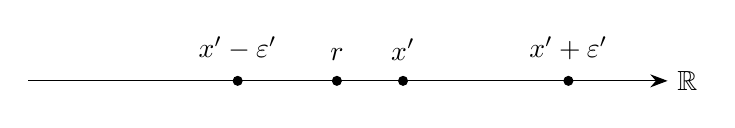
\begin{tikzpicture}[x=1.4cm]
    \draw[-{Stealth[length=2.2mm]}] (-0.4,0) -- (5.4,0) node[right] {$\mathbb{R}$};
    \foreach \p/\lbl in {1.5/{x'-\ep'}, 3/{x'}, 2.4/{r}, 4.5/{x'+\ep'}}
        \filldraw (\p,0) circle (1.6pt) node[above=4pt] {$\lbl$};
    \end{tikzpicture}
    \end{center}


    Then, we take $y = \sqrt{2} r$. 
    \begin{align*}
        |x - \sqrt{2} r| &= \sqrt{2} |x^{\prime} - r| \\
        & < \sqrt{2} \epsilon^{\prime} \\
        & = \epsilon
    \end{align*}

    \item 
Now we show (1), i.e. $\mathbb{Q}$ is dense in $\mathbb{R}$. 
I.e. WTS $\forall x \in \mathbb{R}, \forall \ep > 0$
$\exists y \in \mathbb{Q}$ s.t. 
$|x - y | < \ep$. 
\medskip 

By Archimedean property, $\exists n \in \mathbb{N} \text{s.t.} n \ep > 1$
\medskip

\begin{center}
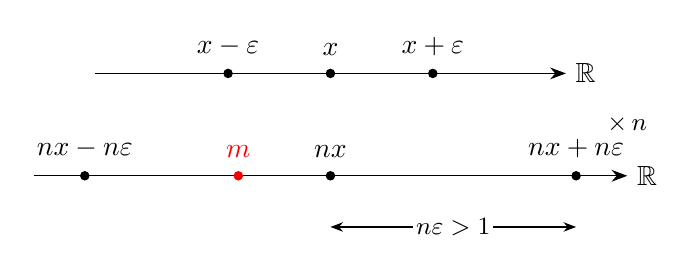
\begin{tikzpicture}[x=1.3cm]
  % original scale
  \draw[-{Stealth[length=2mm]}] (-2.3,1.3) -- (2.3,1.3) node[right] {$\mathbb{R}$};
  \foreach \p/\lbl in {-1/{x-\ep}, 0/{x}, 1/{x+\ep}}
    \filldraw (\p,1.3) circle (1.5pt) node[above=3pt] {$\lbl$};

  \node[font=\small] at (2.9,0.65) {$\times\, n$};

  % blown up by n
  \draw[-{Stealth[length=2mm]}] (-2.9,0) -- (2.9,0) node[right] {$\mathbb{R}$};
  \foreach \p/\lbl in {-2.4/{nx-n\ep}, 0/{nx}, 2.4/{nx+n\ep}}
    \filldraw (\p,0) circle (1.5pt) node[above=3pt] {$\lbl$};
  \filldraw[red] (-0.9,0) circle (1.5pt) node[above=3pt] {$m$};
  \draw[{Stealth[length=1.6mm]}-{Stealth[length=1.6mm]}] (0,-0.65) --
    node[fill=white,inner sep=1pt,font=\small] {$n\ep>1$} (2.4,-0.65);
\end{tikzpicture}
\end{center}



Also $
\forall y \in \mathbb{R}, \exists m \in \mathbb{Z}
\text{s.t.} |y - m| < 1
$ 
Hence take $y = nx$
\begin{align*}
& |nx - m | < 1 < n \ep \\
\implies & \left| x - \frac{m}{n} \right|  < \frac{n \ep}{n} = \ep
\end{align*}
    \end{enumerate}
\end{proof}

\newpage

\phantomsection
\section*{Side note: Cardinality}
\addcontentsline{toc}{section}{Side note: Cardinality}

\begin{definition}[Finite]
    A set $S \neq \emptyset$ is \textbf{finite}
    if $\exists n \in \mathbb{N}$
    and a bijection 
    $f: S \to \{ 1, 2, \hdots n \} $. 
    Otherwise $S$ is \textbf{infinite}.
\end{definition}

\begin{definition}[Countability]
    \hfill
    \begin{enumerate}
        \item A set $S$ is 
\textbf{countably infinite}
if there is a bijection $f: S \to \mathbb{N}$
        \item A set $S$ is \textbf{countable} 
if it is empty
or countably infinite 
        \item A set $S$ is \textbf{uncountable} if
it is not countable.
    \end{enumerate}
\end{definition}

\begin{remark}
    Every nonempty finite subset of $\mathbb{R}$ has a max and min. 
\end{remark}

\begin{proposition}
    \hfill 
    \begin{enumerate}
        \item Any subset of a countable set is countable.
        \item A countable union of countable sets is countable.
        \item $\mathbb{Q}$ is countable. \textbf{Exercise}
        \item $\mathbb{R} \setminus \mathbb{Q}$ is uncountable $\iff$ $\mathbb{R}$ is uncountable. \textbf{Exercise}
        \item Union of a countable set and an uncountable set is uncountable. 
    \end{enumerate}
\end{proposition}

\begin{proof}[Proof that $\mathbb{Q}$ is countable]
    There is an injection from $\mathbb{Q}$  to the set $A \coloneq \{ (a, b): a, b \in \mathbb{Z} \} $. 
    Fix arbitrary $a \in \mathbb{Z}$, $A_a \coloneq \{ (a, b) : b \in \mathbb{Z} \} $. There is a bijection 
    between $A_a$ and $\mathbb{Z}$, and $\mathbb{Z}$ countable, hence $A_a$ is countable. 
    $A = \bigcup_{a \in \mathbb{Z}}A_a$ is a countable union of countable sets and is therefore countable.
\end{proof}

\newpage 

\section{Metric spaces and point-set topology}

\subsection{Metric spaces, open and closed sets}

\begin{definition}[Metric space]
    A \textbf{metric space} $(X, d)$ is a set $X$
    of elements (called points)
    equipped with a metric or function
    $d: X \times X \to [0, \infty)$ 
    such that 
    \begin{enumerate}
        \item $\forall x, y \in X, d(x,y) \geq 0$. 
i.e. The image of $d$ is in $\mathbb{R}$ and non-negative 
        \item $d(x,y) = 0 \iff x = y$
        \item $\forall x, y \in X, d(x,y) = d(y,x)$
        \item $\forall x, y, z, \in X$, 
$d(x,z) \leq d(x, y) + d(y, z)$
    \end{enumerate}
\end{definition}

\begin{definition}[Discrete metric]
    The \textbf{discrete metric} $d$ is defined such that $\forall x, y$
    \[
        d(x,y) = \mathbf{1}[x \neq y] = 
        \begin{cases}
            0, \text{ if } x = y \\
            1, \text{ if } x \neq y 
        \end{cases}
    \]
\end{definition}


\begin{example}
    The following are metric spaces 
    \begin{itemize}
        \item $X = \mathbb{R}, d(x,y) = |x-y|$
        \item 
$
    X = \mathbb{R}^n := \{ 
        (x_1, x_2, \hdots x_n) : x_i \in \mathbb{R}
    \} 
$, 
$
d_1(x, y) = \left( \sum\limits_{i = 1}^{n} |x_i - y_i|^2 \right)^{ \frac{1}{2}}
$, i.e. Euclidean distance
        \item 
$
    X = \mathbb{R}^n 
$, 
$
d_2(x, y) = \max_i |x_i - y_i|
$
\item $X$ is the set of continuous functions on $[a, b]$, and $d(f,g) = \sup_{x \in [a, b]} |f(x) - g(x)|$
\item Any $X \neq \emptyset$ with the discrete metric.
    \end{itemize} 
\end{example}

\begin{definition}[Neighborhood]
    Let $(X,d)$ be a metric space. 
    Let $x \in X, \ep> 0$. 
    The \textbf{$\ep$-neighborhood} of $x$ 
    is 
    \[
        N(x, \ep) = B_{\ep}(x) := 
        \{ 
            y \in X, d(x, y) < \ep
        \} 
    \]
    A \textbf{deleted neighborhood} is 
    \begin{align*}
        N^{*}(x, \ep) :&= \{ 
            y \in X, 0 < d(x, y) < \ep
        \} \\
        &= N(x, \ep) \setminus \{ x \} 
    \end{align*}
\end{definition}

\begin{definition}[Interior]
    Let $(X, d)$ be a metric space, 
    $S \subset X$. 
    A point $x \in S$ is an 
    \textbf{interior point}  of $S$ if 
    \[
    \exists \ep > 0 
    \text{ s.t. }
    N(x, \ep) \subset S 
    \]

    I.e. If an $\ep$-neighborhood around $x$ 
    is in $S$, then $x$ is an interior point.

    \medskip
    
    The set of all interior points of $S$
    is called the \textbf{interior} of $S$, 
    denoted $\operatorname{int} S$
    \[
        \operatorname{int}  S := \{ 
        x \in S: \exists \ep > 0 \text{ s.t. }
        N(x, \ep) \subset S
        \} 
    \]
\end{definition}

\begin{definition}[Boundary]
    Let $(X, d)$ be a metric space, 
    $S \subset X$. 
    A point $x \in S$ is a \textbf{boundary point} of $S$ if 
    $\forall \ep > 0$,
    \begin{align*}
        N (x, \ep) \cap S \neq \emptyset \\
        N (x, \ep) \cap S^c \neq \emptyset
    \end{align*}
    The set of boundary pints of $S$ is $\operatorname{bd} S$
    \begin{align*}
        \operatorname{bd} S :&= \{ 
            x \in X: 
            \forall \ep > 0, 
            N(x, \ep) \cap S \neq \emptyset,
            N(x, \ep) \cap S^c \neq \emptyset
        \}  \\
        &= \left( \operatorname{int} S \cup \operatorname{int} S^c \right)^c
    \end{align*}
\end{definition}

\begin{example}
    $\operatorname{int} \mathbb{N} = \emptyset$, 
\end{example}
\begin{proof}
    Fix $x \in \mathbb{R}$ and $\varepsilon > 0$ arbitrary. 
    Take $y = x + \frac{1}{2} \min (\varepsilon, 1)$. Then 
    \begin{itemize}
        \item $|y - x| = \frac{1}{2} \min (\varepsilon, 1) \implies y \in N(x, \varepsilon)$
        \item $x < y < x + 1 \implies y \notin \mathbb{N}$ 
    \end{itemize} 
    Hence $N(x, \varepsilon) \not \subset \mathbb{N}$ for all $\varepsilon > 0 \implies x \notin \operatorname{Int}  \mathbb{N}$.
\end{proof}

\begin{example}
    $\operatorname{bd} \mathbb{N} = \mathbb{N}$.
\end{example}
\begin{proof}
    \begin{enumerate}
        \item $\mathbb{N} \subset \operatorname{bd}  N$.
Fix $x \in \mathbb{N}, \varepsilon > 0$, 
        \begin{itemize}
            \item 
$x \in N(x, \varepsilon) \cap \mathbb{N} \neq \emptyset$. 
            \item 
$y = x + \frac{1}{2} \min(\varepsilon, 1) \in N(x, \varepsilon) \cap \mathbb{N}^c \neq \emptyset$.
        \end{itemize} 
        \item $\mathbb{N} \supset \operatorname{bd}  N$. Fix arbitrary $x \in \operatorname{bd} \mathbb{N}$. 
ATC $x \notin \mathbb{N}$, then we consider 2 cases
\begin{itemize}
    \item if $x < 1$, then take $\varepsilon = 1 - x$. 
$\forall y \in N(x, \varepsilon), 1 > y \notin \mathbb{N}$, 
hence $N(x, \varepsilon) \cap \mathbb{N} = \emptyset$, 
which contradicts the definition of boundary point. 
    \item $if x > 1$, let $n \in \mathbb{N}$ such that 
$n < x < n + 1$. Let $\varepsilon = \frac{1}{2}\min(x - n, n + 1 - x)$, then 
$\forall y \in N(x, \varepsilon)$, $y \notin \mathbb{N}$, 
hence $N(x, \varepsilon) \cap \mathbb{N} = \emptyset$, 
which contradicts the definition of boundary point. 
\end{itemize} 
    \end{enumerate}
\end{proof}

\begin{remark}
    \hfill 
    \begin{enumerate}
        \item $\operatorname{int} S = S \setminus \operatorname{bd} S$
        \item boundary points may or may not be in $S$. 
        \item Any point in a set $S$ is either a boundary or an interior point, but not both.
    \end{enumerate}
\end{remark}



















%==============================================================================
% MATH 5080 — Introduction to Analysis I (Fall 2026)
% Class:        4
% Date:         Sept 3rd
%==============================================================================

\begin{definition}[Closure]
    The \textbf{closure} of $S$, denoted $\overline{S}$, is defined as 
    \[
    \overline{S} := S \cup \operatorname{bd}  S
    \]
\end{definition}

\begin{definition}[Openess and closedness]
    \hfill
    \begin{enumerate}
        \item $S \subset X$ is called \textbf{open} if $S = \operatorname{int} S$
        \item $S \subset X$ is called \textbf{closed} if $S^c$ is open.
    \end{enumerate}
\end{definition}

\begin{remark}
    A point cannot be both an interior point and a boundary point.
\end{remark}

\begin{remark}
    A set can be both open and closed. For example 
    \begin{itemize}
        \item $\mathbb{R}$ is both open and closed.
        \item $\emptyset$ is both open and closed.
        \item $\mathbb{N}$ is not open, but closed.
    \end{itemize} 
\end{remark}

\begin{example}
    $S = (1, 3)$ is open and not closed.
\end{example}

\begin{example}
    Let $(X, \sigma)$ be a metric space where $\sigma$ is the discrete 
    metric. Take $x_0 \in X$, $S = \{ x_0 \} $ is open. 
    \medskip 

    To see why, let $\ep = \frac{1}{2}$. 
    \begin{align*}
        & N \left(x_0, \frac{1}{2} \right) = \{ x_0 \}  \subset S \\
        \implies & x_0 \in \operatorname{int}  S \\
        \implies & \operatorname{int}  S = S \\
        \implies & S \text{ open}
    \end{align*}
    Hence any point in a set is interior, and any set is open and closed.
\end{example}

\begin{proposition}
    \hfill
    \begin{enumerate}
        \item $S$ open $\iff$ $\operatorname{bd} S \subset S^c$
        \item $S$ closed 
$\iff \operatorname{bd} S \subset S$
$\iff S = \overline{S} := S \cup \operatorname{bd} S$ 
        \item $\overline{S}$ is closed
        \item $\operatorname{int} S$ is open $\implies \operatorname{int} \left( \operatorname{int} (S)  \right) = \operatorname{int}(S)  $
    \end{enumerate}
\end{proposition}

\begin{proof}[Proof. $S$ closed $\iff$ $\operatorname{bd} S \subset S$]
    \hfill

    By definition, $S$ closed $\iff$ $S^c$ open. 
    Also by definition, $\operatorname{bd} S = \operatorname{bd} S^c$.
    \begin{align*}
        \operatorname{bd} S \subset S & \iff \operatorname{bd} S^c \subset S && \text{ by definition} \\
        & \iff \operatorname{bd} S^c \cap S^c = \emptyset \\
        & \iff \forall x \in S^c, x \notin \operatorname{bd} S^c \\
        & \iff \forall x \in S^c, x \in \operatorname{int} S^c \\
        & \iff S^c = \operatorname{int} S^c \\
        & \iff S^c \text{ open} \\
        & \iff S \text{ closed}
    \end{align*}
\end{proof}

\begin{proposition}
    \hfill
    \begin{enumerate}
        \item The union of open sets is open.  
        \item The intersection of finitely many open sets is open.
    \end{enumerate}
    \remind{Add in analogous propositions about closed sets.}
\end{proposition}

\begin{example}
    $S_n = \left( - \frac{1}{n}, \frac{1}{n} \right) $ is open for all $n \in \mathbb{N}$. 
    $\bigcap_{n=1}^{\infty} S_n = \{ 0 \} $ is closed. 

    \medskip 

    To see why the intersection is closed, 
    $\forall x >0$, by AP, $\exists n \in \mathbb{N}$ 
    s.t. $0 < \frac{1}{n} < x$. 
    Hence $x \notin S_n$ and 
    $S \notin \bigcap S_n$. 
    \medskip

    At the same time, $0 \in S_n, \forall n \in \mathbb{N}$. 
    \medskip

    Since $0 \notin \operatorname{int} \{ 0 \}  $, $\{ 0 \} $ is not open.
\end{example}

\begin{proof}[Proof of 3.9.2]
    WTS intersection of finitely many open sets is open. 
    \medskip

    Let $S_1, \hdots S_n$ be open sets, $S = \bigcap_{k = 1}^n S_k$. 
    WTS $\forall x S, \exists \ep \in \mathbb{R}, \ep > 0$
    s.t. 
    $N(x , \ep) \subset S$. 
    Note that 
    \[
        N(x, \ep ) \subset S \iff
        N(x, \ep ) \subset S_i, \forall i = 1, \hdots, n
    \]
    Since $x \in S_i$ and $S_i$ is open, $\exists \ep_i > 0$ s.t. 
    $N(x, \ep_i) \subset S_i$. 
    Let $\ep = \min \{ \ep_1, \hdots, \ep_n  \} $,
    and we know such $\ep$ exists 
    because a sequence of finitely many numbers has a minimum.
\end{proof}

\begin{definition}[Accumulation points and isolated points]
    \hfill 
    \begin{enumerate}
        \item
    Let $S \subset X$, a point $x \in X$ is an \textbf{accumulation point}
    of $S$ if $\forall \ep > 0$, 
    \[
        N^*(x, \ep) \cap S \neq \emptyset
    \]
    The set of all accumulation points of $S$ is denoted $S^{\prime}$.
        \item If $x \in S \setminus S^{\prime}$, then $x$ is an 
\textbf{isolated point} of $S$.
    \end{enumerate}
\end{definition}

\begin{example}
    $S = \{ 0 \}  \cup (1, 2)$, $S^{\prime} = [1, 2]$
\end{example}

\begin{example}
    $S = \mathbb{Q} \cap (1, 2)$, $S^{\prime} = [1, 2]$
\end{example}

\begin{proposition}\label{prop:closure-acc}
    \hfill
    \begin{enumerate}[ref=\theproposition.\arabic*]
        \item\label{prop:closure-acc-1} $\overline{S} = S \cup S^{\prime}$
        \item\label{prop:closure-acc-2} $S$ close $\iff S^{\prime} \subset S$
        \item\label{prop:closure-acc-3} $\overline{S}$ is the smallest closed set that contains $S$.
    \end{enumerate}
\end{proposition}

\begin{proof}[Proof of \ref{prop:closure-acc-1}]
    WTS $S \cup \operatorname{bd} S = S \cup S^{\prime}$. 
    \begin{enumerate}
        \item We first show that $LHS \subset RHS$. 
$\forall x \in S \cup \operatorname{bd} S$, $x \in S \cup S^{\prime}$. 
\medskip 

If $x \in S$, done. 
\medskip

If $x \in \operatorname{bd} S$, $x \notin S$ then $x \in \operatorname{bd} S \cap S^c$. 
WTS $x \in S^{\prime}$, i.e. $\forall \ep > 0, N^*(x, \ep) \neq \emptyset$. 
\medskip 

Since $x \in \operatorname{bd} S$, we know $N(x, \ep) \cap S \neq \emptyset$. 
Since $x \in S^c$, we know $\exists y \in N(x, \ep)\cap S, y \neq x$. 
Hence $y \in N^*(x, \ep) \cap S$, 
and $N^*(x, \ep) \neq \emptyset$.
\item We then show $RHS \subset LHS$, i.e. 
$\forall x \in S \cup S^{\prime}, x \in S \cup \operatorname{bd} S$. 
\medskip 

If $x \in S^{\prime}$, done. 
\medskip 

If $x \in S^{\prime}, x \notin S$, $x \in S^{\prime} \cap S^c$, 
WTS $x \in \operatorname{bd} S$
\remind{Exercise}.
    \end{enumerate}
\end{proof}












%==============================================================================
% MATH 5080 — Introduction to Analysis I (Fall 2026)
% Class:        5
% Date:         Sept 8th
%==============================================================================

\begin{theorem}[Bolzano-Weiestrass]
    If $S \subset \mathbb{R}$ is bounded and contains infinitely many points then $S^{\prime} \neq \emptyset$.
\end{theorem}

\begin{remark}
    Bolzano-Weierstrass gives the existence of limit points, but it does not tell us 
    that the limit points are in $S$. 
\end{remark}

\begin{proof}
    Suppose $S^{\prime} = \emptyset$, then $S = \bar{S} $ is closed. 
    By HB, $S$ is compact.
    \medskip 

    For any $x \in S, x \notin S^{\prime}$, $x$ must be isolated point, i.e. 
    \[
        \exists \ep_x > 0, s.t. N(x, \ep_x) \cap S = \{ x \} 
    \]
    Then $ \{ N(x, \varepsilon_x) \}_{x \in S} $ is an open cover of $S$. 
    By compactness, $\exists x_1, x_2, \hdots x_N$ s.t. 
    \[
        N(x_1, \varepsilon_{x_1}) \cup \hdots N(x_N, \varepsilon_{x_N}) \supset S
    \]
    However, each one of the neighborhoods contains only its center, i.e. 
    \[
        N(x_1, \varepsilon_{x_1}) = \{ x_1 \}, \hdots N(x_n, \varepsilon_{x_N}) = \{ x_N \} 
    \]
    Hence 
    \[
        \{ x_1 \}  \cup \hdots \{ x_N \}  \supset S
    \]
    and this contradicts $S$ having infinitely many points.
\end{proof}

\begin{remark}
    $S$ has infinite points and $S^{\prime} \neq \emptyset \not \implies S$ bounded. 
\end{remark}

\begin{proof}
    Let $S \coloneq [1, 2] \cup \mathbb{N}$.
    Then $S^{\prime} = [1, 2] \neq \emptyset$  , but $S$ unbounded.
\end{proof}

\begin{remark}
    If $S \subset \mathbb{R}$, and every 
    infinite subset of $\mathbb{S}$ has an accumulation point in $\mathbb{R}$, 
    then $S$ is bounded.
\end{remark}

\begin{proof}
    \remind{To be added in}
\end{proof}

\begin{remark}[Relationship between results]
    \hfill
    \begin{center}
    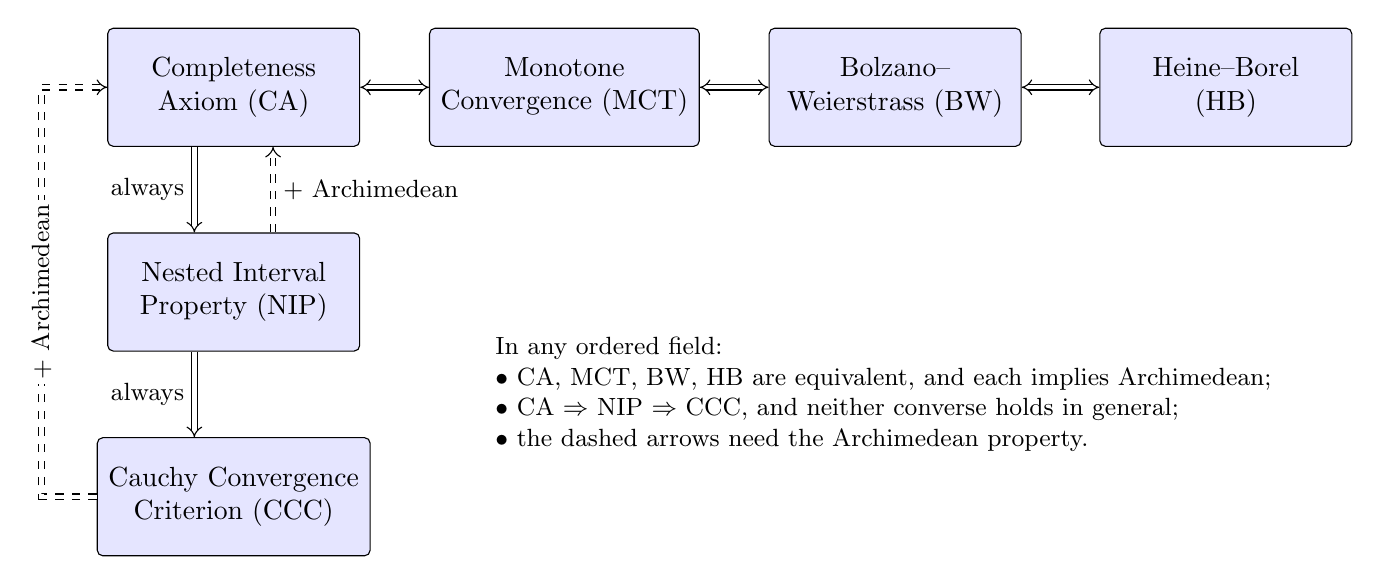
\begin{tikzpicture}[
        thm/.style={
            draw, 
            rounded corners=2pt, 
            fill=blue!10, 
            minimum height=1.5cm,
            minimum width=3.2cm,
            align=center,
            inner sep=4pt
        },
        imp/.style={
            double,
            double distance=1.6pt,
            -{Implies[length=2.6mm]}
        },
        eqv/.style={
            double,
            double distance=1.6pt,
            {Implies[length=2.6mm]}-{Implies[length=2.6mm]}
        },
        lbl/.style={font=\small, fill=white, inner sep=1.5pt}
    ]
        \node[thm] (CA)  at (0,0)    {Completeness\\Axiom (CA)};
        \node[thm] (MCT) at (4.2,0)  {Monotone\\Convergence (MCT)};
        \node[thm] (BW)  at (8.4,0)  {Bolzano--\\Weierstrass (BW)};
        \node[thm] (HB)  at (12.6,0) {Heine--Borel\\(HB)};
        \node[thm] (NIP) at (0,-2.6) {Nested Interval\\Property (NIP)};
        \node[thm] (CCC) at (0,-5.2) {Cauchy Convergence\\Criterion (CCC)};

        \draw[eqv] (CA) -- (MCT);
        \draw[eqv] (MCT) -- (BW);
        \draw[eqv] (BW) -- (HB);
        \draw[imp] ([xshift=-0.5cm]CA.south) -- node[lbl, left=2pt] {always} ([xshift=-0.5cm]NIP.north);
        \draw[imp] ([xshift=-0.5cm]NIP.south) -- node[lbl, left=2pt] {always} ([xshift=-0.5cm]CCC.north);
        \draw[imp, dashed] ([xshift=0.5cm]NIP.north) -- node[lbl, right=2pt] {+ Archimedean} ([xshift=0.5cm]CA.south);
        \draw[imp, dashed] (CCC.west) -- ++(-0.7,0) |- node[lbl, pos=0.25, rotate=90] {+ Archimedean} (CA.west);

        \node[font=\small, align=left, anchor=west] at (3.2,-3.9) {
            In any ordered field:\\
            $\bullet$ CA, MCT, BW, HB are equivalent, and each implies Archimedean;\\
            $\bullet$ CA $\Rightarrow$ NIP $\Rightarrow$ CCC, and neither converse holds in general;\\
            $\bullet$ the dashed arrows need the Archimedean property.
        };
    \end{tikzpicture}
    \end{center}
\end{remark}


%==============================================================================
% MATH 5080 — Introduction to Analysis I (Fall 2026)
% Class:        6
% Date:         Sept 10th
%==============================================================================

\begin{theorem}
    [Nested Interval Property]
    \label{thm:NIP}
    Let $\{ I_n = [a_n, b_n]: n \in \mathbb{N} \} $ be a family of closed 
    bounded intervals s.t. $I_{n + 1} \subset I_n$ and $I_n \neq \emptyset$,
    $\forall n \in \mathbb{N}$. Then 
    \[
        \bigcap_{i = 1}^{\infty} I_n \neq \emptyset
    \]
\end{theorem}

\begin{theorem}[Generalized NIP]
    \label{thm:generalized-NIP}
    If $\mathcal{F} = \{ K_{\alpha} \} $ is a collection of compact 
    subsets of $X$ such that the intersection of every finite 
    subcollection of $\mathcal{F}$ is nonempty, then 
    \[
        \bigcap_{\alpha} K_{\alpha} \neq \emptyset
    \]
\end{theorem}

\begin{remark}[Theorem \ref{thm:generalized-NIP} $\implies$ theorem \ref{thm:NIP}]
    \hfill
    Let $\mathcal{F} = \{ I_n : n \in \mathbb{N} \}$ be as in Theorem \ref{thm:NIP},
    with $X = \mathbb{R}$. We check the hypotheses of Theorem \ref{thm:generalized-NIP}.
    \medskip

    \textbf{Compactness.} Each $I_n = [a_n, b_n]$ is closed and bounded in $\mathbb{R}$,
    hence compact by Heine-Borel.
    \medskip

    \textbf{Finite intersections are nonempty.} Take any finite subcollection
    $I_{n_1}, \hdots, I_{n_k}$ and let $N = \max\{ n_1, \hdots, n_k \}$.
    Since the intervals are nested, $I_m \subset I_n$ whenever $m \geq n$, so
    $I_N \subset I_{n_j}$ for every $j$. Therefore
    \[
        I_{n_1} \cap \hdots \cap I_{n_k} = I_N \neq \emptyset
    \]
    by assumption.
    \medskip

    Hence Theorem \ref{thm:generalized-NIP} applies and gives
    \[
        \bigcap_{n = 1}^{\infty} I_n \neq \emptyset
    \]
\end{remark}

\begin{proof}[Proof of \ref{thm:generalized-NIP}]
    Suppose $\bigcap_{\alpha}K_{\alpha} = \emptyset$. 
    Fix any $K_{\alpha_0} \in \mathcal{F}$. 
    $K_{\alpha_0}$ is compact by assumption. 
    Fix $x \in K_{\alpha_0}$. 
    \begin{align*}
        x \notin \bigcap_{\alpha}K_{\alpha} & 
        \implies \exists \alpha_x \text{ s.t. } x \notin K_{\alpha_x} 
        \iff x \in K_{\alpha_x}^c 
    \end{align*}
    Also 
    $K_{\alpha_x}$ compact $\implies$
    $K_{\alpha_x}$ closed $\implies$
    $K_{\alpha_x}^c$ open. 
    Hence $\{ K_{\alpha_x} \}_{x \in K_{\alpha_0}} $ is an open cover 
    of $K_{\alpha_0}$. 
    By compactness of $K_{\alpha_0}$, $\exists \alpha_1, \hdots \alpha_N$
    s.t. 
    \begin{align*}
        & K_{\alpha_0} \subset K_{\alpha_1}^c \cup \hdots K_{\alpha_N}^c \\
        \iff & K_{\alpha_0} \cap ( K_{\alpha_1}^c \cup \hdots K_{\alpha_N}^c)^c = \emptyset \\
        \iff & K_{\alpha_0} \cap  K_{\alpha_1} \cap \hdots K_{\alpha_N} = \emptyset
    \end{align*}
    which contradicts the assumption that any finite subcollection has a 
    nonempty intersection.
\end{proof}

\subsection{Connected sets}

\begin{definition}[Disconectedness / connectedness]
    A set $S \subset X$ is \textbf{disconnected} if 
    $\exists A, B$ s.t. 
    \begin{itemize}
        \item $A, B$ open 
        \item $S \subset A \cup B$
        \item $A \cap S \neq \emptyset$
        \item $B \cap S \neq \emptyset$
        \item $A \cap B = \emptyset$
    \end{itemize} 
\end{definition}

\begin{example}
    \hfill 
    \begin{enumerate}
        \item $(1, 2) \cup (2, 3)$ disconnected, 
        take $A = (0, 2), B = (2, \infty)$
        \item $\mathbb{Q}$ disconnected, 
        take $A = (-\infty, \sqrt{2}), B = (\sqrt{2}, \infty)$
        \item For a discrete metric space, 
        connected sets are $\emptyset$ or singleton, 
        any other set is disconnected.
        \item Any singleton set is connected.
    \end{enumerate}
\end{example}

\begin{definition}
    A set $S \subset \mathbb{R}$ is an \textbf{interval} if 
    $\forall a, b \in \mathbb{R}, a < b$
    \[
        a \in S, b \in S \implies [a, b] \subset S
    \]
\end{definition}

\begin{theorem}[Connected sets in $\mathbb{R}$]
    \label{theorem:connected-sets-in-R}
    $S \subset \mathbb{R}$ is connected 
    if and only if one of the following holds
    \begin{enumerate}
        \item $S = \emptyset$ 
        \item $S$ singleton
        \item $S$ is an interval.
    \end{enumerate}
\end{theorem}

\begin{proof}
    \begin{enumerate}
        \item $\implies$: 
            Assume $S \subset \mathbb{R}$ connected and contains 
            at least 2 points. 
            WLOG, $a < b, a \in S, b \in S$. 
            WLOG, assume $\inf S, \sup S \notin S $. 
            WTS $S = (\inf S, \sup S)$.
            \begin{itemize}
                \item $S \subset (\inf S, \sup S)$ is for free. 
                \item Suffices to show $(\inf S, \sup S) \subset S$
                \medskip 

                Suppose $\exists x \in (\inf S, \sup S) \cap S^c$, 
                then let $A \coloneq (\infty, x), B = (x, \infty)$. 
                Then
                \begin{itemize}
                    \item $S \subset A \cup B$
                    \item $A \cap B = \emptyset$
                    \item $A, B$ open 
                    \item $A \cap S \neq \emptyset$ because by definition of 
                    infimum, $\exists y \in S$ s.t. 
                    $\inf S < y < x$
                    \item $B \cap S \neq \emptyset$ because $\exists y \in S$
                    s.t. $\sup S > y > x$.
                \end{itemize} 
            \end{itemize} 
            \item $\impliedby$ 
            \label{proof:connected-sets-in-R}
    \end{enumerate}
\end{proof}

\begin{definition}[Separatedness]
    Two sets $A,B \subset X$ are \textbf{separated} if 
    \[
        \bar{A}  \cap B = \emptyset, A \cap \bar{B}  = \emptyset
    \]
\end{definition}

\begin{remark}
    $A, B$ separated may not necessarily have $\bar{A} \cap \bar{B}  = \emptyset$,
    e.g. 
    \[
        A = (0, 1), B = (1, 2)
    \]
\end{remark}
\begin{remark}
    \begin{itemize}
        \item Separate $\implies$ Disjoint 
        \item Separate $\not \impliedby$ Disjoint, e.g. 
        \[
        A = (0, 1], B = (1, 2)
        \]
    \end{itemize} 
\end{remark}

\begin{definition}[Relatively open / closed sets]
    Let $S \subset X$, a set $E \subset S$ is 
    \textbf{relatively open} in $S$ if there is an open set $U \subset X$
    s.t. $E = S \cap U$. 
    \medskip 

    $E$ is \textbf{relatively closed} in $S$ 
    if there is a closed set $U \subset X$
    s.t. $E = S \cap U$.
\end{definition}

\begin{theorem}
    Let $S \subset X$, TFAE 
    \begin{enumerate}
        \item $S$ is disconnected 
        \item $\exists$ nonempty sets $A, B \subset S$ s.t. $A, B$ relatively 
        open in $S$, $A \cap B = \emptyset, S = A \cup B$.
        \item $\exists $ nonempty sets $A, B \subset S$ s.t. $A, B$ separated, and 
        $S = A \cup B$
    \end{enumerate} 
\end{theorem}


\newpage

\section{Numerical Sequences}

\begin{definition}[Sequence]
    A \textbf{sequence} $\{ a_n: n \in \mathbb{N} \}$
    $= \{ a_1, a_2, \hdots a_n, \hdots \} $ is a function 
    $f: \mathbb{N} \to \mathbb{R}$.
\end{definition}

\subsection{Convergent sequences}

\begin{definition}[Convergence]
    A sequence $\{ a_n \} $ \textbf{converges}
    to $L \in \mathbb{R}$ if $\forall \varepsilon > 0$, 
    $\exists N > 0$ s.t. $\forall n > \mathbb{N}$
    \[
        |a_n - L | < \varepsilon
    \]
    Then we say that $L$ is the \textbf{limit} of $\{ a_n \} $, and denote 
    \[
        \lim_{n \to \infty} a_n = L
    \]
    If $\{ a_n \} $ doesn't converge to any real number, we say $ \{ a_n \} $ \textbf{diverges}.
\end{definition}

\begin{example}
    $\{ (-1)^n \} $ diverges.
\end{example}

\begin{proof}
    Suppose $\lim_{n \to \infty}a_n = L$. 
    Let $\varepsilon = \frac{1}{100}$. 
    Then either $1$ or $-1$ is not in $N(L, \varepsilon)$.
\end{proof}

\begin{theorem}[Uniqueness of limit]
    If a sequence converges then the limit is unique.
\end{theorem}

\begin{proof}
    ATC otherwise, then $\{ a_n \} $ converges to two different limits,
    $L_1 \neq L-2$. 
    Let $\ep = \frac{1}{3} \left| L_1 - L_2 \right|  > 0$> 
    By definition of limit, 
    \begin{itemize}
        \item $\exists N_1 > 0$ s.t. $\forall n > N_1, |a_n - L_1| < \ep$
        \item $\exists N_2 > 0$ s.t. $\forall n > N_2, |a_n - L_2| < \ep$
    \end{itemize} 
    Then let $n > \max \{ N_1, N_2 \} $, then $|a_n - L_1| < \ep, |a_n - L_2| < \ep$, 
    and 
    \begin{align*}
        |L_1 - L_2| &= |L_1 - a_n + a_n - L_2 |  \\
        & \leq  |L_1 - a_n| + |a_n - L_2| \\
        & < 2 \ep \\
        &= \frac{2}{3} |L_1 - L_2| 
    \end{align*}
\end{proof}

\begin{theorem}[Convergence implies bounded]
    If a sequence converges then it is bounded.
\end{theorem}

\begin{proof}
    \textit{
        The idea is that if a sequence converges to $L$, 
        past a certain point, everything is close to $L$.
        We only have to deal with finitely many terms 
        before the sequence gets close to $L$,
        in which case we can take a max.
    }


    Assume $\lim_{n \to \infty}a_n = L$, and let $\varepsilon = 1$. 
    Then $\exists N \in \mathbb{N}$ s.t. $|a_n - L| < 1, \forall n > N$. 
    Hence, $\forall n \geq N$
    \begin{align*}
        |a_n| &= |a_n - L + L |  \\
        & \leq |a_n - L| + |L| \\
        & < 1 + |L|
    \end{align*}
    \medskip

    Let $M \coloneq \max \{ |a_1|, |a_2|, \hdots |a_N|, |L| + 1 \} $. 
    Then $ |a_n| \leq M, \forall n > N$.
\end{proof}

\begin{proposition}[Limits and accumulation points]
    \hfill
    \begin{enumerate}
        \item If $\lim_{n \to \infty} a_n = L$ and if $\{ a_n \} $
        attains infinitely many values, then $L$ is an accumulation point of $ \{ a_n \} $.
        \item If $L \in S^{\prime}$ then $S$ contains a sequence 
        $\{ a_n \} $ that converges to $L$.
    \end{enumerate}
\end{proposition}
\begin{proof}
    \begin{enumerate}
        \item \textit{$a_n \to L \implies N(L, \ep)$ contains all but finitely many terms.}
        Fix $\varepsilon > 0$. WTS $\exists x \in \{ a_n \} \cap N^*(L, \varepsilon)$
        Since $\lim_{n \to \infty} a_n = L, \exists N > 0$ 
        s.t. $a_n \in N(L, \varepsilon), \forall n > N$.
        \medskip 

        ATC otherwise, then $a_n = L, \forall n > N$. Then
        $\{ a_n \} $ contains only $a_1, a_2, \hdots, a_N, L$, 
        which contradicts the assumption that $\{ a_n \} $
        has infinitely many values.
        \item Let $\varepsilon_1 = 1$. Since $L$ is an accumulation point,
        \begin{align*}
            L \in S^{\prime} & = \implies \exists a_1 \in S \cap N^*(L, \varepsilon_1)
        \end{align*}
        Repeat this, setting $\varepsilon_n = \frac{1}{n}$, and picking
        $a_n \in S \cap N^*(L, \varepsilon_n)$.
        \medskip 

        We claim that $\lim a_n = L$. Fix any $\varepsilon > 0$,
        by AP, $\exists N \in \mathbb{N}$ s.t. $ \frac{1}{N} < \varepsilon$, 
        then $\forall n > N$, 
        \[
            |a_n - L| < \frac{1}{n} < \frac{1}{N} < \varepsilon
        \]
    \end{enumerate}
\end{proof}

\begin{remark}
    If $ \{ a_n \} $ has infinitely many values, $a_n \to L$, then $L$ is \textbf{unique} the accumulation point. 
\end{remark}










%==============================================================================
% MATH 5080 — Introduction to Analysis I (Fall 2026)
% Class:        7
% Date:         Sept 15th
%==============================================================================

\begin{theorem}[Operation on limits]
    Suppose 
    $\lim_{n \to \infty} a_n = A$,
    $\lim_{n \to \infty} b_n = B$, then 
    \begin{enumerate}
        \item $\lim_{n \to \infty}(a_n + b_n) = A + B$
        \item $\lim_{n \to \infty}ka_n = kA$
        \item $\lim_{n \to \infty}a_n b_n = AB$
        \item If $b_n \neq 0, \forall n$ and $B \neq 0$, then 
        \[
            \lim_{n \to \infty} \frac{a_n}{b_n} = \frac{A}{B}
        \]
    \end{enumerate}
\end{theorem}

\begin{proof}[Proof of 3]
    \textit{
        The idea is to use boundedness of one of the sequences to 
        find a bound on the deviation for each of the convergent sequences
        from their limits, and then take the bigger $N$.
    }
    \medskip

    Fix $\ep > 0$, seek $N > 0$ s.t. $\forall n > N, \left| a_n b_n - AB \right| < \ep $.
    \begin{align*}
        \left| a_n b_{n} - AB \right|  
        &= \left| a_{b}b_{n} - a_{b}B + a_{b}B - AB \right| \\
        &\leq \left| a_{n}b_{n} - a_{n}B \right| + \left| a_{n}B - AB \right| \\
        &= \left| a_{n} \right|  |b_{b} - B| + |a_{n} - A | |B|
    \end{align*}
    Since convergent implies boundedness, $\exists M > 0$ s.t. $| a_n | \leq M, \forall n$.
    Choose $M$ such that $|B| \leq M$. 
    \medskip

    By convergence of $a_n, b_n$, we can choose
    \begin{itemize}
        \item $N_1 > 0$ s.t. $|a_n - A | < \frac{\ep}{2M}, \forall n > N_1$
        \item $N_2 > 0$ s.t. $|a_n - A | < \frac{\ep}{2M}, \forall n > N_2$
        \item $N = \max \{ N_1, N_2 \} $
    \end{itemize} 
    Then $\forall n > N$
    \begin{align*}
        \left| a_n b_{n} - AB \right|  
        &\leq \left| a_{n} \right|  |b_{b} - B| + |a_{n} - A | |B| \\
        &< |a_n | \cdot \frac{\ep}{2M} + \frac{\ep}{2M} \cdot |B| \\
        & \leq \frac{\ep}{2} + \frac{\ep}{2} \\
        &= \ep
    \end{align*}
\end{proof}

\begin{example}
    $\lim_{n \to \infty} \frac{n + 1}{2n - 1} = \frac{1}{2}$ 
    \medskip

    By definition, fix $\ep > 0$, seek $N > 0$ s.t. $\forall n > N$, 
    \[
        \left| 
            \frac{n+1}{2n-1} - \frac{1}{2}
        \right|  < \ep
    \]
    Simplifying the expression, we get
    \begin{align*}
        & \left| 
            \frac{n+1}{2n-1} - \frac{1}{2}
        \right|  
        = \left| \frac{2n + 2 - 2n +1}{2(2-n-1)} \right| 
        = \frac{3}{2} \frac{1}{2n - 1} < \ep \\
        \iff &  \frac{1}{2n - 1} < \frac{2}{3}\ep \\
        \iff & 2n - 1 > \frac{3}{2} \ep \\
        \iff & n > \frac{1}{2} \left( \frac{3}{2} \ep  + 1 \right) 
    \end{align*}
    Take 
    \[
        N= 
        \lceil
        \frac{1}{2} \left( \frac{3}{2} \ep + 1 \right)
        \rceil
    \]
    and we are done. 

    \medskip

    Alternatively, \textit{we can prove using algebraic properties}.
    \begin{align*}
        \frac{n + 1}{2n - 1} 
        &= \frac{ \frac{1}{2} (2n-1) + \frac{3}{2}}{2n - 1} \\
        &= \frac{1}{2} + \frac{3}{2} \frac{1}{2n -1}
    \end{align*}
    It suffices to prove $\lim_{n  \to \infty} \frac{1}{2n-1} = 0$.
    Then by theorem, $\lim_{n \to \infty} \frac{n + 1}{2n-1} = \frac{1}{2} + \frac{3}{2} \cdot 0 = \frac{1}{2}$.
\end{example}


\begin{corollary}
    If $\lim_{n \to \infty}a_n$ converges, and $\lim_{n \to \infty} b_n$ diverges,
    then $\lim_{n \to \infty}a_n + b_n$ diverges.
\end{corollary}

\begin{example}
    Show $\lim_{n \to \infty} a^{ \frac{1}{n}} = 1$ 
    \medskip

    \textbf{Proof}
    We consider 3 cases
    \begin{itemize}
        \item $a < 1$: then by theorem,
        \begin{align*}
            &\lim_{n \to \infty} \frac{1}{a^{ \frac{1}{n}}}
            = \frac{1}{ \lim_{n \to \infty} a^{ \frac{1}{n}}} \\
            \implies & \lim_{n \to \infty} a^{ \frac{1}{n}} = 
            \frac{1}{\lim_{n \to \infty} \frac{1}{a^{ \frac{1}{n}}}}
            = \frac{1}{\lim_{n \to \infty} \left( \frac{1}{a} \right)^{ \frac{1}{n}} }
        \end{align*}
        and then we are in the case of $a > 1$
        \item $a = 1$: trivial
        \item $a > 1$
    \end{itemize} 

    Hence it suffices to show for $a > 1$. 
    Fix $\ep > 0$, we seek $N$ s.t. $\forall n > N$,
    \begin{align*}
        & \left| a^{ \frac{1}{n}} - 1 \right| < \ep \\
        \iff & a^{ \frac{1}{n}} - 1 < \ep \\
        \iff & a^{ \frac{1}{n}}  < 1 + \ep \\
        \iff & \frac{1}{n} \ln a < \ln( 1 + \ep) \\
        \iff & n > \frac{ \ln a}{\ln ( 1 + \ep)}
    \end{align*}
    Hence we can take 
    \[
        N = 
        \lceil
        \frac{\ln a}{\ln ( 1 + \ep)}
        \rceil
    \]
    and we are done.
\end{example}


\begin{theorem}[Sandwich Theorem]
    Let $N_0$ such that $a_n \leq c_n \leq b_n$,
    $\forall n > N_0$,
    suppose
    \[
        \lim_{n \to \infty} a_n =
        \lim_{n \to \infty} b_n = L
    \]
    then 
    \[
        \lim_{n \to \infty} c_n = L
    \]
\end{theorem}

\begin{proof}
    Fix $\varepsilon > 0$, we seek $N > 0$ s.t. $\forall n > N$,
    \[
        |c_n - L| < \varepsilon
    \]
    Since $\lim a_n = L, \exists N_1$ s.t. 
    $\forall n > N_1$,
    $|a_n - L | < \ep$
    Since $\lim b_n = L, \exists N_2$ s.t. 
    $\forall n > N_2$,
    $|b_n - L | < \ep$
    Pick $N = \max \{ N_1, N_2, N_0 \} $, 
    then $\forall n > N$,
    \begin{align*}
        c_n - L \leq b_n - L < \ep \\
        c_n - L \geq a_n - L > -\ep \\
    \end{align*}
    Hence 
    \[
        \left| c_n - L  \right|  < \ep
    \]
    
\end{proof}

\begin{example}
    Show $\lim_{n \to \infty} n^{ \frac{1}{n}} = 1$ 
    \medskip

    By sandwich theorem, we first have $n^{ \frac{1}{n}} \geq 1$
    for all $n \geq 1$. Hence we have found a lower bound 
    for all terms with $n > 1$.
    \medskip

    We then seek an upper bound that goes to 1. 
    Define a helper $h_n = n^{ \frac{1}{n}} - 1$,
    then $n^{ \frac{1}{n}} = 1 + h_n$. 
    We want to find an upper bound of $h_n$ that 
    goes to 0. 
    Write 
    \begin{align*}
        n^{ \frac{1}{n}} & = 1 + h_n \\
        \left( n^{\frac{1}{n}} \right)^{n} & = (1 + h_n)^n \\
        &= \sum\limits_{k = 0}^{n} 
        \begin{pmatrix} n \\ k \end{pmatrix} 
        h_n^k \\
        & \geq \begin{pmatrix} n \\2 \end{pmatrix} h_n^2 \\
        &= \frac{n(n-1)}{2} h_n^2 \\
        \frac{2n}{n(n-1)} &\geq h_n^2 \\
        \sqrt{ \frac{2}{n-1}} & \geq h_n
    \end{align*}
    Hence we can apply the sandwich theorem and say that 
    $n^{ \frac{1}{n}} \to 1$.
\end{example}

\begin{definition}[Divergence]
    We say $\{ a_n \} $ diverges to $\infty$ if $\forall M > 0$,
    $\exists N > 0$ s.t. $a_n > M, \forall n > N$, denoted 
    \[
        \lim_{n \to \infty} a_n = \infty
    \]
\end{definition}

\begin{example}
    $\{ 0, 2, 0, 4, \hdots \} $ does not diverge to $\infty$.
\end{example}

\subsection{Cauchy sequences and monotone sequences}

\begin{definition}[Cauchy sequence]
    $\{ a_n \} $ is a \textbf{Cauchy sequence} if $\forall \varepsilon > 0$, 
    $\exists N > 0$ s.t. $|a_n - a_m| < \varepsilon, \forall n, m > N$.
\end{definition}

\begin{theorem}[Cauchy implies boundedness]
    Every Cauchy sequence is bounded.
\end{theorem}
\begin{proof}
    Fix $\{ a_n \} $ a Cauchy sequence. 
    Fix $\varepsilon = 1$, by definition, 
    $\exists N_0 > 1$ s.t. $\forall n, m > N_0$,
    $|a_n - a_m| < 1$. 
    Hence, $a_n < |a_{N_0 + 1}| + 1, \forall n > N_0$. 
    \medskip 

    Also, $\{ a_n \}_{1 \leq n \leq N_0} $ is finite 
    and a maximum exists. 
    \medskip

    Hence $M \coloneq \max \{ 
        a_1, \hdots a_{N_0},
        |a_{N_0 + 1}|
    \} 
    $ bounds the whole sequence.
\end{proof}

\begin{theorem}[Convergence imply Cauchyness]
    Every convergent sequence is Cauchy.
\end{theorem}
\begin{proof}
    Fix sequence $ \{ a_n \} $, fix $ \varepsilon > 0$. Let limit be $L$. 
    Since $a_n$ converges, $\exists N > 0$ s.t. 
    \begin{align*}
        & |a_n - L | < \frac{\varepsilon}{2}, \forall n > N\\
        \implies & \forall n, m > N, |a_n - L| < \frac{\varepsilon}{2}, 
        |a_m - L | < \frac{\varepsilon}{2} \\
        \implies & |a_n - a_m| = 
        |(a_n - L) - (a_m - L)| \leq |a_n - L | + |a_m - L | < 
        \frac{\varepsilon}{2} + 
        \frac{\varepsilon}{2} = \varepsilon
    \end{align*}
\end{proof}


\begin{theorem}[Cauchy Convergence Criterion]
    If $\{ a_n \} \in \mathbb{R}$ is Cauchy then it 
    converges, and the limit is in $\mathbb{R}$. 
\end{theorem}

\begin{proof}
    \textit{We use Bolzano-Weierstrass to show existence of limit.}
    \medskip 

    Consider two cases. $\{ a_n \} $ is either finite or infinite. 
    \begin{itemize}
        \item $\{ a_n \} $ finite. Let $S$ dnote the set of values $ \{ s_1, \hdots s_k \} $. 
        Let $\varepsilon = \frac{1}{2} \min \{ |s_i - s_j| \}, i \neq j, 1 \leq i, j \leq k $. 
        \medskip 

        Since $\{ a_n \} $ is Cauchy, $\exists N > 0$ s.t. 
        \[
            |a_n - a_m| < \varepsilon, \forall n, m > N \implies 
            \exists i \text{ s.t. } a_n = s_i, \forall n > N
        \]
        \item $ \{ a_n \} $ infinite. 
        We have shown above that Cauchyness implies boundedness.
        By BW, $\exists L \in \mathbb{R}$
        that is an accumulation point. 
        \medskip 

        WTS $\lim_{n \to \infty}a_n = L$. Fix $\varepsilon > 0$, 
        we seek $N$ s.t. $|a_n - L| < \varepsilon, \forall n > N$. 
        \medskip 

        Since $\{ a_n \} $ Cauchy, $\exists N_0$ s.t. 
        $|a_n - a_m | < \frac{ \varepsilon}{2}, \forall n, m > N$.
        If suffices to show that at least one
        $a_{n_0} \in N\left(L, \frac{\varepsilon}{2} \right), n_0 > N_0$.

        Since $L$ is an accumulation point, $N^*\left(L, \frac{\varepsilon}{2}\right)$
        contains infinitely many points, so in particular we may pick
        $n_0 > N_0$ with $a_{n_0} \in N\left(L, \frac{\varepsilon}{2}\right)$.
        Then for $n > n_0$,
        \[
            |a_n - L| \leq |a_n - a_{n_0}| + |a_{n_0} - L|
            < \frac{\varepsilon}{2} + \frac{\varepsilon}{2} = \varepsilon,
        \]
        i.e. $N\left(a_{n_0}, \frac{\varepsilon}{2}\right) \subseteq N(L,\varepsilon)$
        and every later term lies in it.
        \medskip

        \begin{center}
        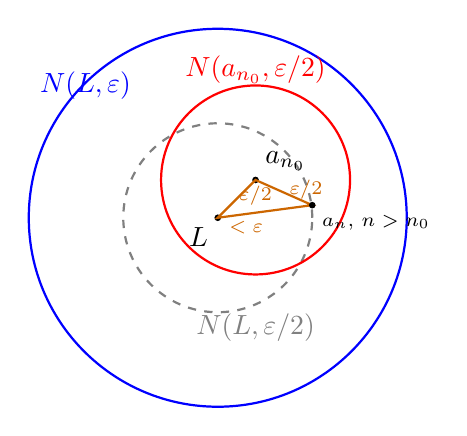
\begin{tikzpicture}[scale=.80]
            % Outer ball N(L, epsilon)
            \draw[thick, blue] (0,0) circle (3);
            \node[blue] at (-2.1,2.1) {$N(L,\varepsilon)$};

            % Inner ball N(L, epsilon/2)
            \draw[thick, dashed, gray] (0,0) circle (1.5);
            \node[gray] at (0.6,-1.75) {$N(L,\varepsilon/2)$};

            \fill (0,0) circle (1.5pt) node[below left] {$L$};

            % Point a_{n_0} inside the inner ball
            \coordinate (an0) at (0.6,0.6);

            % Ball N(a_{n_0}, epsilon/2)
            \draw[thick, red] (an0) circle (1.5);
            \node[red] at ($(an0)+(0,1.75)$) {$N(a_{n_0},\varepsilon/2)$};
            \fill (an0) circle (1.5pt) node[above right] {$a_{n_0}$};

            % Later terms a_n, n > n_0, inside N(a_{n_0}, epsilon/2)
            \coordinate (ann) at ($(an0)+(0.9,-0.4)$);
            % \fill ($(an0)+(-0.5,0.8)$) circle (1pt);
            % \fill ($(an0)+(0.3,1.0)$) circle (1pt);
            % \fill ($(an0)+(-0.9,-0.5)$) circle (1pt);

            % Triangle inequality: L -- a_{n_0} -- a_n -- L
            \draw[thick, orange!80!black] (0,0) -- (an0) -- (ann) -- cycle;
            \node[orange!80!black] at ($(0,0)!0.5!(an0) + (0.3,0.05)$) {\scriptsize $\varepsilon/2$};
            \node[orange!80!black] at ($(an0)!0.5!(ann) + (0.35,0.05)$) {\scriptsize $\varepsilon/2$};
            \node[orange!80!black] at ($(0,0)!0.5!(ann) + (-0.3,-0.25)$) {\scriptsize $<\varepsilon$};
            \fill (ann) circle (1.5pt) node[below right] {\scriptsize $a_n,\, n>n_0$};
        \end{tikzpicture}
        \end{center}
    \end{itemize}
\end{proof}

\begin{example}
    We can show divergence of Harmonic series by showing that 
    it is not Cauchy. 
    \[
        a_n = 1 + \frac{1}{2} + \hdots + \frac{1}{n}
    \]
    i.e. WTS $\exists \ep >0$,
    $\forall N > 0$,
    $\exists m > n > N$ s.t. 
    $|a_m - a_n |> \ep$.
    Take $\ep  = \frac{1}{4}$, 
    $m = 2n$,
    then 
    \begin{align*}
        a_m- a_n &= 
        \frac{1}{ n+1} + 
        \frac{1}{ n+2} + 
        \hdots
        \frac{1}{m}
        \\
        & \geq \frac{m - n}{m} \\
        & = 1 - \frac{n}{m} \\
        & = \frac{1}{2}
    \end{align*}
    Hence the harmonic series is not cauchy and therefore does not converge.
\end{example}


\begin{definition}[Monotone sequence]
    \hfill
    \begin{enumerate}
        \item $\{ a_n \} $ is \textbf{increasing} if $a_n \leq a_{n + 1}, \forall n$
        \item $\{ a_n \} $ is \textbf{decreasing} if $a_n \geq a_{n + 1}, \forall n$
    \end{enumerate}
    If $ \{ a_n \} $ is either increasing or 
    decreasing, we say it is \textbf{monotone}.
    \medskip

    Equivalently, we can define strictly increasing, strictly decreasing and
    strictly monotone.
\end{definition}

\begin{theorem}[Monotone Convergence Theorem]
    If a sequence $\{ a_n \} $ is monotone and bounded,
    then it converges. 
\end{theorem}

\begin{corollary}[Alternative statement of MCT]
    Given a monotone sequence, it is bounded if and only
    if it converges.
\end{corollary}

\begin{proof}[Proof of MCT]
    WTS that given a monotone sequence, 
    it converges if and only it is bounded.
    \medskip

    $(\implies)$: convergence implies boundedness always, 
    without requiring monotonicity.
    \medskip

    $(\impliedby)$:
    Let $\{ a_n \} $ be a monotone and bounded sequence, 
    WTS it converges. 
    \medskip

    WLOG, assume $\{ a_n \} $ increasing. 
    Since $ \{ a_n \} $ bounded, by CA, 
    $\sup \{ a_n \} $ exists, say $L$. 
    WTS $\lim_{n \to \infty}a_n = L$.
    \medskip 

    Fix $\varepsilon > 0$< by definition of supremum, 
    $\exists n_0$ s.t. $a_{n_0} > L-\varepsilon$.
    Hence 
    \begin{align*}
        & L - \varepsilon < a_n \leq L, \forall n > n_0 \\
        \implies & |a_n - L | < \varepsilon, \forall n > n_0
    \end{align*}
\end{proof}

\begin{remark}
    \hfill
    \begin{enumerate}
        \item An increasing sequence converges $\iff$ bounded from above.
        \item A decreasing sequence converges $\iff$ bounded from below.
    \end{enumerate}
\end{remark}

\begin{example}
    \textit{We can use MCT to determine the convergence
    of a sequence defined recursively,
    i.e. we prove convergence by showing
    boundedness and monotonicitiy}
    \medskip

    For example, $a_1 = 5$, $a_{n + 1} = \frac{1}{2} \left( a_n + \frac{5}{a_n} \right) $.
    We can show this is bounded by noting $a_n > 0$ and 
    therefore 
    \begin{align*}
        a_{n + 1} &= \frac{1}{2} \left( 
            \sqrt{a_n}^2 + \sqrt{ \frac{5}{a_n}}^2
        \right)  \\
        & \geq \sqrt{a_n} \sqrt{ \frac{5}{a_n}}
        = \sqrt{5}
    \end{align*}
\end{example}



\begin{proof}[Proof that interval are connected 
    \label{proof:connected-sets-in-R}]
    \medskip

    Recall theorem \ref{theorem:connected-sets-in-R}. 
    WTS that if $S \subset \mathbb{R}$ is an interval
    then $S$ is connected.
    \medskip

    Suppose $S$ disconnected. By definition, $\exists A, B$
    open and nonempty such that $S \subset A \cup B$,
    $A \cap B = \emptyset$,
    $S \cap A \neq \emptyset$,
    $S \cap B \neq \emptyset$.
    \medskip

    Let $x \in S \cap A, y \in S \cap B$. WLOG, say $x < y$.
    Let $x_1 = x, y_1 = y$. We seek sequences 
    $\{ x_n \} \subset A \cap S $,
    $\{ y_n \} \subset A \cap S $,
    such that 
    \begin{itemize}
        \item $x_n$ is increasing 
        \item $y_n$ is decreasing 
        \item $|x_n - y_n| \to 0$ as $n \to \infty$
    \end{itemize} 

    To construct such a sequence, take $z_{k + 1} = \frac{x_k + y_k}{2}$.
    \begin{itemize}
        \item if $z_{k + 1} \in A, x_{k + 1} = z_{k + 1}, y_{k + 1} = y_k$
        \item if $z_{k + 1} \in B, x_{k + 1} = x_k, y_{k + 1} = z_{k + 1}$
    \end{itemize} 
    Then 
    \[
        y_i - x_i = \frac{y_1 - x_1}{2^{i - 1}}
    \]
    Since $\{ x_n \} $ bounded and increasing, 
    $\exists a \in \mathbb{R}$ s.t. $x_n \to a$.
    Likewise
    $\exists b \in \mathbb{R}$ s.t. $y_n \to b$.
    Then
    \[
        b - a = 
        \lim_{n \to \infty} y_n - 
        \lim_{n \to \infty} x_n 
        = \lim_{n  \to \infty} (y_{n} - x_{n})
        = \lim_{n  \to \infty} 2^{-(n-1)}(y_1 = x_1)
        = 0
    \]
    Hence $b=a$.
    \medskip

    We know that $a \in (S \cap A) \setminus ( S \cap B)$ or 
    $a \in (S \cap B) \setminus (S \cap A)$. 
    Suppose $a \in S \cap A$ but $a \notin B$, by openess of $A$, 
    there is some $N(a, \varepsilon) \subset A$.
    Since $A, B$ disjoint, $N(a, \varepsilon) \subset B^c$. 
    However, $y_n \to a$, hence $\exists N>0$ s.t. $\forall n > N$,
    $y_n \in N(a, \varepsilon)$, which is a contradiction.
\end{proof}

\subsection{Subsequences}

\begin{definition}[Subsequence]
    Let $\{ a_n \}  \in \mathbb{R}$ and $\{ n_k \}_k$ be a 
    striclty increasing sequence 
    in $\mathbb{N}$, i.e. $n_k < n_{k + 1}, \forall k$, then 
    $\{ a_{n_k} \}_k$ is a subsequence of $\{ a_n \} $
\end{definition}

\begin{example}
    Take $\{ 1, -1, 1, -1, \hdots \} $, 
    \begin{itemize}
        \item $n_k = 2k - 1, \{ n_k \}_k = \{ 1, 3, 5, \hdots \}$, 
        $\{ a_{n_k} \}_k = \{ 1, 1, 1, \hdots \}  $
        \item $n_k = 2k , \{ n_k \}_k = \{ 2, 4, 6, \hdots \}$, 
        $\{ a_{n_k} \}_k = \{ -1, -1, -1, \hdots \}  $
    \end{itemize} 
\end{example}

\begin{theorem}[Subsequence of convergent sequence converges]
    If $\lim_{n \to \infty}a_n = L \in \mathbb{R}$, or $L = \pm \infty$
    then for any subsequence $\{ a_{n_k} \}_k $ of $\{ a_n \} $, 
    \[
        \lim_{k \to \infty} a_{n_k} = L
    \]
\end{theorem}

\begin{proof}
    Fix $\ep > 0$, we seek $K > 0$ s.t. $ \left| a_{n_k}  - L \right| < \ep$,
    $\forall k > K$. 
    Since $a_n$ converges, 
    \[
        \lim_{n \to \infty} a_n = L \implies \exists N > 0 \text{ s.t }
        |a_n - L | < \ep, \forall n > N
    \]
    Also, $\forall k > N, n_k \geq k \geq N$, hence $|a_{n_k} - L | < \ep$, 
    hence 
    \[
        \lim_{k \to \infty} a_{n_k = L}
    \]
\end{proof}

\begin{corollary}[Convergent subsequences whose limits disagree imply divergence]
    If $\{ a_n \} $ has two subsequences that converge to different values
    then $\{ a_n \} $ diverges and does not converge to $\pm \infty$.
\end{corollary}

\begin{theorem}[Bdd divergent sequences have at least two convergent subsequences]
    \label{theroem:bdd-dvgt-implies-multiple-cvgt-subseq}
    If $\{ a_n \} $ bounded and divergent, 
    then there exist two subsequences of $\{ a_n \} $ that converge 
    to different values. 
\end{theorem}

\begin{theorem}
    \label{theorem:bdd-implies-cvgt-subseq}
    Every bounded sequence $\{ a_n \} $ has a convergent subsequence.
\end{theorem}














%==============================================================================
% MATH 5080
% Class:        8
% Date:         Sept 17th
%==============================================================================
\begin{proof}[Proof of 
    \ref{theorem:bdd-implies-cvgt-subseq} 
    $\implies$
    \ref{theroem:bdd-dvgt-implies-multiple-cvgt-subseq}]
    \hfill

    Fix a bounded and divergent sequence $\{ a_n \}_n $
    \ref{theorem:bdd-implies-cvgt-subseq},
    $\exists \{ a_{N_k} \}_k $ and $L_1 \in \mathbb{R}$  s.t. 
    $a_{N_K} \to L$.
    By definition of divergence, we know that $ \{ a_n \} $ 
    does not converge, i.e. fix $\ep > 0$,
    \begin{align*}
        & \forall N > 0, \exists n > N \text{ s.t. } 
        |a_n - L_1| > \ep \\
        \implies & \exists \{ a_{n_l} \}_l \text{ s.t. }
        |a_{n_l} - L_1| > \ep, \forall l \in \mathbb{N}
    \end{align*}
    Since $\{ a_{n_l} \}_l $ bounded, it has a convergent subsequence by 
    \ref{theorem:bdd-implies-cvgt-subseq}. WLOG, assume $\{ a_{n_l} \} $
    converges to $L_2$. 
    \medskip

    Since $|a_{n_l} - L_2| > \ep, \forall l \in \mathbb{N}$, 
    $|L_2 - L_1| \geq \ep > 0$.
\end{proof}

\begin{proof}[Proof of \ref{theorem:bdd-implies-cvgt-subseq}]
    \hfill

    Consider 2 cases 
    \begin{itemize}
        \item Case 1: $\{ a_n \} $ finite
        Then at least one value is attained infinitely many times, 
        take a subsequence consisting only of that value, and
        we have found a convergent subsequence. 
        \item Case 2: $\{ a_n \} $ infinite
        By BW, the set of values attained by $\{ a_n \} $
        has an accumulation point say $L$.
        \medskip

        We want to construct $\{ a_[n_k] \} $ converging to $L$. 
        \begin{itemize}
            \item Let $\ep_1 \coloneq 1$, and 
            $a_{n_1} \in N^*(L, \ep_1) \cap \{ a_n \}$.
            \item Let $\ep_2 = \frac{1}{2}$. 
            Since $N^*(L, \ep_2) \cap \{ a_n \}_{n \geq n_1 + 1} $ has infinitely
            many points, $\exists n_2 > n$ s.t. $a_{n_2} \in N^*(L, \ep_2)$. 
            \item Repeat this process, if $a_{n_1}, a_{n_2}, \hdots a_{n_k}$ chosen, 
            let $\ep_{k + 1} = \frac{1}{k + 1}$ and pick
            \[
                a_{n_{k + 1}} \in N^*(L, \ep_{k + 1}) \cap \{ a_n \}_{n \geq n_K + 1}
            \], 
            and we have constructed a subsequence $\{ a_{n_k} \} $ such that 
            $a_{n_k} \rightarrow L$
        \end{itemize} 
    \end{itemize} 
\end{proof}

\begin{definition}[Subsequential limits]
    Let $\{ a_n \} \subset \mathbb{R}$, the set of subsequential limits of 
    $\{ a_n \} $ is the set of $x \in \mathbb{R} \cup \{ \pm \infty \} $ such that 
    some subsequence $\{ a_{n_k} \} $ converges to $x$.
\end{definition}

\begin{remark}
    $\{ a_n \} $ bounded if and only if its set of subsequential limits 
    is a nonempty and bounded subset of $\mathbb{R}$.
\end{remark}

\begin{definition}[Extended reals]
    In the extended real number system $R \cup \{ \pm \infty \} $,
    \begin{itemize}
        \item we have order
            \[
                -\infty < x < \infty, \forall x
            \]
        \item we do not have a field 
        \item we have the following conventions, $\forall x \in \mathbb{R}$
        \begin{align*}
            & x + \infty = \infty \\
            & x - \infty =  - \infty \\
            & \frac{x}{+ \infty} = \frac{x}{- \infty} = 0 \\
            &x > 0 \implies x \times (\pm \infty) = \pm \infty \\
            &x < 0 \implies x \times (\pm \infty) = \mp \infty \\
            \end{align*}
    \end{itemize} 
\end{definition}


\begin{definition}[Limit superior, limit inferior]
    The limit superior of $\{ a_n \} $ is defined as the supremum 
    of the set of subsequential limit, denoted as 
    \[
        \limsup_{ n \to \infty} a_n \in \mathbb{R} \cup \{ \pm \infty \} 
    \]

    Similarly, the limit inferior is defined as the 
    infimum of the set of subsequential limits, denoted
    $\liminf_{n \to \infty} a_n$.
\end{definition}

\begin{remark}
    The limit inferiors and superiors always exists for any sequence 
    in $\mathbb{R} \cup \{ \pm \infty \} $.
    \begin{itemize}
        \item $\{ a_n \} $ bounded from above $\iff$ 
        $\limsup_{n \to \infty} a_n \in \mathbb{R} \cup \{ -\infty \} $. 
        Otherwise $\limsup_{n \to \infty} a_n = \infty$. 
        \item $\{ a_n \} $ bounded from bleow $\iff$ 
        $\liminf_{n \to \infty} a_n \in \mathbb{R} \cup \{ \infty \} $. 
        Otherwise $\liminf{n \to \infty} a_n = -\infty$. 
        \item $\{ a_n \} $ bounded $\implies$
        $\liminf a_n, \limsup a_n \in \mathbb{R}$.
    \end{itemize} 
\end{remark}


\begin{proposition}
    \hfill
    \begin{enumerate}
        \item $\liminf_{n \to \infty} a_n \leq \limsup_{n \to \infty}a_n$
        \item A sequence converges if and only if its limsup and liminf agree
        \[
            \lim_{n \to \infty} a_n = L \in \mathbb{R} \cup \{ \pm \infty \} 
            \iff 
            \liminf_{n \to \infty} a_n = 
            \limsup_{n \to \infty} a_n = 
            L
        \]
    \end{enumerate}
\end{proposition}
\begin{proof}
    \textbf{
        WTS
        $\lim_{n \to \infty} a_n = L$
        $\implies$
        $\liminf_{n \to \infty} a_n = \limsup_{n \to \infty} a_n = L$
    }
    Since every subsequence of a convergent sequence converges to the 
    same limit.
    \medskip

    \textbf{
        WTS
        $\liminf_{n \to \infty} a_n = \limsup_{n \to \infty} a_n = L$
        $\implies$
        $\lim_{n \to \infty} a_n = L$
    }
    ATC otherwise, i.e. 
    \begin{align*}
        & \lim_{n \to \infty} a_{n} \neq L 
        \implies & \exists \{ a_{n_k} \} \text{ s.t. }
        \exists \ep_0, |a_{n_k} - L | > \ep_0, \forall k \in \mathbb{N}
    \end{align*}
    Since $\liminf a_n = \limsup a_n = L$, $\{ a_n \} $ 
    must be bounded. Hence $ \{ a_{n_k} \} $ also bounded.
    Hence $\{ a_{n_k} \} $ has a convergent subsequence,
    which we still denote $\{ a_{n_k} \} $. 
    Since this is also a subsequence of the original $\{ a_n \} $, we know 
    that $\lim_{k \to \infty}a_{n_k} = L$. However, this leads
    to a contradiction because take $\ep = \frac{\ep_0}{2}$, then
    $\forall k, |a_{n_k} - L | > \ep_0 > \ep$.
\end{proof}


\begin{proposition}
    If $\{ a_n \} $ is bounded then its set of subsequential limits is closed. 
\end{proposition}

\begin{proof}
    \textit{
        The idea is to take any accumulation point
        in the set of subsequential limits of $a_n$,
        and show that some subsequence indeed
        converges to that accumulation point.
    }
    \medskip

    If $\{ a_n \} $ bounded, 
    then all of its subsequential limits are in $\mathbb{R}$.
    Let $E$ denote the set of subsequential limits. 
    WTS that $E$ contains all of its accumulation points, 
    i.e. $\forall p \in E^{\prime}, p \in E$. 
    \medskip

    Now we want to construct a subsequence that 
    converges to $p$
    \begin{itemize}
        \item First choose $p_1 \in N^*(p, 1) \cap E$. 
    Let $\ep_1 = 1 - |p-p_1| > 0$.
    $\exists a_{n_1}$ s.t. $|a_{n_1} - p_1| < \ep_1 \implies$
    $|a_{n_1} - p| < 1$.
        \item $\vdots$
        \item 
    Suppose $a_{n_1} , \hdots a_{n_{k - 1}}$ are found, s.t. 
    $n_1 < n_2 < \hdots n_{k-1}$,
    choose $p_k \in N^*(p, \frac{1}{k}) \cap E$. 
    Let $\ep_k = \frac{1}{k} - |p - p_k| > 0$.
    $\exists a_{n_k}$ s.t. $n_k > n_{k-1}$ and 
    $|a_{n_k} - p_k| < \ep_k$. 
    Hence $|a_{k_k} - p| < \frac{1}{k}$. 
    \end{itemize} 

    Therefore $a_{n_k} \to p$ and $p \in E$.
\end{proof}



\begin{theorem}
    \label{theorem:limsup-properties}
    If $\{ a_n \} $ is bounded and $x \in \mathbb{R}$, TFAE 
    \begin{enumerate}
        \item $\limsup_{n \to \infty} a_n = x$ 
        \item 
        \begin{enumerate}
            \item $\forall \ep > 0, \exists N > 0$ s.t. 
            $\forall n > N$, $a_n < x + \ep$ AND
            \item $\forall \ep > 0, \forall N > 0$,
            $\exists n > N$, s.t. $a_n > x - \ep$
        \end{enumerate}
        \item \begin{enumerate}
            \item There is $\{ a_{n_k} \} $ that converges to $x$ 
            AND
            \item If $\{ a_{n_j} \} $ converges, then 
            $\lim_{j \to \infty} a_j \leq x$
        \end{enumerate}
        \item Let $b_n = \sup_{m \geq n} a_m$, then $b_n$ converges
        and $\lim_{n \to \infty} b_n = x$
    \end{enumerate}
\end{theorem}

% \begin{proof}[Proof of 
%         \ref{theorem:limsup-properties},
%         1 $\iff$ 2
%     ]
%     \begin{itemize}
%         \item 1 $\implies$ 2(a). 
%         \medskip

%         ATC otherwise, fix $\ep > 0$, suppose 
%         $\not \exists N > 0$ s.t. $\forall n > N$, $a_n < x + \ep$.  Then $\exists \{ a_{n_k} \}_k $ s.t. $a_{n_k} \geq x + \ep, \forall k$. 
%         By \ref{theorem:bdd-implies-cvgt-subseq}, it has a subsequence 
%         that converges to some $L \geq x + \ep$, hence a contradiction. 
%         \item 1 $\implies$ 2(b)
%         \medskip

%         ATC otherwise, then $\exists N > 0$ s.t. $\forall n > N$, 
%         $a_n \leq x - \ep$. Hence all convergent subsequences have limits $x < \ep$< 
%         \medskip 

%         Hence $x \leq x - \ep$, which leads to a contradiction.
%         \item 2 $\implies$ 1.
%         \medskip

%         Fix $\ep > 0$, by \ref{theorem:limsup-properties},
%         2.(a), all subsequential limits are upper bound by 
%         $x + \ep$.
%         \[
%             \limsup a_n \leq x + \ep \implies \limsup a_n \leq x + \ep
%         \]
%         We claim that $\limsup a_n = x$. If not, then $\limsup (a_n) < x$< 
%         le $\ep = \frac{1}{2}(x - \limsup(a_n)) > 0$. By 
%         2.(b), we can find a subsequence $\{ a_{n_k} \} $ s.t. 
%         $a_{n_k} > x - \ep$. By
%         \ref{theroem:bdd-dvgt-implies-multiple-cvgt-subseq},
%         WLOG, assume $a_{n_k} \to L$, then 
%         \[
%             L \geq x - \ep > \limsup a_N
%         \]
%         which is a contradiction.
%     \end{itemize}
% \end{proof}

% \remind{fill in additional material from class 8}

\begin{proof}[Proof of 
        \ref{theorem:limsup-properties},
    ]
    In general, let $E$ denote the 
    set of subsequential limits of $a_n$.
    \begin{itemize}
        \item (1) $\iff$ (2)
        \begin{enumerate}
            \item (1) $\implies$ (2)
            \begin{itemize}
                \item (1) $\implies$ (2a): ATC otherwise,
                then $\exists$ infinitely many terms
                where $a_n \geq x + \ep$.
                Then they form a subsequence $ \{ a_{n_k} \} $
                which is also bounded. 
                Hence this subsequence itself has a convergent
                subsequence converging to some
                limit $L \geq x + \ep > x$. 
                Hence contradicting the assumption
                that $x$ is a supremum.
                \item (1) $\implies$ (2b)
                ATC otherwise, then only finitely many terms
                $a_n > x - \ep$. Hence,
                $\exists N >0$ s.t. $\forall n > N$,
                $a_n \leq x - \ep$. Hence 
                all subsequential limits must be less 
                than $x - \ep$. This contradicts
                the assumption that $x$ is a minimal upper bound.
            \end{itemize} 
            \item (1) $\impliedby$ (2): Fix any $\ep > 0$, 
            $\exists N \text{ s.t. } \forall n > N$,
            $a_n < x + \ep$.
            Hence any subsequential limit is smaller than $x + \ep$.
            Therefore $\limsup a_n \leq x + \ep$. Since
            $\ep$ is arbitrary, $\limsup a_n \leq x$.
        \end{enumerate}
        \item (1) $\iff$ (3)
        \begin{enumerate}
            \item (1) $\implies$ (3)
            Since the set of subsequential limits is closed,
            the supremum is in $E$. Hence
            some subsequence converges to it. 
            By definition of supremum, $x \geq p, \forall p \in E$.
            \item (1) $\impliedby$ (3): by definition
        \end{enumerate} 
        \item (1) $\iff$ (4)
        \begin{enumerate}
            \item (1) $\implies$ (4): 
            Since $\{ a_n \} $ bounded, 
            $\{ \sup_{m \geq n} a_m\}_n $ is also bounded
            by the same bounds. 
            Also note
            \begin{align*}
                \sup_{m \geq n + 1} a_m \leq
                \sup_{m \geq n} a_m
            \end{align*}
            Hence the sequence is decreasing. 
            By MCT
            \begin{align*}
                \lim_{n \to \infty}
                \sup_{m \geq n} a_m = L \in \mathbb{R}
            \end{align*}
            It suffices to show that $L = x$. 
            Fix $\ep > 0$. 
            \begin{itemize}
                \item By (2a): $\exists N > 0$ s.t. $\forall n > N$
                $a_n < x + \frac{\ep}{2}$. Hence 
                \[
                    b_n = \sup_{m \geq n} a_m \leq 
                    x + \frac{\ep}{2} 
                    < x + \ep
                \]
                Hence $L = \lim_{n \to \infty}b_n \leq x + \ep$
                $\implies$
                $L \leq x$
                \item By (2b): $\forall n > 0$, 
                \begin{align*}
                    b_n = \sup_{m \geq n} a_m > x  - \ep
                \end{align*}
                Hence $L = \lim_{n \to  \infty}b_n \geq x - \ep$
                $\implies$
                $L \geq x$.
            \end{itemize} 
            \item (1) $\impliedby$ (4):
            Prove by showing (4) $\implies$ (3).
            \medskip

            We pick 
            \begin{itemize}
                \item $n_1$ s.t. $a_{n_1} \geq \sup_{m \geq 1} a_m - 1$
                \item $n_2$ s.t. $n_2 > n_1$ and 
                $a_{n_2} \geq \sup_{m \geq n_1 + 1} a_m - \frac{1}{2}$.
                \item $\vdots$
                \item $n_k$ s.t. $n_k > n_{k-1}$ s.t. $a_{n_k} \geq$
                $\sup_{m \geq n_{k-1} + 1} a_m - \frac{1}{k}$.
            \end{itemize} 
            Let $L = \lim_{n \to \infty} \sup_{m \geq n} a_m$.
            \medskip

            WTS $\lim_{n \to \infty}a_{n_k} = L$.
            Fix $ \ep > 0$. Choose $N > 0$ s.t. 
            $\forall n > N$,
            \[
                \left| \sup_{m \geq n} a_m - L\right|  < \frac{\ep}{2}
            \]
            Then take $N_0 = \max \{ N + 1, \frac{2}{\ep} \} $,
            one has $\forall k > N_0$, 
            \begin{align*}
                \left|a_{n_k}- L \right| &\leq 
                \left| a_{n_k} - \sup_{m \geq n_{k -1} + 1} a_m \right|  
                +
                \left| \sup_{m \geq n_{k -1} + 1} - L\right|  \\
                & \leq \frac{1}{k} + \frac{\ep}{2} \\
                & \leq \frac{\ep}{2} + \frac{\ep}{2} = \ep
            \end{align*}
            Hence we have shown (3a). 
            \medskip

            Let $\{ a_{n_k} \} $ be any convergent subsequence.
            of $ \{ a_n \} $. We have
            \begin{align*}
                &a_{n_k} \leq \sup_{m \geq n_k} a_m, \forall k \\
                \implies & 
                \lim_{k \to \infty} a_{n_k} \leq 
                \lim_{k \to \infty} \sup_{m \geq n_k} a_m = L
            \end{align*}
        \end{enumerate}
    \end{itemize}
\end{proof}






%==============================================================================
% MATH 5080
% Class:        9
% Date:         Sept 22nd
%==============================================================================

\newpage

\section{Limits and Continuity of Functions}

\subsection{Limits of Functions}

\begin{definition}[Limits of functions]
    Let $f: D \to \mathbb{R}, D \subset \mathbb{R}$,  and $c$
    be an accumulation point of $D$. We say $L \in \mathbb{R}$
    is the limit of $f$ at $c$ if $\forall \ep > 0, \exists \delta > 0$
    s.t. $|f(x) - L | < \ep$ whenever $0 < |x - c| < \delta$ and 
    $x \in D$,
    denoted 
    \[
        \lim_{x \to c} f(x) = L
    \]
    
\end{definition}

\begin{remark}
    \hfill
    \begin{enumerate}
        \item We define limits of functions only on accumulation points
        in the domain. 
        \item Note that $0 < |x - c|$, i.e. we care about $x \in N^*(c, \delta)$.
        We do not need $f(c)$ to be defined. 
        When it is defined, $\lim_{x \to c}f(x)$ has nothing to do with
        $f(c)$.
        \item The limit of a function at $c$ is unique.
    \end{enumerate}
\end{remark}

\begin{example}
    Show $\lim_{x \to 2}x^2 = 4$.
    \remind{Add in later}.
\end{example}


\begin{theorem}[Equivalence between limit of function and limit of a sequence]
    \hfill

    Let $f: D \to \mathbb{R}, c \in D^{\prime}$, TFAE
    \begin{enumerate}
        \item $\lim_{x \to c}f(x)= L$
        \item For every $ \{ a_n \} \subset D$ s.t. $a_n \to c$ but 
        $a_n \neq c, \forall n$, we have 
    \[
        \lim_{n \to \infty} f(a_n) = L
    \]
    \end{enumerate}
\end{theorem}

\begin{remark}
    \hfill
    \begin{itemize}
        \item 
    This result allows us to work with limits of sequences whenever
    we want to talk about limits of continuous functions
        \item We can make the above theorem weaker by only requiring $a_n \neq c$
        $\forall n > N$ for some $N$.
    \end{itemize} 
\end{remark}

\begin{example}
    $\lim_{x \to \infty} \sin \left( \frac{1}{x} \right) $ does not 
    have a limit.
\end{example}

\begin{proof}
    To show (1) $\implies$ (2): 
    \medskip
    Assume $\lim_{x \to c}f(x) = L$, 
    Fix $\{ a_n \} \subset D$ s.t. $a_n \to c, a_n \neq c, \forall n \in \mathbb{N}$
    WTS $\lim_{n \to \infty}f(a_n) = L$. 
    \medskip

    By definition, $\lim_{x \to c}f(x) = L \implies \exists \delta$ s.t. 
    $0 < |x-c| < \delta \implies |f(x) - L | < \ep$.
    Since $a_n \to c \iff \lim_{n \to \infty} a_n = c$ and $a_n \neq c, \forall n$,
    $\exists N > 0$ s.t. $\forall n > N$
    \begin{align*}
        0 < |a_n - c | < \delta \implies |f(a_n) - L | < \delta
    \end{align*}
    \medskip

    To show (2) $\implies$ (1): Assume $f(x)$ does not converge to $L$
    as $x \to c$, 
    $\exists \ep > 0$ s.t. $\forall \delta > 0$, 
    $\exists x \in N^*(c, \delta) \cap D$ s.t. $|f(x) - L | \geq \ep$.
    \begin{itemize}
        \item Let $\delta_1 = 1, a_1 \in N^*(c, \delta_1) \cap D$ s.t. $|f(a_1) - L | \geq \ep$
        \item Let $\delta_2 = \frac{1}{2}, a_2 \in N^*(c, \delta_2) \cap D$ s.t. $|f(a_2) - L | \geq \ep$
        \item $\vdots$
        \item $\delta_n = \frac{1}{n}, a_n \in N^*(c, \delta_n) \cap D$ s.t. $|f(a_n) - L | \geq \ep$
    \end{itemize} 
    Since $a_n$ satisfies $a_n \to c, a_n \neq c$, by assumption, 
    $\lim_{n \to \infty} f(a_n) = L$. This contradicts $|f(a_n) - L | \geq \ep$.
\end{proof}

\begin{corollary}
    Let $f: D \to \mathbb{R}, c \in D^{\prime}$, TFAE
    \begin{enumerate}
        \item $f$ doesn't have a limit at $c$
        \item There exists a sequence $\{ a_n \}  \subset D$
        that converges to $c$ with $a_n \neq c, \forall n$ s.t. 
        $\{ f(a_n) \} $ diverges.
    \end{enumerate} 
\end{corollary}

\begin{remark}
This is very useful for proving that a limit DNE.
\end{remark}

\begin{proposition}[Algebraic operations of limits of functions]
    Let $f: D \to \mathbb{R}, c \in D^{\prime}$. 
    Suppose $\lim_{x \to c}f(x) = L$,
    $\lim_{x \to c}g(x) = M$. 
    Then 
    \begin{enumerate}
        \item $\lim_{x \to c}(f+ g) (x) = L + M$.
        \item $\lim_{x \to c}(f\cdot g) (x) = LM$.
        \item $\lim_{x \to c}kf(x) = kL, \forall k \in \mathbb{R}$.
        \item If $g(x) \neq 0, \forall x \in D$, and $M \neq 0$, then 
        \[
            \lim_{x \to c} \frac{f}{g}(x) = \frac{L}{M}
        \]
    \end{enumerate} 
\end{proposition}

\begin{definition}[One sided limits]
    \hfill
    \begin{enumerate}
        \item We say that $\lim_{x \to c^-}f(x) = L$ if 
        $\forall \ep > 0$, $\exists \delta > 0$ s.t. 
        $c - \delta < x < c \implies |f(x) - L | < \ep$ 
        \item We say that $\lim_{x \to c^+}f(x) = L$ if 
        $\forall \ep > 0$, $\exists \delta > 0$ s.t. 
        $c < x < c  + \delta\implies |f(x) - L | < \ep$ 
    \end{enumerate} 
\end{definition}

\begin{proposition}[
        Equivalence of one-sided and two-sided limits
    ]
    \begin{align*}
        \lim_{x \to c}f(x) = L
        \iff
        \lim_{x \to c^-}f(x) =
        \lim_{x \to c^+}f(x) =
        L
    \end{align*}
\end{proposition}

\subsection{Continuous functions}


\begin{definition}[Continuity]
    Let $f: D \to \mathbb{R}$
    \begin{enumerate}
        \item (\textbf{Continuity at a point})
    Let $c \in D$,  
    we say $f$  is \textbf{continuous at $c$} if 
    $\forall \ep > 0, \exists \delta > 0$ s.t. 
    $|f(x) - f(c)| < \ep$ whenever 
    $|x - c| < \delta$.
        \item (\textbf{Continutiy over a set}): Let $S \subset D$
    if $\forall c \in S$, $f$ is continuous at $c$, then we say 
    that $f$ is \textbf{contiuous on $S$}.
        \item (\textbf{Continuous function}): if $f$ is continuous
    on $D$, then we say $f$ is a \textbf{continuous function}.
    \end{enumerate} 
\end{definition}

\begin{remark}
    \hfill
    \begin{enumerate}
        \item Compared to the definition of 
        the limit of a function at a point,
        we now require $c \in D$ instead of $c \in D^{\prime}$.
        \item We now allow $x = c$.
        \item We cannot immediately apply the previous definition 
        of limit of a function at point to define continuity
        because 
        we don't know that $c$ is an accumulation point.
        \item Depending on whether $c$ is an accumulation point
        or an isolated point, we have different conditions
        that are required for the continuity of $f$ at $c$. 
        Refer to the following two propositions.
        % \item If $c$ is an isolated pint of the domain, then any function is 
        % continuous at $c$.
        % \item If $c$ is an accumulation point, $f$ continuous at $c$ $\iff$
        % $\lim_{x \to c}f(x) = f(c)$.
    \end{enumerate} 
\end{remark}

\begin{proposition}[Any function is continuous at isolated point]
    If $c$ is an isolated point of $D$, then 
    $f$ is always continuous at $c$.
\end{proposition}

\begin{proof}
    $c$ isolated $\implies \exists \delta_0$ s.t.
    $N^*(c, \delta_0) \cap D = \emptyset$. 
    Fix any $\ep > 0$, pick $\delta = \delta_0$. 
    Then, 
    \begin{align*}
        x \in N(c, \delta) \implies x = c \implies
        |f(x) - f(c) | = 0 < \ep
    \end{align*}
\end{proof}


\begin{proposition}
    If $c$ is an accumulation point of $D$, then 
    $f$ is continuous at $c$ if and only if $\lim_{x \to c}f(x)=$
    $f(c)$.
\end{proposition}

\begin{proof}
    By definition, \remind{exercise}.
\end{proof}




\begin{proposition}[Equivalent characterization of continuity]
    $f$ is continuous at $c$ if any only if for any neighborhood 
    of $f(c)$, say $V = N(f(c), \ep), \forall \ep$, 
    there exists a neighborhood $U = N(c, \delta)$ such that 
    $f(U \cap D) = V$.
\end{proposition}

\begin{theorem}
    Let $f: D \to \mathbb{R}, c \in D$ , TFAE
    \begin{enumerate}
        \item $f$ is continuous at $c$
        \item If $\{ a_n \} \subset D $ s.t. $a_n \to c$, then 
        \[
            \lim_{n \to \infty} f(a_n) = f(c)
        \]
    \end{enumerate} 
\end{theorem}

\begin{proof}
    \remind{revisit this proof}
    \medskip

    $c$ is either an isolated point or an accumulation point. 
    \begin{enumerate}
        \item Case 1: $c$ isolated.
        We want to show that (1) and (2) are always true. 
        \begin{itemize}
            \item We already know that (1) is always true, 
            any $f$ is continuous at $c$ if $c$ isolated.
            \item WTS (2). Fix any $\{ a_n \}$ converging to $c$. 
            Since $c$ isolated, $\exists \ep > 0$ s.t. 
            $N^*(c, \ep) \cap D = \emptyset$. 
            Since $a_n \to c, \exists N$ s.t. $\forall n > N$,
            $|a_n - c | < \ep \implies a_n = c \implies f(a_n) = f(c)$.
        \end{itemize} 
        \item Case 2: $c$ accumulation point
            \begin{itemize}
                \item (1) $\implies$ (2): 
                \begin{align*}
                    f \text{continuous at } c 
                    & \implies \lim_{x \to c}f(x) = f(c) \text{ by definition} \\
                    & \implies \{ a_n \} \subset D, a_n \neq c, a_n \to c \implies 
                    \lim_{n \to \infty} f(a_n) = f(c)
                \end{align*}
                ATC otherwise, i.e. $\{ a_n \} \subset D, a_n \to c, \lim_{n \to \infty}f(a_n) \neq f(c)$
                then $\exists \ep > 0$ and some subsequence $\{ a_{n_k} \} $
                such that $a_{n_k} \to c$ but $ \left| f(a_{n_k}) - f(c)\right|  > \ep$.
                Hence $a_{n_k} \neq c, \forall k$. However, this contradicts with
                the result.
                \item (2) $\implies$ (1): 
                Assume (2), then we immediately have 
                \begin{align*}
                    &\{ a_n \} \subset D, a_n \neq c, a_n \to c \implies 
                    \lim_{n \to \infty} f(a_n) = f(c) \\
                    & \implies \lim_{x \to c}f(x) = f(c) \\
                    & \implies f \text{ continuous at } c
                \end{align*}
            \end{itemize} 
    \end{enumerate} 
\end{proof}

\begin{theorem}
    $f, g: D \to \mathbb{R}, c \in D$. Suppose $f, g$ both
    continuous at $c$. Then the following functions are also
    continuous at $c$:
    \begin{enumerate}
        \item $f + g$
        \item $fg$
        \item $kf$
        \item $ \frac{f}{g}$, if $g(c) \neq 0$
    \end{enumerate} 
\end{theorem}

\begin{remark}
    The assumption that $\exists \ep > 0$
    s.t. 
    $\forall x \in N(c, \ep), g(x) \neq 0$
    is necessary and sufficient condition for $g(c) \neq 0$.
\end{remark}

\begin{proof}
    We prove using the previous theorem, and the 
    analogous result for limits.
\end{proof}


\begin{theorem}
    Let $f: D \to \mathbb{R}, g: E \to \mathbb{R}$ s.t.
    $f(D) \subset E$, 
    suppose $f$ continuous at $c \in D$, $g$ continuous at $f(c) \in E$, 
    then $g \circ f : D \to \mathbb{R}$ is continuous at $c$.
\end{theorem}

\begin{proof}
    Fix a neighborhood $V$ of $g \circ f(c)$, we seek a neighborhood $U$
    such that $g \circ f( U \cap D) \subset V$. 
    \medskip

    Since $g$ continuous at $f(c)$, $\exists $ a neighborhood $W$
    of $f(c)$ such that $g(W \cap E) \subset V$. 
    \medskip

    Since $f$ continuous at $c$, $\exists$ a neoighboord $U$ of $c$ such that 
    $f(U \cap D) \subset W$.
\end{proof}

\begin{remark}
    $f(D) \subset E \implies f(U \cap D) \subset W \cap E$
    $\implies g \circ f(U \cap D) \subset g(W \cap E) \subset V$.
    \begin{center}
    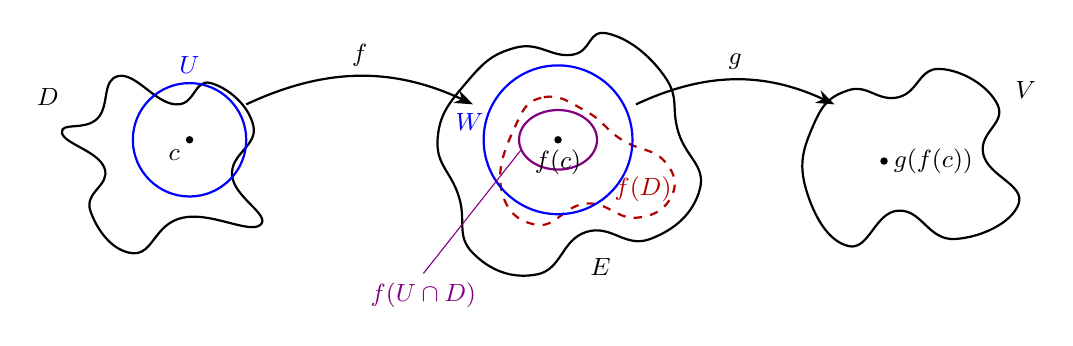
\begin{tikzpicture}[scale=0.9, every node/.style={font=\small}]
        % domain D and neighborhood U of c
        \draw[thick] plot[smooth cycle, tension=0.8]
            coordinates {(-1.5,0.4) (-1.0,0.6) (-0.7,1.2) (0.1,0.8) (0.6,1.1) (1.2,0.5) (0.9,-0.2) (1.3,-0.9) (0.2,-0.8) (-0.5,-1.3) (-1.1,-0.7) (-0.9,-0.1)};
        \draw[thick, blue] (0.3,0.3) circle (0.8);
        \fill (0.3,0.3) circle (1.5pt) node[below left] {$c$};
        \node at (-1.7,0.9) {$D$};
        \node[blue] at (0.3,1.35) {$U$};

        % E containing f(D), and neighborhood W of f(c)
        \begin{scope}[xshift=5.5cm]
            \draw[thick] plot[smooth cycle, tension=0.8]
                coordinates {(-1.7,0.3) (-1.3,1.1) (-0.6,1.6) (0.2,1.5) (0.7,1.8) (1.5,1.2) (1.7,0.4) (2.0,-0.4) (1.3,-1.1) (0.4,-1.0) (-0.3,-1.6) (-1.2,-1.3) (-1.4,-0.5)};
            \draw[thick, dashed, red!70!black] plot[smooth cycle, tension=0.8]
                coordinates {(-0.6,0.5) (-0.2,0.9) (0.4,0.7) (0.9,0.3) (1.5,0.0) (1.6,-0.5) (1.1,-0.8) (0.4,-0.6) (-0.3,-0.9) (-0.8,-0.4)};
            \draw[thick, blue] (0,0.3) circle (1.05);
            \draw[thick, violet] (0,0.3) ellipse (0.55 and 0.42);
            \fill (0,0.3) circle (1.5pt) node[below] {$f(c)$};
            \node[violet] (fUD) at (-1.9,-1.9) {$f(U \cap D)$};
            \draw[violet, thin] (fUD.north) -- (-0.52,0.16);
            \node[red!70!black] at (1.2,-0.4) {$f(D)$};
            \node[blue] at (-1.25,0.55) {$W$};
            \node at (0.6,-1.5) {$E$};
        \end{scope}

        % V around g(f(c))
        \begin{scope}[xshift=10.5cm]
            \draw[thick] plot[smooth cycle, tension=0.8]
                coordinates {(-1.4,0.5) (-0.9,1.0) (-0.2,0.9) (0.4,1.3) (1.2,0.8) (1.0,0.1) (1.5,-0.6) (0.6,-1.1) (-0.2,-0.7) (-0.9,-1.2) (-1.5,-0.4)};
            \fill (-0.4,0) circle (1.5pt) node[right] {$g(f(c))$};
            \node at (1.6,1.0) {$V$};
        \end{scope}

        % maps
        \draw[-{Stealth}, thick] (1.1,0.8) to[bend left=25] node[above] {$f$} (4.3,0.8);
        \draw[-{Stealth}, thick] (6.6,0.8) to[bend left=25] node[above] {$g$} (9.4,0.8);
    \end{tikzpicture}
    \end{center}
\end{remark}

\begin{theorem}[Limit passes through continuous functions]
    \hfill

    Let $f: D \to \mathbb{R}, g: E \to \mathbb{R}$,
    $f(D) \subset E$, 
    suppose $\lim_{x \to c}f(x) = L \subset E$ and 
    $g$ is continuous at $L$,
    then 
    \[
        \lim_{x \to c} g(f(x)) = 
        g \left( \lim_{x \to c} f(x)\right)  = 
        g(L)
    \]
\end{theorem}

\begin{example}
    If however, we only have 
    $\lim_{x \to c} f(x) = L$,
    $\lim_{y \to L} g(y) = M$,
    then in general we \textbf{do not have}
    $\lim_{x \to c} g(f(x)) = M$.
    \medskip

    For example, take $f(x) = L$  a constant function, 
    then $\lim_{x \to c}g(f(x))= g(L)$,
    which is not necessarily equal to 
    $\lim_{y \to L}g(y)$, unless we know
    that $g$ is continous at $L$.
\end{example}

\begin{proof}
    Fix $\ep >0$. WTS $\exists \delta > 0$ s.t. 
    if 
    $0 < |x - c | < \delta $ and $x \in D$, 
    then $|g(f(x)) - g(L) | < \ep$. 
    \medskip

    By definition of continituity of $g$ at $L$,
    for $\ep$, $\exists \eta > 0$ s.t. 
    $|y - L | < \eta, y \in E \implies $
    $|g(y) - g(L) | < \ep$
    \medskip

    By definition of limit of $f$ at $c$,
    since $\lim_{x \to c}f(x) = L$,
    $\exists \delta > 0$ s.t. 
    $0 < | x - c | < \delta, x \in D$, 
    $\implies |f(x) - L | < \eta$.
    \medskip

    Since $f(D) \subset E$, 
    $0 < | x - c | < \delta, x \in D$
    $\implies |f(x) - L | < \eta, f(x) \in E$
    $\implies |g(f(x)) - g(L) | < \ep$.
\end{proof}

\begin{example}
    $f(x) = x^2, D = (-1, 1), f(D) = [0, 1)$
\end{example}

\begin{remark}
    Continuous functions do not necessarily preserve
    openess.
\end{remark}

\begin{theorem}[
    Preimage of open set in $\mathbb{R}$
    is open
]
Let $f$ be a function on $\mathbb{R}$, TFAE
\begin{itemize}
    \item $f$ is continuous on $\mathbb{R}$.
    \item For any open $V \subset \mathbb{R}, f^{-1}(V)$ is open.
\end{itemize} 
\end{theorem}

\begin{remark}
    This can be made stronger into the following theorem.
\end{remark}

\begin{theorem}[Preimage of open is open]
    Let $f: D \to \mathbb{R}$, TFAE 
    \begin{enumerate}
        \item $f$ is continuous on $D$
        \item Any open image has a preimage that is the 
        intersection of an open set and the domain.
        \[
        \forall V \subset \mathbb{R}, 
        V \text{ open},
        \exists U \subset \mathbb{R} 
        \text{ s.t. }
        f(U \cap D) = V, 
        \text{ i.e. }
        f^{-1} = U \cap D.
        \]
    \end{enumerate} 
\end{theorem}

\begin{remark}
    We want to say that any open image has an 
    open pre-image, but that is not always true.
    We can only say $f^{-1}(V) = U \cap D$
    for some open $U$.
\end{remark}

\begin{corollary}
    Let $f: D \to \mathbb{R}$ , TFAE
    \begin{enumerate}
        \item $f$ is continuous on $D$
        \item for any closed $V \subset \mathbb{R}$,
        $\exists U \subset \mathbb{R}$, $U$ closed, 
        s.t. 
        $f^{-1}(V) = D \cap U$.
    \end{enumerate} 
\end{corollary}

\begin{proof}
    We prove a special case where $D = \mathbb{R}$.
    \medskip

    (1) $\implies$ (2): Assume $f$ continous on $D$, let $V$ be open. WTS $f^{-1}(V)$
    open. 
    \medskip

    Fix any $c \in f^{-1}(V)$. WTS $\exists \ep > 0$  s.t $N(c, \ep) \subset f^{-1}(V)$.
    \medskip

    Since $c \in f^{-1}(V), f(c) \in V$. Since $V$ open, $\exists$ a neighborhood
    of $f(c)$ say $U$ s.t. $U \subset V$.
    \medskip
    
    Since $f$ continuous at $c$, by definition, $\exists \ep > 0$  s.t. 
    $f(N(c, \ep)) \subset U \subset V$. Hence $N(c, \ep) \subset f^{-1}(V)$.
    \medskip

    (2) $\implies$ (1): WTS $f$ continuous at any $c \in \mathbb{R}$. Let $V$ 
    be any neighborhood of $f(c)$. WTS $\exists$ a neighborhood of $c$, say $U$ s.t.
    $f(U) \subset V$. 
    By assumption, we know $f^{-1}(V)$ is open. Since $c \in f^{-1}(V)$, 
    $c$ must be an interior point of $f^{-1}(V)$. So there exists a neighborhood 
    of $c$ say $U$ s.t. $U\subset f^{-1}(V)$, i.e. $f(U) \subset V$.
\end{proof}














%==============================================================================
% MATH 5080
% Class:        10
% Date:         Sept 29th
% cross checked against lecture notes
%==============================================================================

\subsection{Properties of continuous functions: compactness}

\begin{remark}
    Continuity does not preserve closedness.
\end{remark}
\begin{example}
    Consider $D = [1, \infty), f(x) = \frac{1}{x}$. Then the domain is closed,
    but the image $f(D) = (0, 1]$ and is not closed.
\end{example}
\begin{remark}
    Continuity does not preserve boundedness.
\end{remark}
\begin{example}
    Consider $D = [0, 1], f(x) = \frac{1}{x}$. 
    Then the domain is bounded,
    but the image $f(D) = [1, \infty)$ and is not bounded.
\end{example}

\begin{theorem}[Continuity preserves compactness]
    Let $D \subset \mathbb{R}$ be compact, and $f: D \to \mathbb{R}$ be continuous.
    Then, $f(D)$ is compact.
\end{theorem}

\begin{proof}
    Let $\mathcal{F} = \{ O_{\alpha} \}_{\alpha \in \Delta} $
    be an open cover for $f(D)$. WTS there exists
    a finite subcover for $f(D)$. 

    \medskip

    By theorem, each $\forall O_{\alpha}$, $\exists H_{\alpha}$
    open s.t. $f^{-1} (O_{\alpha}) = H_{\alpha} \cap D$.
    \medskip

    Fix $x \in D$, $f(x) \in f(D) \implies$
    $\exists \alpha \in \Delta$ s.t. 
    $f(x) \in O_{\alpha}$ 
    $\implies$
    $x \in f^{-1}(O_{\alpha}) = H_{\alpha} \cap D \subset H_{\alpha}$.
    Hence $ \{ H_{\alpha} \}_{\alpha \in \Delta} $ is an open cover
    for $D$.
    \medskip

    Since $D$ compact, $\exists \alpha_1, \alpha_2, \hdots \alpha_k$
    s.t. 
    $D \subset H_{\alpha_1} \cup \hdots \cup H_{\alpha_k}$.
    \medskip

    Fix $y \in f(D), \exists x \in D$ s.t. 
    $y = f(x)$. Since $x \in H_{\alpha_i}$
    for some $i = 1, \hdots k$, we have 
    $x \in H_{\alpha_i} \cap D = f^{-1}(O_{\alpha_i})$
    $\implies$
    $y = f(x) \in O_{\alpha_i}$.
\end{proof}


\begin{corollary}[Extreme Value Theorem]
    Let $D$ be compact, and $f: D \to \mathbb{R}$ be continuous. 
    Then, $f$ attains both its maximum and minimnum on $D$, i.e.
    $\exists x_1, x_2 \in D$ s.t. $f(x_1) \leq f(x) \leq f(x_2)$ 
    $, \forall x \in D$.
\end{corollary}

\begin{proof}
    By theorem, $f(D)$ is compact.
    \medskip

    \textbf{Claim}: Suppose $S \subset \mathbb{R}, S \neq \emptyset$
    and $S$ compact, then $S$ contains its max and min. 

    \textbf{Proof}: since $S$ bounded and nonempty $\sup S, \inf S$ exists.
    Since $S$ closed, $\inf S, \sup S \in S$. 
\end{proof}

\begin{definition}[Uniform continuity]
    Let $f: D \to \mathbb{R}$, we say $f$ is uniformly continuous on $D$ if 
    $\forall \ep > 0, \exists \delta > 0$ s.t. $\forall x, y \in D$, 
    $|x - y| < \delta \implies |f(x)- f(y) | < \ep$.
\end{definition}

\begin{remark}
    $f$ can be continuous at any $c \in D$ but not uniformly continuous.
\end{remark}

\begin{example}
    $f(x) = \frac{1}{x}, D = \left( 0, 1 \right) $ is continuous but 
    not uniformly continuous.
\end{example}

\begin{example}
    $f(x) = \frac{1}{x}, D = (1, 2]$ is uniformly contiuous. 
    Fix $\ep > 0$, we seek $\delta > 0$ such that $|x-y| < \delta \implies |f(x) - f(y) | < \epsilon$. 
    \[
        |f(x) - f(y)|= \left| \frac{1}{x} - \frac{1}{y} \right|  = 
        \frac{ \left| x- y \right| }{x-y} \leq |x-y|
    \]
    Hence we can pick $\delta = \ep$.
\end{example}

\begin{example}
    $f(x) = \sin x$ is uniform continuous on $\mathbb{R}$.
\end{example}

\begin{example}
    $f(x) = x$ is uniform continuous on $\mathbb{R}$,
    $g(x) = x^{2}$ is not.
\end{example}


\begin{remark}
    Boundedness is not required for uniform continuity. Consider $f(x) = x$.
\end{remark}

\begin{theorem}
    Let $D$ be compact and $f: D \to \mathbb{R}$ be continuous on $D$. Then $f$ is uniformly
    continuous on $D$.
\end{theorem}

\begin{remark}
    On compact sets, continuity is necessary and sufficient for uniform continuity.
\end{remark}

\begin{proof}
    Fix $ \ep > 0$. $\forall x \in D$, since $f$ continuous at $x$, $\exists \delta_x$ s.t. 
    \[
        |x-y| < \delta_x \implies \left| f(x) - f(y) \right|  < \frac{\ep}{2}
    \]
    Fix $y_1, y_2 \in N(x, \delta_x)$. We want to say that $|f(y_1) - f(y_2) | $ is small enough.
    \medskip

    Define $O_{x} = N \left( x, \frac{\delta_x}{2} \right) $. Then $ \{ O_x \}_{x \in D} $ is an open cover for $D$. 
    By compactness, $\exists x_1, x_2, \hdots x_n \in D$ \text{ s.t. } $D \subset O_{x_1} \cup \hdots O_{x_k}$.
    Define 
    \[
        \delta \coloneq \min \{ 
            \frac{\delta_{x_1}}{2},
            \frac{\delta_{x_2}}{2},
            \hdots,
            \frac{\delta_{x_k}}{2},
        \} 
    \]
    Claim: $\forall x, y \in D, |x-y| < \delta \implies |f(x) - f(y)| < \ep$. 
    \medskip

    Fix $x, y$ with $|x - y| < \delta$.
    \begin{align*}
        & |x-y| < \delta, \exists O_{x_i} \text{ s.t. } x \in O_{x_i} \\
        \implies & \left| f(x) - f(x_i) \right|  < \frac{\ep}{2} \\
    \end{align*}
    Also
    \begin{align*}
        & |x-y| < \delta \leq \frac{\delta_{x_i}}{2} \\
        \implies & |y - x_i| \leq |y - x| + |x - x_i| < 
        \frac{\delta_{x_i}}{2} + 
        \frac{\delta_{x_i}}{2} 
        = \delta_{x_i} \\
        \implies & y \in N(x_i, \delta_{x_i}) \\
        \implies & \left| f(y) - f(x_i) \right| < \frac{\ep}{2}
    \end{align*}
    Hence
    \begin{align*}
        |f(x) - f(y)| \leq
        \left| f(x) - f(x_i) \right|  + 
        \left| f(x_i) - f(y) \right| 
        <
        \frac{\ep}{2} + \frac{\ep}{2} = \ep
    \end{align*}
\end{proof}

\begin{definition}
    We say $\tilde{f}: E \to \mathbb{R}$ is an extension 
    of a function $f: D \to \mathbb{R}$ if $D \subset E$
    and $\tilde{f}(x) = f(x), \forall x \in D$.
\end{definition}


\begin{theorem}
    \label{thm:equivalent-characterization-of-uniform-continuity}
    Let $f(a, b) \to \mathbb{R}$. TFAE
    \begin{enumerate}
        \item $f$ is uniformly continuous on $(a, b)$
        \item $f$ is continuous on $(a,b)$ and both $\lim_{x \to a^+}f(x)$ and $\lim_{x \to b^{-1}}f(x)$
        exist in $\mathbb{R}$
        \item $f$ can be extended to a continuous function $\tilde{f}$ on $[a,b]$
    \end{enumerate} 
\end{theorem}

\begin{lemma}[Uniform continuity preserves Cauchyness]
    \label{lemma:uniform-cty-preserves-cauchyness}
    Let $f: D \to \mathbb{R}$ be a uniformly continuous function on $D$, 
    
    then for any Cauchy sequence
    $\{ a_n \} \subset D$, 
    $ \{ f(a_n) \} $ is also Cauchy. 
\end{lemma}

\begin{proof}[Proof of \ref{lemma:uniform-cty-preserves-cauchyness}]
    Let $ \{ a_n \} $ be Cauchy. WTS that $ \{ f(a_n) \} $ is Cauchy. 
    $\forall \ep > 0$, we seek $N > 0 \text{ s.t. } |f(a_n) - f(a_m)| < \ep, \forall n, m > N$. 
    \medskip

    Since $f$ is uniform contiuous on $D$, $\exists \delta \text{ s.t. } |x-y| < \delta \implies |f(x) - f(y) | < \ep$. 
    \medskip

    Since $ \{ a_n \} $ is Cauchy, $\exists N > 0$.s.t 
    $\forall n, m > N$,
    \[
        |a_n - a_m| < \delta \implies |f(a_n) - f(a_m) | < \ep
    \]
\end{proof}

\begin{proof}[Proof of
    \ref{thm:equivalent-characterization-of-uniform-continuity}
]

    \begin{enumerate}
        \item (2) $\implies$ (3) \remind{On homework, revisit}
        \item (3) $\implies$ (2) 
        \begin{itemize}
            \item Fix any $c \in (a, b)$. WTS $f$ continuous at $c$.
            \medskip
            Since $c$ interior, $\exists \delta$ s.t. $N(c, \delta) \subset (a,b)$.
            Hence $f(x) = \tilde{f}(x)$ $\forall x \in N(c, \delta)$.
            $\tilde{f}$ continuous on $[a,b] \implies \tilde{f}$ continuous on $N(c, \delta)$
            $\implies f$ continuous on $N(c, \delta)$. Hence $f$ continuous at $c$.
            \item WTS $\lim_{x \to a^+}f(x)$ exists. 
            Since $\tilde{f}$ continuous at 
            $a$, $\lim_{x \to a^+}f(x) = \lim_{x \to a^+}\tilde{f}(x) = f(a)$.
            \item WTS $\lim_{x \to b^-}f(x)$ exists.
            Since $\tilde{f}$ continuous at 
            $b$, $\lim_{x \to b^-}f(x) = \lim_{x \to b^-}\tilde{f}(x) = f(b)$.
        \end{itemize} 
        \item (3) $\implies$ (1) \remind{On homework, revisit}
        \item (1) $\implies$ (2): it suffices to show that 
        $f$ uniformly continuous on $(a,b)$ implies 
        $\lim_{x \to a^+}f(x)$,
        $\lim_{x \to b^-}f(x)$ exist in $\mathbb{R}$.
        By symmetry, it suffices to show that 
        $\lim_{x \to a^+}f(x)$ exists.
        \medskip 

        ATC otherwise, i.e. $\lim_{x \to a^+}f(x)$ does not exist,
        then by theorem, $\exists \{ a_n \} \subset (a,b)$
        s.t. $a_n \to a^+$
        and $\{ f(a_n) \} $ diverges. 
        However $\{ a_n \} $ is Cauchy which means 
        $\{ f(a_n) \} $ must be Cauhcy. Hence a contradiction.
    \end{enumerate}
\end{proof}

% =================================================================================

\subsection{
    Properties of continuous functions: connectedness and monotonicity
}

\begin{theorem}[Intermediate Value Theorem]
    \label{thm:IVT}
    Let $f$ continuous, $f: [a,b] \to \mathbb{R}$, and $y$ is a value 
    in between $f(a), f(b)$.
    Then, $\exists c \in (a, b) \text{ s.t. } f(c) = y$.
\end{theorem}

% \begin{remark}
%     \textit{If $D$ is connected, then $f(D)$ is connected.}
% \end{remark}

\begin{theorem}[Continuity preserves connectedness]
    \label{thm:cty-preserves-connectedness}
    Let $f: D \to \mathbb{R}$ continuous and $D$ is connected, 
    then $f(D)$ is connected.
\end{theorem}

\begin{corollary}
    Let $I$ be a compact interval (i.e. closed and bounded $[a,b]$
    or a singleton
    ). If $f$ is continuous on $I$, then $f(I)$ is 
    a compact interval.
\end{corollary}


\begin{proof}[Proof of \ref{thm:cty-preserves-connectedness} $\implies$ IVT]
    Follows immediately by definition.
    Since $[a,b]$ is connected, 
    $f([a,b])$ is connected.
    WLOG say $f(a) < f(b)$.
    For any $f(a) < y < f(b)$, $y \in f([a,b])$
    $\implies \exists c \in [a, b]$ s.t. 
    $f(c) = y$.
\end{proof}

\begin{proof}[Proof of \ref{thm:IVT}]
    ATC $f(D)$ disconnected, 
    $\exists A, B$ open s.t. 
    $f(D) \subset A \cup B, A \cap f(D) \neq \emptyset$, 
    $B \cap f(D) \neq \emptyset, A \cap B = \emptyset$.

    Since $f $ continuous, and $A$ open, $\exists$
    open $U$ s.t. $f^{-1}(A) = U \cap D$. 
    Similarly, $\exists$ open $V$ s.t. $f^{-1}(B) = V \cap D$. 
    We then claim 
    \begin{enumerate}
        \item $D \subset U \cup V$
        \item $U \cap V \cap D = \emptyset$
        \item $U \cap D \neq \emptyset, V \cap D \neq \emptyset$
    \end{enumerate} 
    Hence $D$ is disconnected.
\end{proof}
\begin{remark}
    Note that (2) above does not necessarily
    imply $U \cap V = \emptyset$. 
    \remind{
        Refer to notes on connectedness which shows that (2)
        is sufficient for disconnectedness.
    }
\end{remark}






























%==============================================================================
% MATH 5080
% Class:        11
% Date:         Sept 29th
%==============================================================================

\begin{definition}[Types of discontinuity]
    Let $f: D \to \mathbb{R}, c \in D \cap D^{\prime}$.
    Suppose $f$ is discontinuous at $c$, then
    \begin{enumerate}
        \item $f$ has a discontinuity of the \textbf{first type} if 
        both
        $\lim_{x \to c^+}f(x)$ and $\lim_{x \to c^-}f(x)$ exists in $\mathbb{R}$
        \begin{itemize}
            \item $f$ either has a \textbf{jump} discontinuity or a \textbf{removable} discontinuity
        \end{itemize} 
        \item Otherwise, $f$ has a discontinuity of the \textbf{second type}
    \end{enumerate} 
\end{definition}

\begin{definition}[Increasing, decreasing and monotone functions]
    Let $f: (a, b) \to \mathbb{R}$, we say 
    \begin{itemize}
        \item 
    $f$ is \textbf{increasing} 
    on $(a, b)$ 
    if $a < x  < y < b \implies f(x) \leq f(y)$.
        \item 
    $f$ is \textbf{decreasing} 
    on $(a, b)$ 
    if $a < x  < y < b \implies f(x) \geq f(y)$.
    \item $f$ is \textbf{monotone} if it is either increasing or decreasing
    \end{itemize} 
\end{definition}

\begin{remark}
    We sometimes denote one-sided limits as 
    \[
        \lim_{x \to c^-}f(x) = f(c^-),
        \quad
        \lim_{x \to c^+}f(x) = f(c^+)
    \]
\end{remark}


\begin{proposition}
    If $f$ is increasing on $(a, b)$, then 
    $\forall c \in (a, b)$, both $\lim_{x \to c^-}f(x)$  and 
    $\lim_{x \to c^+}f(x)$ must exist, and 
    \[
        \lim_{x \to c^-}f(x) \leq f(c) \leq \lim_{x \to c^+}f(x)
    \]
    In particular, $f$ may not have discontinuities of the second kind 
    on $(a,b)$.
\end{proposition}

\begin{proof}
    By assumption, $S:= \{ f(x) : a < x < c \} $
    is bounded from above by $f(c)$. Also $S \neq \emptyset$.
    By CA, $\sup S = M$ exists,
    and $M \leq f(c)$. 
    \medskip

    \textbf{Claim}: $M = f(c-)$.
    \medskip

    Fix $\ep > 0$, seek $\delta$ s.t. 
    $|c - x | < \delta \implies |f(x) - M | < \ep$.
    \medskip

    since $M = \sup S$, 
    $\exists x_0 \in (a, c)$ s.t. 
    $f(x_0) \in (M - \ep, M]$.
    Pick $\delta = c - x_0$.
    $\forall x$ s.t. 
    $x \in (c - \delta, c)$, we have 
    \[
        x_0 = c - \delta < x < c
    \]
    Since $f$ increasing, 
    \[
        f(x_0) \leq f(x) \leq f(M)
    \]
    hence $|f(x) - M| < \ep$.
\end{proof}

\subsection{Limits involving infinity}

\begin{definition}[Limit at infinity]
    Let $f: (c, \infty) \to \mathbb{R}$ for some $c \in \mathbb{R}$. 
    We say the limit of $f$ is $L \in \mathbb{R}$ at $\infty$
    if $\forall \ep > 0, \exists X > c$ s.t 
    $x > X \implies |f(x) - L | < \ep$, denoted 
    \[
        \lim_{x \to \infty} f(x)= L
    \]
\end{definition}

\begin{definition}[Diverges to infinity at a point]
    Let $f$ be defined on some neighborhood of $c \in \mathbb{R}$,
    say $N(c, \delta_0)$. We 
    say $f$ \textbf{diverges} to $\infty$ at $c$
    if $\forall M > 0, \exists \delta > 0$ s.t. 
    $0 < |x-c| < \delta \implies f(x) > M$, denoted
    \[
        \lim_{x \to c}f(x) = \infty
    \]
\end{definition}

\begin{definition}[Diverges to infinity at infinity]
    Let $f: (c, \infty) \to \mathbb{R}$ for some $c \in \mathbb{R}$.
    We say $f$ diverges to $\infty$ at $\infty$ if 
    $\forall M > 0$, $\exists X $ s.t. 
    $x > X \implies f(x) > M$,
    denoted
    \[
        \lim_{x \to \infty} f(x) = \infty
    \]
\end{definition}

\newpage

\section{Differentiation}

\subsection{Differentiability and derivatives}
\begin{definition}[Differentiability]
    Let $I \subset \mathbb{R}$ be an interval, 
    $f: I \to \mathbb{R}, c \in I$, 
    $f$ is said to be \textbf{differentiable} at $c$ 
    (\textbf{has a derivative} at $c$)
    if 
    \[
        \lim_{x \to c} \frac{f(x) - f(c)}{x-c} 
    \]
    exists in $\mathbb{R}$. 
    If so
    \[
    f^{\prime}(c) = 
    \left. \frac{df}{dx} \right|_{x= c}^{}  = 
    \lim_{x \to c} \frac{f(x) - f(c)}{x-c}
    \]
    is called the \textbf{derivative} of $f$ at $c$. 
    \medskip

    If $f$ is differentiable at each point $S \subset I$, 
    we say $f$ is differentiable on $S$, and the function 
    $f^{\prime}: S \to \mathbb{R}$ is called the 
    \textbf{derivative} of $f$ on $S$.
\end{definition}

\begin{example}
    \remind{Fill in example from notes}
\end{example}

\begin{remark}
    \hfill
    \begin{enumerate}
        \item  Unless $c$ is on the end point of $I$, $f^{\prime}(c)$  exists 
        if and only if $f^{\prime}_{+}(c)$ and $f^{\prime}_{-}(c)$ exist and
        they agree.
        \item A function can be continuous but not differentiable.
    \end{enumerate} 
\end{remark}

\begin{theorem}[Differentiability implies continuity]
    If $f: I \to \mathbb{R}$ is differentiable at $c \in I$,
    then $f$ is continuous at $c$. 
\end{theorem}

\begin{proof}
    Since $c$ is an accumulation point of $I$ (\remind{why??}),
    it suffices to show $f(c) = \lim_{x \to c}f(x)$. 
    \medskip

    For all $x \neq c$, one has 
    \[
        f(x) - f(c) = \frac{f(x) - f(c)}{x-c} (x-c)
    \]
    Since $f^{\prime}(c)$ exists, by limit theorem,
    we have 
    \begin{align*}
        \lim_{x \to c} \left( f(x) - f(c) \right) 
        = f^{\prime}c \cdot \left( \lim_{x \to c}(x-c) \right) 
        = f^{\prime}(c) = 0
    \end{align*}
    Hence
    \[
        \lim_{x \to c} f(x) = \lim_{x \to c}f(c) = f(c)
    \]
\end{proof}

\begin{remark}
    Differentiability implies continuity, but the converse is not
    true.
\end{remark}

\begin{example}
    Consider $f(x) = |x|$. $f$ is continuous at $x=0$
    but not differentiable.
\end{example}

\subsection{Basic Differentiation Rules and Formulas}

\begin{theorem}
    Suppose $f, g: I \to \mathbb{R}$ differentiable at $c \in I$<
    then 
    \begin{enumerate}
        \item $\forall k \in \mathbb{R}, (kf)^{\prime}(c) = k f^{\prime}(c)$
        \item $( f+ g)^{\prime}(c) = f^{\prime}(c) + g^{\prime}(c)$
        \item Product rule: $(fg)^{\prime}(c) = f^{\prime}(c) g(c) + f(c) g^{\prime}(c)$
        \item Quotient rule: If $g(c) \neq 0$, then 
        \[
            \left( \frac{f}{g} \right)^{\prime}(c) = 
            \frac{f^{\prime}(c) g(c) - f(c) g^{\prime}(c)}{ \left( g(c) \right)^2 }
        \]
    \end{enumerate} 
\end{theorem}

\begin{proof}[Proof of product rule]
    \begin{align*}
        \lim_{x \to c} \frac{(fg)(x) - (fg)(c)}{x-c}
        &=
        \lim_{x \to c} \frac{f(x) g(x) - f(x)g(c) + f(x)g(c) - f(c)g(c)}{x-c} \\
        &= \lim_{x \to c} f(x) \lim_{x \to c} \frac{g(x) - g(c)}{x - c} + 
        = \lim_{x \to c} \frac{f(x) - f(c)}{x-c}\lim_{x \to c} g(c)  \\
        &= f(c) g^{\prime}(c) + f^{\prime}(c) g(c) 
        \text{ since differentiability implies continuity}
    \end{align*}
\end{proof}

\begin{theorem}[Chain Rule]
    Let $f: I \to \mathbb{R}, g: J \to \mathbb{R}$ s.t. 
    $f(I) \subset J$, where $I, J \subset \mathbb{R}$ are intervals. 
    Let $c \in I$. If $f$ is differentiable at $c$
    and $g$ is differentiable at $f(c)$, then 
    $g \circ f$ is differentiable at $c$ and 
    \[
        (g \circ f)^{\prime}(c) = g^{\prime}(f(c)) \cdot f^{\prime}(c)
    \]
\end{theorem}

\begin{proof}[Proof of Quotient rule using Chain rule]
    Write $ \frac{f}{g} = f \cdot \frac{1}{g}$ where 
    $ \frac{1}{g} = g \circ \frac{1}{x}$.
    \textbf{Claim}: If $x \neq 0$, then $ \left(\frac{1}{x}\right)^{\prime} = - \frac{1}{x^{2}}$.
    \textbf{Proof}: 
    \begin{align*}
        \lim_{x \to c} \frac{ \frac{1}{x} - \frac{1}{c} }{x - c} = 
        \lim_{x \to c} \frac{-1}{xc} = - \frac{1}{c^{2}}
    \end{align*}
    Hence by chain rule at $c$ s.t. $g(c) \neq 0$, we have 
    \begin{align*}
        \left( \frac{1}{g} \right)^{\prime}(c) = - \frac{1}{\left(g(c)\right)^{2}}
        g^{\prime}(c)
    \end{align*}
    By product rule, 
    \begin{align*}
        \left(f\cdot \left( \frac{1}{g} \right) \right)^{\prime} (c) 
        &= f^{\prime}(c) \frac{1}{g(c)} + f(c) \cdot \frac{-g^{\prime}(c)}{g^{2}(c)}
    \end{align*}
\end{proof}

\begin{proof}[Proof of Chain rule]
    Define a function $h: J \to \mathbb{R}$ 
    \[
        h(y) = \begin{cases}
            \frac{g(y) - g(f(c))}{y - f(c)} &\text{ if } y \neq f(c) \\
            f^{\prime}(f(c)) &\text{ if } y = f(c)
        \end{cases}
    \]
    \textit{This is an extension of } $ \frac{g(y) - g(f(c))}{y - f(c)}$
    \textit{to all } $ y \in J$ \textit{ such that it is continuous at $y = f(c)$}.
    \medskip

    By construction, we have $\forall y \in J$,
    \[
        g(y) = g(f(c)) = h(y) (y - f(c))
    \]
    Hence we have 
    \begin{align*}
        \lim_{x \to c} \frac{g(f(x)) - g(f(c))}{x - c} 
        &= \lim_{x \to c} \frac{h(f(x))(f(x) - f(c))}{x - c} \\
        &= \lim_{x \to c} h(f(x)) \lim_{x \to c} \frac{f(x) - f(c)}{x-c}
    \end{align*}
    Where the second equality holds if both limits exist.
    \medskip

    \textbf{Claim}: $h$ is continuous at $f(c)$.
    
    \textbf{Proof}: from construction of $h$, 
    \begin{align*}
        \lim_{y \to f(c)}h(y) 
        &= \lim_{y \to f(c)} \frac{g(y) - g(f(c))}{y - f(c)} \\
        &= g^{\prime}(f(c))  \text{ since $g$ differentiable at $f(c)$}
        \\
        &= h(f(c))
    \end{align*}

    Hence, we have $f$ differentiable at $c$ $\implies$
    $f$ continuous at $c$ $\implies$
    $h(f(x))$ continuous at $c$, and 
    \[
        \lim_{x \to c} h(f(x)) 
        % = h \left( \lim_{x \to c}f(x) \right)  
        = h(f(c)) = g^{\prime}(f(c))
    \]
    \remind{revisit this proof}
\end{proof}

\subsection{Mean Value Theorem}

\begin{theorem}[Mean value Theorem]
    \label{thm:mvt}
    Let $f$ be continuous on $[a, b]$, differentiable on $(a, b)$
    then there exists some $c \in (a, b)$ s.t. 
    \[
        f^{\prime}(c) = \frac{f(b) - f(a)}{b-a}
    \]
\end{theorem}

\begin{theorem}[Rolle's Theorem]
    Let $f$ be continuous on $[a, b]$, differentiable on $(a, b)$
    and $f(a) = f(b)$, then $\exists c \in (a, b)$ s.t. 
    $f^{\prime}(c) = 0$.
\end{theorem}

\begin{corollary}
    \hfill
    \begin{enumerate}
        \item Let $f$ be differentiable on $(a,b)$ s.t. $f^{\prime}(x) = 0$
        $\forall x \in (a, b)$. Then $f$ is constant on $(a,b)$
        \item Let $f, g$ be differentiable on $(a,b)$ s.t. 
        $f^{\prime}(x) = g^{\prime}(x), \forall x \in (a, b)$, then 
        $f(x) = g(x) + C$ on $(a, b)$ for some $C \in \mathbb{R}$
    \end{enumerate} 
\end{corollary}

\begin{proof}
    (1) $\implies$ (2): apply (1) to $f - g$.
    I.e. $h \coloneq f - g$. Then $h = C$ for some $C$.
    $f = g + C$.
    \medskip 

    Proof of (1): Suppose $f$ is not constant
    on $(a,b)$, then $\exists x_1, x_2 \in (a, b)$
    s.t. $f(x_1) \neq f(x_2)$, say $x_1 < x_2$. 
    Then since $f$ is continuous on $[x_1, x_2]$ and 
    differentiable on $(x_1, x_2)$, by MVT, 
    $\exists c \in (x_1, x_2) \subset (a, b)$ s.t. 
    $f^{\prime}(c) = \frac{f(x_2) - f(x_1)}{x_2 - x_1} \neq 0$.
\end{proof}

\begin{corollary}
    \label{cor:derivatives-of-monotone-functions}
    Let $f$ be differentiable on $(a, b)$, then 
    \begin{enumerate}
        \item $f^{\prime}(x) \geq 0, \forall x \in (a, b) \iff $  $f$ increasing on $(a,b)$
        \item $f^{\prime}(x) \leq 0, \forall x \in (a, b) \iff $  $f$ decreasing on $(a,b)$
    \end{enumerate} 
\end{corollary}

\begin{remark}
    Note that
    \begin{enumerate}
        \item $f^{\prime} > 0$ on $(a, b)$ $\implies$ $f$ strictly increasing
        \item $f^{\prime} < 0$ on $(a, b)$ $\implies$ $f$ strictly decreasing
    \end{enumerate} 
    But the converse is not true,
    e.g. $f= x^{3}$ is strictly increasing but $f^{\prime}(0) = 0$.
\end{remark}

\begin{proof}[Proof of 
    \ref{cor:derivatives-of-monotone-functions}
]
\begin{itemize}
    \item $\implies$: For any $a < x_1 < x_2 < b$, 
    WTS $f(x_1) \leq f(x_2)$. 
    By MVT on $[x_1, x_2]$, $\exists c \in (x_1, x_2)$ s.t. 
    \[
        0 \leq f^{\prime}(c) = \frac{f(x_2) - f(x_1)}{x_2 - x_1}.
    \]
    Since $x_2 - x_1 > 0$, we have $f(x_2) - f(x_1) \geq 0$
    \item $\impliedby$: Fix any $c \in (a, b)$, WTS $f^{\prime}(c) \geq 0$.
    By definition,
    \[
        f^{\prime}(c)
        = \lim_{x \to c} \frac{f(x) - f(c)}{x - c}
        = \lim_{x \to c^+} \frac{f(x) - f(c)}{x - c}
    \]
    Sice $\forall x > c, f(x) \geq f(c)$, $f^{\prime}(c) \geq 0$.
\end{itemize} 
\end{proof}

\begin{definition}
    Let $f: D \to \mathbb{R}$, $f$ has a local maximum (minimum)
    at $p \in D$ if $\exists \delta > 0$ s.t. 
    $f(x) \leq f(p)$ 
    (or $f(x) \geq f(p)$ for minimum), $\forall x \in D \cap N (p,\delta)$.
\end{definition}

\begin{remark}
    \begin{enumerate}
        \item If $p \in D$ is an isolated point, it is both the local max
        and local min. 
        \item $f$ doesn't need ot be continuous at $p \in D$ to have local
        extrema, but $f$ needs to be defined at $p$
        \item If $f$ constant on $I$, then it has local max or min everywhere
        on $I$.
    \end{enumerate} 
\end{remark}

\begin{corollary}
    Let $f$ be defined on $(a, b), p \in (a, b)$ then 
    \begin{enumerate}
        \item If $\exists \delta > 0$ s.t. $f$ increasing on $(p- \delta, p]$
        and decreasing on $[p, p +\delta)$, then $f$ has a local max at $p$. 
        \item If $f$ is differentiable on $N(p, \delta) \cap (a, b)$, for 
        some $\delta > 0$, then if $f^{\prime} \geq 0$ on $(p - \delta, p)$
        and $f^{\prime} \leq 0$ on $(p, p + \delta)$, then 
        $f$ has local max at $p$.
    \end{enumerate} 
\end{corollary}


















%==============================================================================
% MATH 5080
% Class:        12
% Date:         Oct 8th
%==============================================================================

\begin{theorem}[Fermat Theorem]
    \label{thm:fermat}
    Let $f: [a, b] \to \mathbb{R}$ and $p \in (a, b)$.
    Suppose $f$ has a local max or local min at $p$ and
    $f^{\prime}(p)$ exists. 
    Then $f^{\prime}(p) = 0$.
\end{theorem}

\begin{remark}
    This theorem says that at an interior local extrema,
    the slope is zero. 
    However, this doesn't apply to cases where 
    \begin{itemize}
        \item extrema is at end point of domain
        \item extrema is at an isolated point
        \item extrema at point where $f^{\prime}$ undefined
    \end{itemize} 
\end{remark}

\begin{proof}
    Assume $f$ has local max at $p \in (a, b)$, 
    i.e. $\exists \delta > 0$ s.t. 
    $f(x) \leq f(p)$. $\forall x \in N(p, \delta) \cap [a, b]$. 
    By choosing $\delta$ sufficiently small, we can have 
    $N(p, \delta) \subset (a, b)$. 
    Since $f$ differentiable at $p$, 
    \[
        \lim_{x \to p} \frac{f(x) - f(p)}{x-p} = f^{\prime}(p)
    \]
    exists. 
    \medskip

    Since for all $p < x < p + \delta$, 
    we have $x - p> 0, f(x) - f(p) \leq 0$,
    therefore we have
    \[
        f^{\prime}(p) = \lim_{x \to p^{-}} \frac{f(x) - f(p)}{x - p} \leq 0
    \]

    By considering the left hand limit instead, we also have 
    \[
        f^{\prime}(p) = \lim_{x \to p^{-}} \frac{f(x) - f(p)}{x - p} \geq 0
    \]
    Hence $f^{\prime}(p) = 0 $.
\end{proof}

\begin{remark}
    $f^{\prime}(p) = 0 \not \implies $ local extrema. 
    e.g. $f = x^3$ at $x = 0$.
\end{remark}

\begin{proof}[Proof of \ref{thm:mvt}] 
    \textit{
        The idea is to first prove Rolle's using Fermat,
        and then use
        Rolle's to prove MVT.
    }
    \begin{enumerate}
        \item Step 1: WTS Rolle's
        \medskip

        Since $f$ is continuous on $[a, b]$ which is compact,
        we know that $f$ attains its max and min on $[a,b]$.
        i.e. $\exists x_1, x_2 \in [a, b]$ s.t. $\forall x \in [a, b]$
        \[
            f(x_1) \leq f(x) \leq f(x_2)
        \]
        Consider two cases 
        \begin{itemize}
            \item Case 1: both $x_1, x_2$ are end points of $[a,b]$.
            Then $f(a) = f(b) \implies f(x_1) = f(x_2) \implies$
            $f$ constant on $[a,b]$. Hence by definition,
            $f^{\prime}(c) = 0$ for any $c \in [a, b]$.
            \item Case 2: One of $x_1, x_2$ is not an endpoint of $[a,b]$. 
            Say $x_1 \in (a, b)$. Then, 
            $f$ has a local min at $x_1$. 
            By Fermat \ref{thm:fermat},
            $f^{\prime}(x_1) = 0$. Take $c = x_1$.
        \end{itemize} 
        \item Step 2: WTS Rolle's $\implies$ MVT
        
        \medskip
        Define 
        \[
            h(x) = \frac{f(b) - f(a)}{b-a} (x-a) + f(a)
        \]
        \[
            g(x) = h(x) - f(x)
        \]
        Then observe that 
        \begin{itemize}
            \item $f, h$ both continuous on $[a, b]$, hence $g$ continuous on $[a,b]$
            \item $f^{\prime}, h^{\prime}, g^{\prime}$ all exist on $(a, b)$
            \item $h(a) = f(a),h(b) = f(b)$, hence $g(a) = g(b) = 0$
        \end{itemize} 
        Applying Rolle's to $g$, $\exists c\in (a, b)$ s.t. $g^{\prime}(c) = 0$.
        \begin{align*}
            g^{\prime}(c) = f^{\prime}(c) - h^{\prime}(c) 
            = f^{\prime}(c) - \frac{f(b) - f(a)}{b-a}
        \end{align*}
        Hence 
        \[
            f^{\prime}(c) = \frac{f(b) - f(a)}{b-a}
        \]
    \end{enumerate} 
\end{proof}

\begin{proposition}
    Let $f: D \to \mathbb{R}$,
    if
    $f^{\prime}(c) > 0$, 
    then $\exists N(c, \delta)$ s.t. 
    \begin{itemize}
        \item $f(x) < f(c), \forall x \in (c - \delta, c) \cap D$
        \item $f(c) < f(x), \forall x \in (c, c + \delta) \cap D$
    \end{itemize} 
\end{proposition}


\begin{theorem}[IVT for derivatives]
    \label{thm:IVT-for-derivatives}
    Let $f$ be differentiable on $[a,b]$ and 
    $k$ is strictly between $f^{\prime}(a), f^{\prime}(b)$.
    Then $\exists c \in (a, b)$ s.t. 
    $f^{\prime}(c) = k$.
\end{theorem}

\begin{proof}
    WLOG, assume $f^{\prime}(a) < k < f^{\prime}(b)$.
    Let $g(x) \coloneq f(x) - kx$, 
    then $g$ is differentiable on $[a,b]$
    and $g^{\prime}(x) = f^{\prime}(x) - k$. 
    WTS $\exists c \in (a, b)$ s.t. $g^{\prime}(c) = 0$.
    \medskip 

    \textit{By Fermat, it suffices to show that $g$ attains a local extrema somewhere}.
    \medskip 

    Since $g$ is continuous on $[a,b]$, which is compact, we know 
    that the max and the min exist for the set $g([a, b])$,
    i.e. $g$ attains global max and min on $[a,b]$.
    \medskip

    \textit{We just need to exclude the case this global extrema
    is attained at the end points of $[a,b]$, in which case
    we cannot apply Fermat.
    }
    \medskip

    \textbf{Claim}: if $g$ attains minimum at $c \in [a,b]$
    then $c$ is interior, i.e. $c \in (a, b)$.

    \textbf{Proof}: since $f^{\prime}(a) < k < f^{\prime}(b)$,
    one has 
    \[
        g^{\prime}(b) = f^{\prime}(b) - k > 0 
        \implies
        \lim_{x \to b^{-}} \frac{g(x) - g(b)}{x-b} = g^{\prime}(b) > 0
    \]
    By definition of limit, $\exists \delta > 0$ s.t. 
    $\forall x \in (b - \delta, b)$
    \[
        \frac{g(x) - g(b)}{x-b} > 0
    \]
    Since $x - b < 0$, we have $g(x) - g(b) < 0$.
    Hence $g$ doesn't attain the minimum at $b$,
    i.e. $c \neq b$. Similarly, $c \neq a$.
    \medskip

    Hence $g$ attains local min at some $c \in \left( a,b \right) $ ,
    by Fermat, $g^{\prime}(c) = 0$.
\end{proof}

\begin{corollary}
    If $f$ is differentiable on $[a,b]$ then $f^{\prime}$ may 
    only have discontinuities of the second type on $[a,b]$.
\end{corollary}

\begin{proof}
    \remind{revisit this}
    \medskip

    Suppose $f^{\prime}$ has a discountinuity 
    of the first type
    at $c \in [a,b]$, say
    $c \in (a, b)$. Then 
    $\lim_{x \to c^{-}}f^{\prime}(x)$
    $\lim_{x \to c^{+}}f^{\prime}(x)$ both exist, but not both are
    equal to $f^{\prime}(c)$. 
    WLOG, say $\lim_{x \to c^{-}}f^{\prime}(x) < f^{\prime}(c)$.
    Then $\exists \epsilon, \delta$ s.t. 
    $\forall x \in [c - \delta, c)$, $f^{\prime}(x) < f^{\prime}(c) - \ep$.
    \medskip

    Consider the interval $[c - \delta, c]$, and the number $k = f^{\prime}(c) - \frac{\ep}{2}$.
    $f$ is differentiable on $[c-\delta, c]$,
    and $k$ is strictly between $f^{\prime}(c -\delta)$ and $f^{\prime}(c)$.
    By theorem 3, $\exists x \in (c - \delta, c)$ s.t. $f^{\prime}(x) = k$,
    which is a contradiction.
\end{proof}

\begin{theorem}[Inverse Function Theorem]
    \label{thm:inverse-function-theorem}
    Let $f$ be differentiable on interval $I = (a,b)$ and $f^{\prime}(x) \neq 0$<
    $\forall x \in I$. Then 
    \begin{enumerate}
        \item $f$ is injective, i.e. $f^{-1}$ can be defined as a function on $f(I)$
        \item $f^{-1}$ is differentiable on $f(I)$
        \item The following is true
    \[
        (f^{-1})^{\prime}(y) = 
        \frac{1}{f^{\prime}(x)}
        = \frac{1}{f^{\prime} \left( f^{-1}(y) \right) }, \forall y = f(x) \in f(I)
    \]
    \end{enumerate} 
\end{theorem}

\begin{example}
    \remind{revisit these examples}
    \medskip
    \begin{enumerate}
        \item $g(x) = (x + 1)^{ \frac{1}{3}}$, find $g^{\prime}(7)$
        \item Prove $(\arctan x)^{\prime} = \frac{1}{1 + x^{2}}$
        \item Prove $(\arcsin x)^{\prime} = \frac{1}{ \sqrt{1 - x^{2}}}$
    \end{enumerate} 
\end{example}

\begin{proof}
    Since $f^{\prime} \neq 0$ on $I$, we must have
    either $f^{\prime} > 0$ or $f^{\prime} < 0$
    on $I$
    \begin{itemize}
        \item Otherwise, if $f^{\prime}(a) > 0, f^{\prime}(b) < 0$,
        then by IVT for derivatives, $\exists c \in (a, b)$ s.t. 
        $f^{\prime}(c) = 0$
    \end{itemize} 
    WLOG, assume $f^{\prime} > 0$ on $I$, then $f$ strictly increasing.
    Hence $x_1 \neq x_2 \implies f(x_1) \neq f(x_2) \implies f$  injective.
    \medskip

    Fix any $y_{0} \in f(I)$, WTS $f^{\prime}$ differentiable at $y$ and
    \[
        (f^{-1})^{\prime}(y_{0}) = 
        \frac{1}{ f^{\prime} \left( f^{-1}(y_{0}) \right) }
    \]
    By injectivity, $\exists !x_0 \in I $ s.t. 
    $f^{-1}(y_0) = x_0$.
    In fact $ \forall y \in f(I), \exists ! x_0 \in I$
    s.t. $f^{-1}(y) = x$.

    \begin{align*}
        \lim_{y \to y_{0}} \frac{f^{-1}(y) - f^{-1}(y_{0})}{y - y_{0}}
        &=
        \lim_{y \to y_{0}} \frac{x - x_{0}}{f(x) - f(x_{0})} \\
        &=
        \lim_{y \to y_{0}} \frac{1}{
            \frac{f(x) - f(x_{0})}{x - x_{0}}
        } 
        \text{ since } 
        y \neq y_{0} \implies x = f^{-1} (y) \neq f^{-1}(y_{0}) = x_{0}
        \\
        &=
        \lim_{x \to x_{0}} \frac{1}{
            \frac{f(x) - f(x_{0})}{x - x_{0}}
        } \text{by justification below}
        \\
        &=
        \frac{1}{
            f^{\prime}(x_{0})
        } \\
        &=
        \frac{1}{
            f^{\prime}(f^{-1}(y_{0}))
        } \\
    \end{align*}

    To justify 
    \[
        \lim_{y \to y_{0}} \frac{1}{
            \frac{f(x) - f(x_{0})}{x - x_{0}}
        } 
        =
        \lim_{x \to x_{0}} \frac{1}{
            \frac{f(x) - f(x_{0})}{x - x_{0}}
        }
    \],
    Let
    \[
        G(x) = \begin{cases}
            \frac{1}{
                \frac{
                    f(x) - f(x_{0})
                }{
                    x - x_{0}
                }
            } \text{ if } x \neq x_0, \\
            \frac{1}{f^{\prime}(x_{0})} \text{if } x = x_{0}
        \end{cases}
    \]
    Since $f$ differentiable, we know that 
    $G$ is continuous at $x_0$.
    \remind{why??}

    WTS 
    \[
        \lim_{y \to y_{0}} G \left( f^{-1}(y) \right) 
        = 
        G(x_0)
        = \frac{1}{f^{\prime}(x_0)}
    \]

    \textbf{Claim}: $\lim_{y \to y_{0}} f^{-1}(y) = x_0$

    \textbf{Proof}: 
    Sufficient for this is the continuity of $f^{-1}$.
    If $f^{-1}$ continuous, 

    we can pass the limit through a
    continuous function and say
    
    \[
        \lim_{y \to y_0} G \left( f^{-1}(y) \right)  
        = G \left( 
            \lim_{y \to y_{0}} f^{-1}(y)
         \right) 
         = G(x_{0})
    \]

    Hence it suffices to show that $f^{-1}$
    is continuous.
    \medskip

    We know $f$ continuous, and $I$ is in interval.
    IVT implies $f(I)$ is also an interval. 
    Furthermore, $f$ is strictly monotone.
    By lemma below, $f^{-1}$ is continuous.
    Hence we are done.
\end{proof}

\begin{lemma}
    Let $f$ be a strictly monotone and continuous function 
    on interval $I$, then
    $f^{-1}$ is continuous on $f(I)$.
    \medskip

    In fact, $f$ strictly increasing (decreasing)
    and continuous on interval $I$
    implies $f^{-1}$
    is also strictly
    increasing (decreasing)
    and continuous on $f^{-1}(I)$.
\end{lemma}


\begin{proof}
    WLOG assume $f$ strictly increasing. 
    Then $f^{-1}$ is well defined. 
    \medskip

    \textbf{Claim}: $f^{-1}$ strictly increasing.
    \begin{itemize}
        \item 
    Fix any $y_1 < y_2$. WTS $f^{-1}(y_1) < f^{-1}(y_2)$.
    Let 
    $x_1 = f^{-1}(y_1)$,
    $x_2 = f^{-1}(y_2)$.
    Then obviously $x_1 < x_2$.
    \end{itemize} 

    Next, WTS $f^{-1}$ continuous on $I$.
    Fix any $y_0 \in f(I)$. 
    $\exists \ ! x_0 \in I$ s.t. 
    $f(x_0) = y_0$.
    Fix $\ep > 0$, we seek $\delta > 0$
    s.t. 
    \[
        |y - y_{0}| < \delta \implies
        \left| f(y) - x_0 \right| < \epsilon
    \]

    \medskip 
    For now, 
    assume $x_0$ interior,
    $[x_0 - \ep, x_0 + \ep] \subset I$
    \remind{is this different from assuming $x_0$ interior?}
    Let $y_1 = f(x_0 - \ep), y_2 = f(x_0 + \ep)$.
    Define 
    \[
        \delta = \min \{ 
            |y_1 - y_0|,
            |y_2 - y_0|,
        \} > 0
    \]
    \textbf{Claim}: 
    $|y - y_{0}| < \delta \implies $
    $ \left| f(y) - f(y_{0}) \right| < \ep$.
    \begin{itemize}
        \item Fix any $y$ s.t. $|y - y_0| < \delta$.
        Since $f$ increasing, we have
        \[
            y_1 
            = f(x_0 - \ep) 
            < f(x_0) 
            = y_0 
            < f(x_0 + \ep) 
            = y_2
        \]
        Hence $y$ is in the interval 
        $(y_1, y_2)$.
        Since $f(I)$ is an interval, and
        $y_1, y_2 \in I$,
        then $(y_1, y_2) \subset f(I)$.
        Hence $f^{-1}$ is well defined on 
        $(y_1, y_2)$. 
        How since $f^{-1}$ increasing,
        $y_1 < y < y_2$ implies 
        \[
            x_0 - \ep 
            = f^{-1}(y_1) 
            < f^{(y)}
            < f^{-1}(y_2)
            = x_0 + \ep
        \]
    \end{itemize} 
\end{proof}












%==============================================================================
% MATH 5080
% Class:        13
% Date:         Oct 13th
%==============================================================================

\subsection{L'Hopital's Rule}

\begin{theorem}[L'Hopital's Rule, 0/0 case]
    \label{thm:lhopital-1}
    Let $f, g$ be differentiable on 
    $U = N^*(c, \delta)$ 
    for some $\delta > 0$, s.t. 
    \begin{enumerate}
        \item $\lim_{x \to c}f(x) = \lim_{x \to c}g(x) = 0$
        \item $g^{\prime}(x) \neq 0, \forall x \in U$
        \item $\lim_{x \to c} \frac{f^{\prime}(x)}{g^{\prime}(x)} = L \in \mathbb{R} \cup \{ \pm \infty \} $
    \end{enumerate}
    Then
    \[
        \lim_{x \to c} \frac{f(x)}{g(x)} = L
    \]
\end{theorem}

\begin{remark}
    The above conditions are sufficient for $g(x) \neq 0, \forall x \in U$.
    ATC otherwise, we can extend $g: N^*(x, \delta) \to \mathbb{R}$
    to $\tilde{g}: N(x, \delta) \to \mathbb{R}$ by letting 
    \[
        \tilde{g} (c) = \lim_{x \to c}g(x) = 0
    \]
    If $g(x) = 0$, then MVT on $[x, c]$ 
    implies $\exists c_1 \in (x, \c)$ s.t.
    \[
        g(c_1)= \frac{
            \tilde{g}(c) - \tilde{g}(x)
        }{
            c - x
        } = 0
    \]
    which is a contradiction.
\end{remark}

\begin{lemma}[Cauchy Mean Value Theorem]
    Let $f, g $ be continuous on $[a,b]$, 
    differentiable on $(a,b)$, then 
    $\exists c\in (a,b)$ s.t.
    \[
        \left( f(b) - f(a) \right) \cdot g^{\prime}(c)
        =
        \left( g(b) - g(a) \right) \cdot f^{\prime}(c)
    \]
\end{lemma}

\begin{remark}
    \hfill
    \begin{enumerate}
        \item $g(x) = x$ recovers MVT.
        \item This is not a direct consequence of $MVT$
    \end{enumerate} 
\end{remark}

\begin{proof}
    Define $h(x)$
    \[
        h(x) = 
        \left( f(b) - f(a) \right) g(x) - 
        \left( g(b) - g(a) \right) f(x)
    \]
    then $h$ is continuous on $[a, b]$, 
    differentiable on $(a,b)$,
    and $h(a) = f(b)g(a) - g(b)f(a) =h(b)$.
    By Rolle's $\exists c \in (a, b)$ s.t. $h^{\prime}(c) = 0$,
    i.e.
    \[
        \left( f(b) - f(a) \right) \cdot g^{\prime}(c)
        =
        \left( g(b) - g(a) \right) \cdot f^{\prime}(c)
    \]
\end{proof}

\begin{proof}[Proof of 
    \ref{thm:lhopital-1}
]
\begin{itemize}
    \item Case $L \in \mathbb{R}$: Suffices to show 
    \[
        \lim_{x \to c^{-}} \frac{f(x)}{g(x)} = L
    \]
    The idea is to
    \begin{enumerate}
        \item Use Cauchy MVT to write 
        \[
            \frac{{f}(x)}{{g}(x)}
            = \frac{f^{\prime}(c_x)}{g^{\prime}(c_x)}
        \]
        \item Taking the limit on both sides and show that 
        the limit is equal to $L$.
    \end{enumerate} 

    \textbf{Step 1}: Fix any $x < c, x \in U$.
    Since we know that $f, g$ differentiable and therefore
    continuous on $[x, c)$, and 
    $\lim_{x \to c} f(x) = \lim_{x \to c}g(x) = 0$,
    we can define 
    $\tilde{f}(c) = \tilde{g}(c) = 0$ and extend
    $f, g$ to $\tilde{f}, \tilde{g}$ on $[x, c]$.
    We have $\tilde{f}, \tilde{g}$ differentiable on $(x, c)$. 
    \medskip

    Applying Cauchy MVT, $\exists c_x \in (x, c)$ s.t. 
    \[
        \left( \tilde{f}(c) - \tilde{f}(x) \right) g^{\prime}(c_x) = 
        \left( \tilde{g}(c) - \tilde{g}(x) \right) f^{\prime}(c_x)
    \]
    By assumption, $g^{\prime} \neq 0$, which implies
    \begin{itemize}
        \item $g^{\prime}(c_x) \neq 0$
        \item $\tilde{g}(c) - \tilde{g}(x) \neq 0$. Otherwise,
        by MVT, $\exists c_2 \in (x, c)$ s.t. 
        \[
            g^{\prime}(c_2) = \frac{\tilde{g}(c)- \tilde{g}(x)}{c - x}= 0
        \]
    \end{itemize} 
    Hence,
    \[
        \left( \tilde{f}(c) - \tilde{f}(x) \right) g^{\prime}(c_x) = 
        \left( \tilde{g}(c) - \tilde{g}(x) \right) f^{\prime}(c_x)
        \implies
        \frac{\tilde{f}(c) - \tilde{f}(x)}{\tilde{g}(c) - \tilde{g}(x)}
        = \frac{f^{\prime}(c_x)}{g^{\prime}(c_x)}
    \]
    Since $\tilde{f}(c) = \tilde{g}(c) = 0$, we have
    \[
        \frac{f(x)}{g(x)}
        = \frac{f^{\prime}(c_x)}{g^{\prime}(c_x)}
    \]
    \medskip

    \textbf{Step 2}: by assumption, we have 
    \[
        \lim_{x \to c^{-}} \frac{f^{\prime}(x)}{g^{\prime}(x)} = L
    \]
    hence $\forall \ep, \exists \delta$ s.t. 
    \[
        x \in (c - \delta, c) \implies 
        \left| 
            \frac{f^{\prime}(x)}{g^{\prime}(x)} - L 
        \right|  < \ep
    \]
    For any such $x$, since $x < c_x < c$, therefore
    $ c- \delta < c_x < c$. Hence
    \[
        \left| 
            \frac{f^{\prime}(c_x)}{g^{\prime}(c_x)} - L
        \right|  < \ep
    \]
    Therefore 
    \[
        \lim_{x \to c} \frac{f^{\prime}(c_x)}{g^{\prime}(c_x)} = L 
        \implies
        \lim_{x \to c} \frac{f(x)}{g(x)} = L 
    \]
    
    \item Case $L = \pm \infty$,
    WTS 
    \[
        \lim_{x \to c^{+}} \frac{f(x)}{g(x)} = \infty
    \]
    As before, we get
    \[
        \frac{f(x)}{g(x)} = \frac{f^{\prime}(c_x)}{g^{\prime}(c_x)}
        \text{ for some } c_x \in (c, x)
    \]
    By assumption, 
    \[
        \lim_{x \to c} \frac{f^{\prime}(x)}{g^{\prime}(x)} = \infty
    \]
    implies $\forall M > 0, \exists \delta > 0$ s.t. 
    \[
        x \in (c, c + \delta) \implies \frac{f^{\prime}(x)}{g^{\prime}(x)} > M
    \]
    Hence $\forall x \in (c, c + \delta)$, 
    $c < c_x < c+ \delta$, hence 
    \[
        \frac{f(x)}{g(x)} = \frac{f^{\prime}(c_x)}{g^{\prime}(c_x)}
        > M
    \]
    which implieas 
    \[
        \lim_{x \to c^{+}} \frac{f(x)}{g(x)} = \infty
    \]
\end{itemize} 
\end{proof}

\begin{example}
    \begin{enumerate}
        \item $\lim_{x \to 0} \frac{e^{x} - 1}{x}$
        Check the conditions
        \begin{itemize}
            \item $\lim_{x \to 0} e^{x} - 1 = 0$, $\lim_{x \to 0}x  = 0$
            \item $x^{\prime} = 1 \neq 0$
            \item $f^{\prime} = e^{x}, g^{\prime} = 1$, 
            $\lim_{x \to 0} \frac{f^{\prime}}{g^{\prime}} = \frac{e^{x}}{1} = 1$
        \end{itemize} 
        Hence, L'Hopital gives 
        \[
            \lim_{x \to 0} \frac{e^{x} - 1}{x} = 1
        \]
        \item $\lim_{x \to 0} \frac{\cos x}{x}$
        Checking the conditions, $\lim_{x \to 0}\cos x = 1 \neq 0$,
        condition 1 fails.
    \end{enumerate} 
\end{example}

\begin{theorem}[L'Hopital's Rule for $x \to \infty$]
    \label{thm:lhopital-2}
    Let $f, g$ be differentiable on $(a, \infty)$ s.t. 
    \begin{enumerate}
        \item $\lim_{x \to \infty}f(x) = \lim_{x \to \infty} g(x) = 0$
        \item $g^{\prime}(x) \neq 0, \forall x \in (a, \infty)$
        \item $\lim_{x \to \infty} \frac{f^{\prime}(x)}{g^{\prime}(x)} = L \in \mathbb{R} \cup \{ \pm \infty \} $
    \end{enumerate} 
    Then,
    \[
        \lim_{x \to \infty} \frac{f(x)}{g(x)} = L
    \]
\end{theorem}

\begin{remark}
    Again $g(x) \neq 0$ is implicitly given. 
    \begin{itemize}
        \item if a single point $g(x_0) = 0$,
        and $g(x) \neq 0, \forall x \neq x_0$,
        then we can consider the theorem on
        $(x_0, \infty)$.
        \item if a sequence $\{ a_n \} $ s.t. 
        $f(a_n) = 0$, then we can find a contradiction
        with MVT 
        \remind{do we need sequence to find contradiction??
        or is it just two points that's needed??
        }
    \end{itemize} 
\end{remark}

\begin{example}
    \remind{add in example}
\end{example}

\begin{proof}
    \textit{The idea is to use 
    change of variables
    and the first form of L'Hopital.
    }

    Let $x = \frac{1}{t}$, then 
    $x \to \infty \iff t \to 0^{+}$.
    Define 
    $F(t) = f \left( \frac{1}{t} \right) $,
    $G(t) = g \left( \frac{1}{t} \right) $.

    We first show that satisfying the 
    conditions of \ref{thm:lhopital-2}
    implies the conditions of 
    \ref{thm:lhopital-1}.
    \begin{enumerate}
        \item By assumption, we have 
        $\lim_{x \to \infty}f(x) = \lim_{g \to \infty}g(x) = 0$
    \begin{align*}
        &\lim_{x \to \infty}f(x) = \lim_{g \to \infty}g(x) = 0 \\
        \implies &
        \lim_{t \to 0^{+}}f \left( \frac{1}{t} \right)  = 
        \lim_{g \to 0^{+}}g \left( \frac{1}{t} \right)  = 0 \\
        \implies &
        \lim_{t \to 0^{+}}F \left( {t} \right)  = 
        \lim_{g \to 0^{+}}G \left( {t} \right)  = 0 \\
    \end{align*}
        \item By assumption, $g^{\prime}(x) \neq 0$.
        Consider $G^{\prime}(t)$
        \begin{align*}
            &G^{\prime}(t) = g^{\prime} \left( \frac{1}{t} \right) 
            \cdot \frac{-1}{t^{2}}  \\
            \implies& G^{\prime}(t) \neq 0
        \end{align*}
        \item By assumption, 
        $\lim_{x \to \infty} \frac{f^{\prime}(x)}{g^{\prime}(x)} = L$.
        Then, by change of variables, we have
        \[
            \lim_{t \to 0^{+}} 
            \frac{f^{\prime} \left( \frac{1}{t} \right) }{
                g^{\prime} \left( \frac{1}{t} \right) 
            }
            = \lim_{x \to \infty}
            \frac{f^{\prime}(x)}{g^{\prime}{x}} = L
        \]
        By Chain Rule, 
        \begin{align*}
            F^{\prime}(t) = f^{\prime} \left( \frac{1}{t} \right) 
            \cdot \left( - \frac{1}{t^{2}} \right)  \\
            G^{\prime}(t) = g^{\prime} \left( \frac{1}{t} \right) 
            \cdot \left( - \frac{1}{t^{2}} \right)  \\
        \end{align*}
        Hence
        \begin{align*}
            \lim_{x \to 0^{+}} 
            \frac{F^{\prime}(t)}{G^{\prime}(t)} 
            =
            \lim_{x \to 0^{+}} 
            \frac{
                f^{\prime} \left( \frac{1}{t} \right) 
            }{
                g^{\prime} \left( \frac{1}{t} \right) 
            }  = L
        \end{align*}
    \end{enumerate} 
    Having verified all 3 conditions, 
    apply \ref{thm:lhopital-1}
    to $F, G$, and we get 
    \[
        \lim_{t \to 0^+}
        \frac{F(t)}{G(t)} 
        = 
        \lim_{t \to 0^+}
        \frac{F^{\prime}(t)}{G^{\prime}(t)} 
        = L
    \]
    Applying change of variables again, we get
    \[
        \lim_{x \to [infty]}
        \frac{f(x)}{g(x)} 
        =
        \lim_{t \to 0^+}
        \frac{F(t)}{G(t)} 
        = L
    \]
    
\end{proof}

\begin{remark}
    The first two L'Hopital's Rule theorems 
    (
        \ref{thm:lhopital-1},
        \ref{thm:lhopital-2}
    )
    theoretically
    cover all possible cases of limits of indeterminate
    forms. However, for convenience, we extend L'Hopital's to 
    $ \frac{\infty}{\infty}$ forms directly.
\end{remark}

\begin{theorem}[L'Hopital's Rule for $ \frac{\cdot}{\infty}$]
    \label{thm:lhopital-3}
    Let $f, g$ be differentiable on 
    $U = N^{*}(c, \delta)$ for some $\delta > 0$
    s.t. 
    \begin{enumerate}
        \item $\lim_{x \to c} g(x) = \pm \infty$
        \item $g^{\prime}(x) \neq 0, \forall x \in U$
        \item $\lim_{x \to c} \frac{f^{\prime}(x)}{g^{\prime}(x)} = L$
        $\in \mathbb{R} \cup \{ \pm \infty \} $
    \end{enumerate} 
    Then 
    \[
        \lim_{x \to c} \frac{f(x)}{g(x)} = L
    \]
\end{theorem}

\begin{remark}
    Note that \ref{thm:lhopital-3}
    does not require $\lim_{x \to c}f(x) = \pm \infty$.
    This makes the theorem stronger, 
    but means we cannot prove using 
    change of variables and \ref{thm:lhopital-1}.
\end{remark}


\begin{theorem}
    [L'Hopital's Rule for $ \frac{\cdot}{\infty}, x \to \infty$]
    \label{thm:lhopital-4}
    Let $f, g$ be differentiable on $(a, \infty)$
    s.t. 
    \begin{enumerate}
        \item $\lim_{x \to \infty}g(x) = \pm \infty$
        \item $g^{\prime}(x) \neq 0, \forall x \in (a, \infty)$
        \item $\lim_{x \to \infty} \frac{f^{\prime}(x)}{g^{\prime}(x)} = L$
        $\in \mathbb{R} \cup \{ \pm \infty \} $
    \end{enumerate} 
    then,
    \[
        \lim_{x \to \infty} \frac{f(x)}{g(x)} = L
    \]
\end{theorem}

\begin{remark}
    \ref{thm:lhopital-4} follows from
    \ref{thm:lhopital-3} by change of variables.
\end{remark}

\subsection{Taylor's Theorem}

\begin{theorem}[Taylor's Theorem]
    \label{thm:taylor}
    Let $f^{(i)}$ be continuous on $[a,b]$,
    differentiable on $(a,b)$,
    $\forall 0 \leq i \leq n$.
    Let $x_0 \in [a, b]$. Then
    $\forall x \in [a, b]$ with
    $x \neq x_{0}$, 
    $\exists c $ between $x$ and $x_{0}$ s.t. 
    \begin{align*}
        f(x) &= f(x_0) 
        + f^{\prime}(x_0) (x-x_{0})
        + \frac{
            f^{(2)}(x_0)
        }{
            2!
        }
        (x - x_{0})^{2} 
        + \hdots 
        + \frac{
            f^{(n)}(x_0)
        }{
            n!
        }
        (x - x_{0})^{n}  \\
        &
        + \frac{
            f^{(n + 1)}(c)
        }{
            n!
        }
        (x - x_{0})^{n} 
    \end{align*}
\end{theorem}

\remind{
    why is it always
    continuous on closed interval and
    differentiable on open interval??
}

\begin{remarks}
    \begin{itemize}
        \item 
    Since the theorem requires 
    $f^{(n)}$ differentiable, 
    the RHS ($f^{(n + 1)}$) is well defined.
        \item Since $c$ depends on $x$,
    the RHS is not in a polynomial form.
        \item If $n = 0$, we recover MVT.
    \end{itemize} 
\end{remarks}

\begin{proof}
    Fix $x \in [a,b], x \neq x_{0}$. 
    Let $M$ be the unique solution of 
    \begin{align*}
        f(x) &= f(x_0) 
        + f^{\prime}(x_0) (x-x_{0})
        + \frac{
            f^{(2)}(x_0)
        }{
            2!
        }
        (x - x_{0})^{2} 
        + \hdots 
        + \frac{
            f^{(n)}(x_0)
        }{
            n!
        }
        (x - x_{0})^{n} 
        + 
        M
        (x - x_{0})^{n} 
    \end{align*}.
    WTS $M = \frac{f^{(n+1)}(c)}{(n+1)!}$ for some $c$
    between $x, x_0$. 
    Define 
    \[
        F(t) = f(t) + f^{\prime}(t) (x-t)
        + \hdots + \frac{f^{(n)}(t)}{n!} (x - t)^{n}
        + M (x-t)^{n+1}
    \]
    Then $F$ is continuous on $[a,b]$,
    differentiable on $(a,b)$.
    Observe that 
    \[
        F(x) = f(x), F(x_{0}) = f(x)
    \]
    By Rolle's theorem,
    $\exists c$ between $x, x_0$ s.t. 
    $F^{\prime}(c) = 0$.
    Differentiating $F$, we get
    \begin{align*}
        F^{\prime}(c) 
        =& f^{\prime}(c) 
        + \left[ 
            - f^{\prime}(c)
            + f^{(2)}(c) (x - c)
        \right] \\
        +& \left[ 
            - 2 \frac{f^{(x)}(c)}{2!} (x-c) 
            + \frac{f^{(3)}(c)}{2!} (x-c)^2
        \right]  \\
        +& \left[ 
            - 3 \frac{f^{(3)}(c)}{3!} (x-c)^2
            + \frac{f^{(4)}(c)}{3!} (x-c)^3
        \right]   \\
        +& \hdots \\
        +& \left[ 
            - n \frac{f^{(n)}(c)}{n!} (x-c)^n
            + \frac{f^{(n+1)}(c)}{n!} (x-c)^n
        \right] \\
        +& (-M) (n+1) (x-t)^n
    \end{align*}
    Setting this to 0, we get
    \[
        M = \frac{f^{(n+1)}(c)}{(n+1)!}
    \]
\end{proof}

\begin{definition}[Taylor's Polynomials]
    Let $f^{(i)}$ be continuous on $[a,b]$,
    differentiable on $(a,b)$, $\forall 0 \leq i \leq n$>
    Let $x_0 \in [a, b]$.
    Fix any $x \in [a,b]$, $x \neq x_0$,
    then the \textbf{Taylor's Polynomials}
    for $f$ at $x_0$ are
    \begin{align*}
        p_0(x) &= f(x_0) \\
        p_1(x) &= f(x_0) + f^{\prime}(x_0)(x-x_0)\\
        p_2(x) &= f(x_0) + f^{\prime}(x_0)(x-x_0)
        + \frac{f^{(2)}(x)}{2!} (x-x_0)^2 
        \\
        &\vdots
        p_2(x) &= f(x_0) + f^{\prime}(x_0)(x-x_0)
        + \frac{f^{(2)}(x)}{2!} (x-x_0)^2 
        + \hdots
        _ \frac{f^{(n)}(x)}{n!} (x-x_0)^n
    \end{align*}
\end{definition}


\begin{remark}
    What is the relationship between $f$ and 
    $\{ p_n \} $
    \begin{itemize}
        \item If $f$ is a polynomial, then $\exists N$
        s.t. $p_n = f, \forall n \geq N$
        \item For general $f$, $p_n(x)$ is an approximation
        \item of $f$ with an upper bound on the magnitude
        of error
        \[
            \frac{
                \max \left| f^{(n+1)} \right| 
            }{
                (n+1)!
            } 
            \left| x - x_0 \right|^{n + 1}
        \]
        
    \end{itemize} 
\end{remark}


%==============================================================================
% MATH 5080
% Class:        14
% Date:         Oct 15th
%==============================================================================

\newpage

\section{Infinite Series}

\subsection{Basic properties of series}

\begin{definition}[Infinite Series]
    Given a sequence $\{ a_n \} \subset \mathbb{R}$.
    An infinite series is defined as
    \[
        \sum\limits_{k = 1}^{\infty}  a_k
    \]
\end{definition}

\begin{definition}[Partial sum]
    Given a sequence $\{ a_n \} \subset \mathbb{R}$.
    For all $n \geq 1$,
    the \textbf{$n$-th partial sum} is defined as 
    \[
        S_n \coloneq \sum\limits_{k=1}^{n} a_k
    \]
    The set $\{ S_n \}_{n \in \mathbb{N}} $ is called
    the \textbf{partial sums} of the series $\sum\limits_{n=1}^{\infty} a_n $.
\end{definition}


\begin{definition}[Convergence of a series]
    Given a sequence $\{ a_n \} \subset \mathbb{R}$,
    and partial sums $\{ S_n \}_n$,
    \begin{itemize}
        \item we say the series $\sum\limits_{k=1}^{\infty} a_k$ converges 
        to $S \in \mathbb{R}$
        if $ \{ S_n \} $ converges to $S \in \mathbb{R}$, this is denoted
        \[
            \sum\limits_{n = 1}^{\infty}  a_n = S
        \]
        \item we say the series diverges if $\{ S_n \} $ diverges.
    \end{itemize} 
\end{definition}

\begin{example}[Geometric Series]
    Fix $a \in \mathbb{R}$, its geometric series is 
    \[
    \sum\limits_{n = 1}^{\infty} a^{n-1} = 1 + a + a^{2} + \hdots
    \]
    This converges to $ \frac{1}{1-a}$ if $|a| < 1$, 
    and diverges otherwise.
    \medskip

    \textbf{Proof}: Recall
    \[
        \sum\limits_{k=1}^{n} a^{k-1} 
        = 1 + a + a^{2} + \hdots a^{n}
        = \frac{1-a^{n}}{1-a}
    \]
    Consider 3 cases
    \begin{itemize}
        \item $|a| < 1$: WTS $\lim_{n \to \infty}a^{n} = 0$
        Fix $\ep > 0$, take $N = \frac{\ln \ep}{\ln \left| a \right| }$.
        Then $\forall n > N$
        \begin{align*}
            n > \frac{\ln \ep}{\ln \left| a \right| } \\
            \implies &n \ln \left| a \right|  < \ln \ep
            \implies & \left| a \right|^{n} < \ep
            \implies & |a^{n} | < \ep
        \end{align*}
        and we are done.
        Hence 
        \[
            \sum\limits_{k = 1}^{\infty}  a^{k-1}
            = 
            \lim_{n \to \infty} \frac{1 - a^{n}}{1-a} 
            = \frac{1}{1-a}
        \]
        \item $|a| = 1$: $S_n = n$, diverges.
        \item $|a| > 1$: $\lim_{n \to \infty}a^{n}$ diverges.
    \end{itemize} 
\end{example}

\begin{theorem}[Series converges iff sequence of partial sums is Cauchy]
    $\sum\limits_{n = 1}^{\infty} a_n$ converges if and only if
    $\forall \ep >0, \exists N > 0$ s.t. 
    $m \geq n > N \implies \left| \sum\limits_{k = n}^{m} a_k \right| < \ep$.
\end{theorem}

\begin{proof}
    By definition and Cauchy Convergence Criterion,
    \begin{align*}
        & \sum\limits_{n = 1}^{\infty} a_n \text{ converges}  \\
        \iff &  \{ S_n \}  \text{ converges} \\
        \iff & \{ S_n \}  \text{ Cauchy} \\
        \iff & \forall \ep > 0, \exists N > 0 s.t. 
        \forall m > n > N, |S_n - S_m | = 
        \left| \sum\limits_{k = n + 1}^{m} a_k \right| 
        < \ep \\
        \iff & \forall \ep > 0, \exists N > 0 s.t. 
        \forall m \geq n > N_1, 
        \left| \sum\limits_{k = n}^{m} a_k \right| 
        < \ep \\
    \end{align*}
    The last equivalence (more specifically, its forward direction,
    requires a relabling, \remind{revisit this}
    ).
\end{proof}

\begin{corollary}[Convergence of series implies convergence of sequence to 0]
    If $\sum\limits_{n = 1}^{m} a_n$ converges
    then $\lim_{n \to \infty}a_n = 0$.
\end{corollary}

\begin{proof}
    By theorem, $\forall \ep > 0, \exists N > 0$ s.t. 
    $\forall m \geq n > N$
    \[
        \left| \sum\limits_{k=n}^{m} a_k  \right|  < \ep
    \]
    Take $m = n$, then $ \left| a_n  \right| < \ep$. 
    Hence $\lim_{n \to \infty}a_n = 0$.
\end{proof}

\begin{remark}
    \begin{itemize}
        \item The converse is not true. Convergence of a sequence
        to 0 does not imply convergence of series. For example, 
        harmonic series.
        \item The corollary is useful for showing a series diverges,
        by using its contrapositive.
    \end{itemize} 
\end{remark}

\begin{definition}[Absolute and conditional convergence]
    \hfill
    \begin{enumerate}
        \item We say $\sum\limits_{n = 1}^{\infty} a_n$ \textbf{converges
        absolutely} if $ \sum\limits_{n = 1}^{\infty} |a_n| $ converges.
        \item If $\sum\limits_{n=1}^{\infty} a_n$ converges 
        but $ \sum\limits_{n = 1}^{\infty} |a_n|$ diverges, then we say 
        $\sum\limits_{n = 1}^{\infty} a_n$ \textbf{converges conditionally}.
    \end{enumerate} 
\end{definition}

\begin{corollary}[Absolute convergence implies convergence]
    If $\sum\limits_{n = 1}^{\infty} a_n$ converges absolutely, 
    then $\sum\limits_{n = 1}^{\infty} a_n$ converges.
\end{corollary}

\begin{proof}
    Suffices to verify that the sequence of partial sums 
    is Cauchy. 
    \medskip

    Fix $\ep > 0$, since $\sum\limits_{}^{} |a_n|$ converges,
    $\exists N > 0$ s.t.
    \begin{align*}
        m \geq n > N 
        \implies &
        \left| \sum\limits_{k=n}^{m}|a_k|  \right|  < \ep \\
        \implies & \sum\limits_{k = n}^{m} |a_k| < \ep 
    \end{align*}
    By triangle inequality,
    \[
    \left| \sum\limits_{k = n}^{m} a_k \right|  
    \leq 
    \sum\limits_{k = n}^{m}  \left| a_k \right| 
    < \ep
    \]
\end{proof}

\begin{proposition}
    Let $\sum\limits_{n= 1}^{\infty} a_n$ and 
    $\sum\limits_{n=1}^{\infty} b_n$ converge,
    and $\alpha, \beta \in \mathbb{R}$,
    then 
    \[
        \sum\limits_{n= 1}^{\infty} \left( \alpha a_n + \beta b_n \right) 
        = \alpha \sum\limits_{n=1}^{\infty} a_n + \beta \sum\limits_{n =1}^{\infty} b_n
    \]
\end{proposition}

\begin{proof}
    Let $A_n = \sum\limits_{k= 1}^{n} a_k$,
    $B_n = \sum\limits_{k= 1}^{n} b_k$.
    By assumption
\end{proof}

\begin{remark}
    It is not generally true that 
    \[
        \sum\limits_{n = 1}^{\infty} (a_n b_n) 
        = 
        \left( \sum\limits_{n = 1}^{\infty} a_n \right) 
        \left( \sum\limits_{n = 1}^{\infty} b_n \right) 
    \]
\end{remark}

\subsection{Nonnegative series}

\begin{definition}[Nonnegative series]
    If $a_n \geq 0, \forall n \in \mathbb{N}$,
    then $\sum\limits_{n= 1}^{\infty} a_n$ is called a 
    \textbf{nonnegative series}.
\end{definition}

\begin{theorem}[Nonnegative series, theorem 1]
    \label{thm:nonnegative-series-1}
    Let $\sum\limits_{}^{} a_n$ be a nonnegative series, then 
    \begin{enumerate}
        \item $\sum\limits_{}^{} a_n $ converges $\iff$ 
        its partial sums $\{ S_n \} $ are bounded
        \item If $\sum\limits_{}^{} a_n$ diverges, then 
        \[
            \sum\limits_{n=1}^{\infty} a_n = \lim_{n \to \infty} S_n = \infty
        \]
    \end{enumerate} 
\end{theorem}

\begin{proof}
    $\{ S_n \} $ is a nonnegative increasing sequence. 
    \begin{enumerate}
        \item By MCT, since $ \{ S_n \} $ monotone,
        it converges if and only if it is bounded.
        \item $\sum\limits_{}^{} a_n$ diverges, then
        by (1), $\{ S_n \} $ unbounded from above.
        Hence $\forall M > 0, \exists N$ s.t. 
        $S_N > M$, 
        and $\forall n > N, S_n \geq S_N > M$.
        Hence 
        $\lim_{n \to \infty}S_n = \infty$.
    \end{enumerate} 
\end{proof}

\begin{theorem}[Nonnegative Series, Theorem 2]
    \label{thm:nonnegative-series-2}
    Given a series $\sum\limits_{}^{} a_n$ and let $\sum\limits_{}^{} b_k$
    be a series obtained from a regrouping of $\sum\limits_{}^{} a_n$ 
    (obtained by adding paranthesis), 
    then
    \begin{enumerate}
        \item $\sum\limits_{}^{} a_n$ converges $\implies$
        $\sum\limits_{}^{} b_k$ converges and 
        $\sum\limits_{}^{} a_n = \sum\limits_{}^{} b_k$
        \item If $\sum\limits_{}^{} a_n$ is nonnegative series, 
        then $\sum\limits_{}^{} a_n = A \iff \sum\limits_{}^{} b_k = A$.
    \end{enumerate} 
\end{theorem}

\begin{remark}
    When $a_n$ nonnegative, 
    convergence of series and convergence of 
    any regrouping is equivalent.
    \medskip

    For general $a_n$, we only have the forward direction.
    The converse (convergence of regrouping implying
    convergence of original series)
    is NOT true.
\end{remark}


\begin{proof}
    Let $S_n$ and $t_n$
    denote the $n$-th partial sum of $\sum\limits_{}^{} a_n$
    and $\sum\limits_{}^{} b_k$ respectively. Then
    $\{ t_n \} $ is a subsequence of $\{ S_n \} $.
    \medskip

    For the forward direction, which holds 
    for any convergent $\sum\limits_{}^{} a_n$
    \begin{align*}
        \sum\limits_{}^{} a_n \text{ converges} 
        &\implies \{ S_n \}  \text{ converges} \\
        & \implies \{ t_n \}  \text{ converges } \\
        & \implies \sum\limits_{}^{} b_k \text{ converges}
    \end{align*}
    
    For the reverse direction, $\sum\limits_{}^{} a_n$ nonnegative,
    $\sum\limits_{}^{} b_k$ converges.
    Since $S_n$ is increasing and has a convergent subsequence
    $t_n$, therefore $S_n$ must converge to the same limit.
    \begin{itemize}
        \item $t_n$ converges implies $t_n$ bounded.
        \item $S_n$ monotone, and has a bounded subsequence $t_n$,
        hence $S_n$ is bounded.
        \item By MCT, $S_n$ converges.
    \end{itemize} 
\end{proof}

\begin{corollary}
    Let $\{ S_n \} $ be the sequence of 
    partial sums of nonnegative series $\sum\limits_{}^{} a_n $.
    If $\{ S_n \} $ has a bounded subsequence (or equivalently convergent)
    then $\sum\limits_{}^{} a_n $ converges.
\end{corollary}

\subsection{Convergence Rules for Nonnegative series}

\begin{theorem}[Comparison test]
    \label{thm:nonnegative-series-3}
    Let $\sum\limits_{}^{} a_n, \sum\limits_{}^{} b_n$ be 
    two nonnegative series. If $\exists N > 0$ s.t. 
    $\forall n > N, a_n \leq b_n$, then
    \begin{enumerate}
        \item $\sum\limits_{}^{} b_n$ converges $\implies$ $\sum\limits_{}^{} a_n$ converges.
        \item $\sum\limits_{}^{} a_n$ diverges $\implies$ $\sum\limits_{}^{} b_n$ diverges.
    \end{enumerate} 
\end{theorem}

\begin{proof}
    WLOG, assume $a_n \leq b_n, \forall n \in \mathbb{N}$. \remind{
        Check why we can do this.
    }
    
    \textbf{Proof of (1)}:
    Let $S_n^{a}, S_n^{b}$ denote the $n$-th partial sums of 
    $\sum\limits_{}^{} a_n, \sum\limits_{}^{} b_n$.
    \begin{align*}
        & \sum\limits_{}^{} b_n \text{ converges} \\
        \implies & S_n^{b} \text{ bounded} \\
        \implies & \exists M > 0 \text{ s.t. } |S_n^{b} | \leq M, \forall n \in \mathbb{N} \\
        \implies & |S_n^{a} |\leq \left| S_n^{b} \right|  \leq M, \forall n \in \mathbb{N} \\
        \implies & S_n^{a} \text{ bounded} \\
        \implies & \sum\limits_{}^{} a_n \text{ converges}
    \end{align*}
    \textbf{Proof of (2)}:
    \begin{align*}
        & \sum\limits_{}^{} a_n \text{ diverges} \\
        \implies & S_n^{a} \text{ unbounded} \\
        \implies & S_n^{b} \text{ unbounded} \\
        \implies & \sum\limits_{}^{} b_n \text{ diverges}
    \end{align*}
\end{proof}

\begin{example}[$p$-series]
    $\sum\limits_{n=1}^{\infty}  \frac{1}{n^{p}}$
    converges if $p > 1$, diverges if $ p \leq 1$. 
    \medskip 

    \textbf{Proof}: 
    \medskip

    \textbf{Step 1}: $p > 1$,
    suffices to show a regrouping converges.
    Consider 
    \[
        S_{2^{k} - 1} = \frac{1}{1} + \frac{1}{2^{p}}
        + \frac{1}{3^{p}} 
        + \frac{1}{(2^{k} - 1)p}
    \]
    Let $b_k = S_{2^{k} - 1} - S_{2^{k-1}-1}, \forall k \geq 2$, and $b_1 = a_1$.
    i.e. 
    \begin{align*}
        b_1 &= a_1 \\
        b_2 &= S_3 - S_1 = a_2 + a_3 \\
        b_3 &= S_7 - S_3 = a_4 + a_5 + a_6 + a_7
    \end{align*}
    WTS $\sum\limits_{}^{} b_k $ converges.
    We use comparison test with geometric series.
    \begin{align*}
        b_k &= S_{2^k- 1} - S_{2^{k-1} - 1} \\
        &= \sum\limits_{n = 2^{k-1}}^{2^k}  \frac{1}{n^{p}} \\
        & \leq \frac{1}{(2^{k-1})^p} (2^{k} - 2^{k-1} ) \\
        & =\frac{2^{k-1}}{(2^{k-1})^p} \\
        &= (2^{k-1})^{1-p}  \\
        &= \left( \frac{1}{2^{p-1}} \right)^{k-1}
    \end{align*}

    From geometric series, we know that 
    \[
        \sum\limits_{k=1}^{\infty}  \left( 
            \frac{1}{2^{P - 1}}
        \right)^{k-1}
    \]
    converges, hence $\sum\limits_{}^{} b_k$ converges.
    \medskip

    \textbf{Step 2}: $p \leq 1$: since $ \frac{1}{n^{p}} \geq \frac{1}{n}$,
    by comparison test, $ \sum \frac{1}{n^{p}}$ diverges.
\end{example}

\begin{theorem}[Ratio test]
    \label{thm:nonnegative-series-4}
    Let $\sum\limits_{}^{} a_n$ be a nonnegative series, $a_n \neq 0$. Then 
    \begin{enumerate}
        \item If $\limsup_{n \to \infty} \frac{ a_{n + 1}}{a_n} < 1$, then 
        $\sum\limits_{}^{} a_n$ converges.
        \item If $\liminf_{n \to \infty} \frac{a_{n + 1}}{a_n} > 1$, then 
        $\sum\limits_{}^{} a_n$ diverges.
    \end{enumerate} 
\end{theorem}

\begin{remark}
    If the limsup or liminf is 1, then it is inconclusive.
\end{remark}

\begin{example}
    $\sum\limits_{n=1}^{\infty} \frac{n}{2^{n}}$ converges,
    by ratio test.
    \begin{align*}
        \frac{a_{n + 1}}{a_n} = \frac{n+1}{2^{n +1}} \frac{2^{n}}{n}
        = \frac{1}{2} \frac{n+ 1}{n} 
        \to \frac{1}{2}
    \end{align*}
\end{example}

\begin{proof}
    \begin{enumerate}
        \item Let 
        $r \in (\limsup_{n \to \infty} \frac{ a_{n + 1}}{a_n}, 1)$,
        then $\exists N > 0$ s.t. $\forall n > N$, 
        $ \frac{a_{n + 1}}{a_n} < r$.
        Hence 
        \begin{align*}
            a_{n + 1}
            &= 
            \frac{a_{n + 1}}{a_n}
            \frac{a_{n}}{a_{n-1}}
            \frac{a_{n -1 }}{a_{n-2}} 
            \hdots
            \frac{a_{N +2 }}{a_{N+1}} 
            a_{N + 1} \\
            & \leq r^{n - N} a_{N + 1} \\
            & = r^n \frac{a_{N + 1}}{r^N} \\
            &= cr^n \text{ for some constant } c
        \end{align*}
        Since $r < 1 \implies \sum\limits_{}^{} cr^n$
        converges, by comparison test, 
        $\sum\limits_{}^{} a_n$ converges
        \remind{revisit this}
        \item \remind{fill in mirrored proof}
    \end{enumerate} 
\end{proof}


\begin{theorem}[Root test]
    \label{thm:nonnegative-series-5}
    Let $\sum\limits_{}^{} a_n$ be a nonnegative series, then 
    \begin{enumerate}
        \item If $\limsup_{n \to \infty} (a_n)^{ \frac{1}{n}} < 1$ then
        $\sum\limits_{}^{} a_n$ converges.
        \item If $\limsup_{n \to \infty} (a_n)^{ \frac{1}{n}} > 1$ then
        $\sum\limits_{}^{} a_n$ diverges.
    \end{enumerate} 
\end{theorem}

\begin{proof}
    \begin{enumerate}
        \item Let $r \in \left( \limsup_{n \to \infty} a_n^{ \frac{1}{n}}, 1\right) $
        then $\exists N$ s.t $\forall n > N$,
        $a_n^{1/n} < r \implies a_n < r^{n}$. 
        Since $r < 1$, $\sum\limits_{}^{} r^n$ converges.
        Hence by comparison test, $\sum\limits_{}^{} a_n$ converges
        \remind{revisit this}
        \item \remind{fill in mirrored proof}
    \end{enumerate} 
\end{proof}

\begin{example}[Example where ratio test fails but root test works]
    Consider the series
    \[
        \frac{1}{2} + \frac{1}{3} + \frac{1}{2^{2}} + \frac{1}{3^{2}}
        + \frac{1}{2^{3}} + \frac{1}{3^{3}} + \hdots
    \]
    that is, $a_{2k-1} = \frac{1}{2^{k}}$ and $a_{2k} = \frac{1}{3^{k}}$
    for $k \geq 1$.
    \medskip

    \textbf{Ratio test}: the ratios alternate between two behaviours.
    \begin{align*}
        \frac{a_{2k}}{a_{2k-1}} &= \frac{1/3^{k}}{1/2^{k}}
        = \left( \frac{2}{3} \right)^{k} \to 0 \\
        \frac{a_{2k+1}}{a_{2k}} &= \frac{1/2^{k+1}}{1/3^{k}}
        = \frac{1}{2} \left( \frac{3}{2} \right)^{k} \to \infty
    \end{align*}
    Hence
    $\liminf_{n \to \infty} \frac{a_{n+1}}{a_n} = 0$ and
    $\limsup_{n \to \infty} \frac{a_{n+1}}{a_n} = \infty$.
    Neither $\limsup < 1$ nor $\liminf > 1$ holds,
    so the ratio test does not apply.
    \medskip

    \textbf{Root test}: $\limsup$ is the largest subsequential limit, 
    so we compute the limit of $\sqrt[n]{a_n}$ along the odd and the even
    terms separately.
    \begin{itemize}
        \item $n = 2k-1$ (odd), $a_n = \frac{1}{2^{k}}$:
        \[
            \sqrt[n]{a_n} = \left( \frac{1}{2^{k}} \right)^{\frac{1}{2k-1}}
            = 2^{-\frac{k}{2k-1}}
            = 2^{-\frac{1}{2 - 1/k}}
            \xrightarrow{k \to \infty} 2^{-1/2} = \frac{1}{\sqrt{2}}
        \]
        \item $n = 2k$ (even), $a_n = \frac{1}{3^{k}}$:
        \[
            \sqrt[n]{a_n} = \left( \frac{1}{3^{k}} \right)^{\frac{1}{2k}}
            = 3^{-1/2} = \frac{1}{\sqrt{3}}
        \]
    \end{itemize}
    These are the only subsequential limits, so
    \[
        \limsup_{n \to \infty} \sqrt[n]{a_n}
        = \max \left\{ \frac{1}{\sqrt{2}}, \frac{1}{\sqrt{3}} \right\}
        = \frac{1}{\sqrt{2}} < 1
    \]
    By the root test, the series converges.
\end{example}


\subsection{Discussion of $e$}

\begin{definition}[$e$]
    $e$ is defined as the sum of the infinite series
    \[
        e \coloneq \sum\limits_{n = 0}^{\infty} \frac{1}{n!}
        = 1 + \frac{1}{1!} + \frac{1}{2!} + \hdots
    \]
\end{definition}

\remind{Add in discussion of $e$}.

%==============================================================================
% MATH 5080
% Class:        15
% Date:         Oct 20th
%==============================================================================

\subsection{Alternating Series}

\begin{theorem}
    \label{thm:alternating-series-1}
    Let $\{ a_n \} $ be a monotone sequence
    such that $\lim_{n \to \infty}a_n = 0$. 
    Then the series 
    \[
        \sum\limits_{n = 1}^{\infty} (-1)^{n} a_n
    \]
    converges.
\end{theorem}

\begin{example}
    $\sum\limits_{n= 1}^{\infty}  (-1)^n \frac{1}{n} = 1 - \frac{1}{2} + \frac{1}{3} - \frac{1}{4}$
    converges.
\end{example}

\begin{theorem}
    \label{thm:alternating-series-2}
    Let series $\sum\limits_{}^{} a_n$ satisfy:
    \begin{enumerate}
        \item $\lim_{n \to \infty}a_n = 0$
        \item $\exists N > 0$ and a convergent regrouping $\sum\limits_{}^{} b_k$
        s.t. $b_k$ is the sum of $\leq N$ terms of 
        $\{ a_n \}, \forall k \in \mathbb{N}$
    \end{enumerate} 
    Then $\sum\limits_{}^{} a_n$ converges.
\end{theorem}

\begin{proof}[Proof of \ref{thm:alternating-series-2}]
    Let $S_n$ be the $n$-th partial sum of $\sum\limits_{}^{} a_n$,
    and let $S_{n_k}$ be its subsequence that represents 
    the $k$-th partial sum of $\sum\limits_{}^{} b_k$. 
    Since $\sum\limits_{}^{} b_k$ converges, $\exists L \in \mathbb{R}$
    s.t. 
    \[
        \lim_{k \to \infty} S_{n_k} = L
    \]
    \textbf{Claim}: $\lim_{n \to \infty}S_n = L$ 
    \medskip

    Fix any $n \in \mathbb{N}$, then $\exists k \in \mathbb{N} $
    s.t. $n_k \leq n \leq n_{k + 1}$, hence
    \[
        \left| S_n - S_{n - k} \right| 
        \leq 
        \sum\limits_{j = 1}^{N}  \left| a_{n_{k} + j} \right| 
    \]
    Fix any $\ep > 0$, seek $N_0$ s.t. 
    $ \left| S_n - L \right|  < \ep, \forall n > N_0$.
    \medskip

    Let $K_1 > 0$ s.t. $\forall k \geq K_1, \left| S_{n_k} - L \right| < \frac{\ep}{2} $.
    Let $N_1 > 0$ s.t. $ \forall n > N_0, \left| a_n \right| < \frac{\ep}{2N}$.
    \medskip

    Take $N_0 = \max \{ n_{k+1}, N_1 + N \} $
    then $\forall n > N_0$.
    the unique $k$ s.t. $n_k \leq n \leq n_{k + 1}$
    must satisfy $k \geq K_1$.
    Hence $ \left| S_{n_k} - L\right|  < \frac{\ep}{2}$.
    Also, $n > N_0 \geq N_1 + N \implies$,
    $n_k > N_1$, hence 
    \[
        \left| a_{n_k + j} \right| < \frac{\ep}{2N}
    \]

    By triangle inequality,
    \begin{align*}
        \left| S_n - L \right|  & \leq 
        \left| S_n - S_{n_k} \right|  + \left| S_{n_k} - L\right|  \\
        & \leq \sum\limits_{j=1}^{N} |a_{n_k} + j| + |S_{n_k} - L| \\
        & \leq N \cdot \frac{\ep}{2N} + \frac{\ep}{2} = \ep
    \end{align*}
    
\end{proof}
\begin{proof}[Proof of \ref{thm:alternating-series-1}]
    WLOG, assume $\{ a_n \} $ decreasing, 
    then since $\lim_{n \to \infty}a_n = 0$,
    we know that $a_n \geq 0, \forall n$.
    We want to find a regrouping $b_k$ and apply 
    \ref{thm:alternating-series-1}.
    \medskip

    The sequence we are given is 
    \[
        \sum\limits_{n=1}^{\infty} (-1)^{n}a_n
        = - a_1 +a_2 - a_3 + a_4 + \hdots
    \]
    For convenience, we consider 
    \[
        \sum\limits_{n = 1}^{\infty} (-1)^{n-1} a_n
        = a_1 - a-2 + a_3 - a_4 + \hdots
    \]
    Since $a_n$ decreasing, we have
    \begin{align*}
        - \sum\limits_{n = 1}^{\infty} (-1)^{n-1} a_n
        &= a_1 - a-2 + a_3 - a_4 + \hdots \\
        &= (a_1 - a-2) + (a_3 - a_4) + \hdots \\
        &= b_1 + b_2 + \hdots
    \end{align*}
    where $k = 2n$, and
    \[
        b_{k} = (-1)^{(2k-1)-1}a_{2k-1} + (-1)^{2k-1}a_{2k}
    \] 
    Then we verify the two conditions of \ref{thm:alternating-series-2}
    \begin{itemize}
        \item $\lim_{n \to \infty}a_n = 0$, given 
        \item there exists a convergent regrouping $\sum\limits_{k}^{} b_k$
        where each each regrouping is the sum of two terms of $a_n$
        \begin{itemize}
            \item To show $\sum\limits_{}^{} b_k$ convergent, since $b_k$ 
            nonnegative, suffices to show its partial sums are bounded.
            Consider $S_k$, the $k$-th partial sum of $b_k$
        \begin{align*}
            S_k &= \sum\limits_{i = 1}^{k}  b_i \\
            &= (a_1 - a_2) + (a_3 - a_4) + \hdots + (a_{2k-1}, a_{2k}) \\
            &= a_1 - (a_2 - a_3) - (a_4 - a_5) \hdots - (a_{2k-2}- a_{2k-1}) 
            - a_{2k} \\
            & \leq a_1
        \end{align*}
        \end{itemize} 
        Hence we apply \ref{thm:alternating-series-2} and say that 
        $\sum\limits_{}^{} (-1)^{n-1}a_n$ converges.
    \end{itemize} 
\end{proof}

\begin{theorem}[Dirichlet Convergence Test]
    \label{thm:dirichlet-convergence-test}
    Let 
    \begin{itemize}
        \item $\sum\limits_{n=1}^{\infty} a_n$ be a series with
        uniformly bounded partial sums
        \item $\{ b_n \} $ be a monotone sequence s.t. 
        $b_n \to 0$
    \end{itemize} 
    Then 
    $\sum\limits_{n=1}^{\infty} a_n b_n$ converges and 
    \[
    \left| 
        \sum\limits_{n=1}^{\infty} 
        a_nb_n
    \right|  
    \leq A \left| b_1 \right| 
    \]
    
\end{theorem}

\subsection{Products and rearrangement of series}

\begin{definition}[Rearrangement of series]
    Let $\sum\limits_{}^{} a_n$ be a series. 
    \begin{enumerate}
        \item $\sum\limits_{}^{} a_n^{\prime}$ is a \textbf{rearrangement}
        of $\sum\limits_{}^{} a_n$ if there is a bijection 
        $f: \mathbb{N} \to \mathbb{N}$ s.t. 
        $a_n^{\prime} = a_{f(n)}, \forall n \in \mathbb{N}$.
        \item $\sum\limits_{}^{} a_{f(n)}$ is called a \textbf{bounded rearrangement}
        of $\sum\limits_{}^{} a_n$ if $\exists M > 0$ s.t. 
        $|f(n) - n| \leq M, \forall n \in \mathbb{N}$.
    \end{enumerate} 
\end{definition}

\begin{theorem}[
    Series converges iff every
    bounded rearrangement converges
    ]
    Let $\sum\limits_{}^{} a_{f(n)}$ be a bounded rearrangement 
    of $\sum\limits_{}^{} a_n$. Then
    \[
        \sum\limits_{}^{} a_n \text{ converges } 
        \iff
        \sum\limits_{}^{} a_{f(n)} \text{ converges } 
    \]
    and if they converge then they converge to the same limit
    \[
        \sum\limits_{n = 1}^{\infty} a_{n} =
        \sum\limits_{n = 1}^{\infty} a_{f(n)}
    \]
\end{theorem}

\begin{proof}
    Suffices to show 
    \begin{itemize}
        \item $\sum\limits_{}^{} a_n \implies \sum\limits_{}^{} a_{f(n)}$
        \item $\sum\limits_{}^{} a_n = \sum\limits_{}^{} a_{f(n)}$
    \end{itemize} 
    Fix convergent $\sum\limits_{}^{} a_n$ and 
    bounded rearrangement $f$, i.e. $|f(n) - n| \leq M$.
    \medskip

    Since $\sum\limits_{} a_n $ converges, $a_n \to 0$, we get 
    \[
        \lim_{n \to \infty} \sum\limits_{-M}^{M}  |a_{n +j }| = 0
    \]
    \textit{The proof is to fix $\ep$, and pick $N$ s.t. $|a_n| < \frac{\ep}{2M + 1}$}.
    \medskip

    Let $S_n, S_n^{\prime}$ denote the $n$-th partial sum 
    of $\sum\limits_{}^{} a_n, \sum\limits_{}^{} a_{f(n)}$,
    then 
    \[
        \left| S_n - S_n^{\prime} \right|  \leq \sum\limits_{j = -M}^{M} |a_{n + j}|
        \to 0
    \]
    Since $\lim_{n \to \infty}S_n = \sum\limits_{n=1}^{\infty} a_n$ exists,
    \begin{align*}
        \lim_{n \to \infty}S_n^{\prime} = 
        \lim_{n \to \infty}S_n
    \end{align*}

\end{proof}

\begin{theorem}
    [
        Absolute convergence implies
        absolute convergence of any rearrangement
    ]
    Suppose $\sum\limits_{}^{} a_n$ converges absolutely,
    then all of its rearrangement $\sum\limits_{}^{} a_{f(n)}$
    converges absolutely, and 
    \[
        \sum\limits_{n=1}^{\infty} a_n 
        =
        \sum\limits_{n=1}^{\infty} a_{f(n)} 
    \]
\end{theorem}

\begin{proof}
    We first show 
    $\sum\limits_{n = 1}^{\infty} |a_n| = $
    $\sum\limits_{n = 1}^{\infty} |a_{f(n)}|$,
    we then show that 
    $\sum\limits_{n = 1}^{\infty} a_n = $
    $\sum\limits_{n = 1}^{\infty} a_{f(n)}$.
    \medskip

    \textbf{Step 1:}
    $\sum\limits_{n = 1}^{\infty} |a_n| = $
    $\sum\limits_{n = 1}^{\infty} |a_{f(n)}|$,

    Let $S_n^{\prime}$ denote the $n$-th partial sum of
    $\sum\limits_{}^{} |a_{f(n)}|$.
    We have 
    \[
        S_n^{\prime} \leq \sum\limits_{n = 1}^{\infty} |a_n|
    \]
    Since $\sum\limits_{n=1}^{\infty} |a_{f(n)}|$ nonnegative,
    boundedness of partial sum implies $\sum\limits_{}^{} |a_{f(n)}|$
    converges. By symmetry,
    \[
    \sum\limits_{n=1}^{\infty} |a_{n} |=
    \sum\limits_{n=1}^{\infty} |a_{f(n)} |
    \]
    \textbf{Step 2:} now WTS 
    $\sum\limits_{n = 1}^{\infty} a_n = $
    $\sum\limits_{n = 1}^{\infty} a_{f(n)}$.
    Note that if the sequence is nonnegative then we are done. 
    We restrict our attention to sequences with a positive and negative part.
    Define 
    \begin{align*}
        a_n^{+} = \begin{cases}
            a_n, \text{ if } a_n > 0 \\
            0 \text{ if } a_n \geq 0
        \end{cases} \\
        a_n^{-} = \begin{cases}
            -a_n, \text{ if } a_n < 0 \\
            0 \text{ if } a_n \geq 0
        \end{cases}
    \end{align*}
    Hence we have $\forall n$, 
    $a_n^{\pm} \geq 0$.
    By comparison test, $\sum\limits_{}^{} a_n^{\pm}$ converges.
    Now note that 
    \[
        \sum\limits_{n = 1}^{\infty} a_n 
        = 
        \sum\limits_{n = 1}^{\infty} a_n^{+}  -
        \sum\limits_{n = 1}^{\infty} a_n^{-} 
    \]
    Hence 
    \[
        \sum\limits_{n = 1}^{\infty} a_n 
        = 
        \sum\limits_{n = 1}^{\infty} a_n^{+}  -
        \sum\limits_{n = 1}^{\infty} a_n^{-} 
        =
        \sum\limits_{n = 1}^{\infty} a_{f(n)}n^{+}  -
        \sum\limits_{n = 1}^{\infty} a_{f(n)}n^{-} 
    = \sum\limits_{n=1}^{\infty} a_{f(n)}
    \]
\end{proof}

\begin{remark}
    For any series $\sum\limits_{n=1}^{\infty} a_n$,
    write the $n$-th partial sum as $S_n$, then 
    \[
        S_n = S_n^{+} - S_n^{-}
    \]
    and if the limits of $S_n, S_n^{\pm}$ exist,
    \[
    \sum\limits_{n=1}^{\infty} a_n = 
    \lim_{n \to \infty}S_n = 
    \lim_{n \to \infty}S_n^{+} - 
    \lim_{n \to \infty}S_n^{-} 
    \]
\end{remark}


\begin{remark}
    \remind{add in remark}
\end{remark}

\begin{theorem}[Riemann Rearrangement Theorem]
\end{theorem}
\begin{proof}
    \remind{add in proof}
\end{proof}

\begin{theorem}[Matrix product of absolutely convergent series]
\end{theorem}
\begin{proof}
    \remind{add in proof}
\end{proof}

\begin{theorem}[Cauchy product of convergent and absolutely convergent series]
\end{theorem}
\begin{proof}
    \remind{add in proof}
\end{proof}
\newpage
\section{Appendix}

\subsection{Equivalent results in $\mathbb{R}$}\label{sec:equiv-R}

\begin{remark}
    In $\mathbb{R}$, TFAE 
    \begin{itemize}
        \item Completeness Axiom (CA)
        \item Bolzano-Weierstrass (BW)
        \item Heine-Borel (HB)
        \item Nested Interval Property (NIP)
        \item Cauchy Convergence Criterion (CCC)
        \item Monotone Convergence Theorem (MCT)
    \end{itemize}
    This presents 30 potential proofs.
\end{remark}

The table below links to each implication. The entry in row $X$, column $Y$ is the proof of $X \Rightarrow Y$.

\begin{center}
\renewcommand{\arraystretch}{1.4}
\begin{tabular}{c|cccccc}
    $\Rightarrow$ & \textbf{CA} & \textbf{BW} & \textbf{HB} & \textbf{NIP} & \textbf{CCC} & \textbf{MCT} \\
    \hline
    \textbf{CA} & --- & \hyperref[pf:CA-BW]{\ref*{pf:CA-BW}} & \hyperref[pf:CA-HB]{\ref*{pf:CA-HB}} & \hyperref[pf:CA-NIP]{\ref*{pf:CA-NIP}} & \hyperref[pf:CA-CCC]{\ref*{pf:CA-CCC}} & \hyperref[pf:CA-MCT]{\ref*{pf:CA-MCT}} \\
    \textbf{BW} & \hyperref[pf:BW-CA]{\ref*{pf:BW-CA}} & --- & \hyperref[pf:BW-HB]{\ref*{pf:BW-HB}} & \hyperref[pf:BW-NIP]{\ref*{pf:BW-NIP}} & \hyperref[pf:BW-CCC]{\ref*{pf:BW-CCC}} & \hyperref[pf:BW-MCT]{\ref*{pf:BW-MCT}} \\
    \textbf{HB} & \hyperref[pf:HB-CA]{\ref*{pf:HB-CA}} & \hyperref[pf:HB-BW]{\ref*{pf:HB-BW}} & --- & \hyperref[pf:HB-NIP]{\ref*{pf:HB-NIP}} & \hyperref[pf:HB-CCC]{\ref*{pf:HB-CCC}} & \hyperref[pf:HB-MCT]{\ref*{pf:HB-MCT}} \\
    \textbf{NIP} & \hyperref[pf:NIP-CA]{\ref*{pf:NIP-CA}} & \hyperref[pf:NIP-BW]{\ref*{pf:NIP-BW}} & \hyperref[pf:NIP-HB]{\ref*{pf:NIP-HB}} & --- & \hyperref[pf:NIP-CCC]{\ref*{pf:NIP-CCC}} & \hyperref[pf:NIP-MCT]{\ref*{pf:NIP-MCT}} \\
    \textbf{CCC} & \hyperref[pf:CCC-CA]{\ref*{pf:CCC-CA}} & \hyperref[pf:CCC-BW]{\ref*{pf:CCC-BW}} & \hyperref[pf:CCC-HB]{\ref*{pf:CCC-HB}} & \hyperref[pf:CCC-NIP]{\ref*{pf:CCC-NIP}} & --- & \hyperref[pf:CCC-MCT]{\ref*{pf:CCC-MCT}} \\
    \textbf{MCT} & \hyperref[pf:MCT-CA]{\ref*{pf:MCT-CA}} & \hyperref[pf:MCT-BW]{\ref*{pf:MCT-BW}} & \hyperref[pf:MCT-HB]{\ref*{pf:MCT-HB}} & \hyperref[pf:MCT-NIP]{\ref*{pf:MCT-NIP}} & \hyperref[pf:MCT-CCC]{\ref*{pf:MCT-CCC}} & --- \\
\end{tabular}
\end{center}

% \subsubsection{Completeness Axiom $\Rightarrow$ Bolzano-Weierstrass}\label{pf:CA-BW}

% \begin{proof}
%     \remind{Exercise}
% \end{proof}

% \subsubsection{Completeness Axiom $\Rightarrow$ Heine-Borel}\label{pf:CA-HB}

% \begin{proof}
%     \remind{Exercise}
% \end{proof}

% \subsubsection{Completeness Axiom $\Rightarrow$ Nested Interval Property}\label{pf:CA-NIP}

% \begin{proof}
%     \remind{Exercise}
% \end{proof}

% \subsubsection{Completeness Axiom $\Rightarrow$ Cauchy Convergence Criterion}\label{pf:CA-CCC}

% \begin{proof}
%     \remind{Exercise}
% \end{proof}

% \subsubsection{Completeness Axiom $\Rightarrow$ Monotone Convergence Theorem}\label{pf:CA-MCT}

% \begin{proof}
%     \remind{Exercise}
% \end{proof}

% \subsubsection{Bolzano-Weierstrass $\Rightarrow$ Completeness Axiom}\label{pf:BW-CA}

% \begin{proof}
%     \remind{Exercise}
% \end{proof}

% \subsubsection{Bolzano-Weierstrass $\Rightarrow$ Heine-Borel}\label{pf:BW-HB}

% \begin{proof}
%     \remind{Exercise}
% \end{proof}

% \subsubsection{Bolzano-Weierstrass $\Rightarrow$ Nested Interval Property}\label{pf:BW-NIP}

% \begin{proof}
%     \remind{Exercise}
% \end{proof}

% \subsubsection{Bolzano-Weierstrass $\Rightarrow$ Cauchy Convergence Criterion}\label{pf:BW-CCC}

% \begin{proof}
%     \remind{Exercise}
% \end{proof}

% \subsubsection{Bolzano-Weierstrass $\Rightarrow$ Monotone Convergence Theorem}\label{pf:BW-MCT}

% \begin{proof}
%     \remind{Exercise}
% \end{proof}

% \subsubsection{Heine-Borel $\Rightarrow$ Completeness Axiom}\label{pf:HB-CA}

% \begin{proof}
%     \remind{Exercise}
% \end{proof}

% \subsubsection{Heine-Borel $\Rightarrow$ Bolzano-Weierstrass}\label{pf:HB-BW}

% \begin{proof}
%     \remind{Exercise}
% \end{proof}

% \subsubsection{Heine-Borel $\Rightarrow$ Nested Interval Property}\label{pf:HB-NIP}

% \begin{proof}
%     \remind{Exercise}
% \end{proof}

% \subsubsection{Heine-Borel $\Rightarrow$ Cauchy Convergence Criterion}\label{pf:HB-CCC}

% \begin{proof}
%     \remind{Exercise}
% \end{proof}

% \subsubsection{Heine-Borel $\Rightarrow$ Monotone Convergence Theorem}\label{pf:HB-MCT}

% \begin{proof}
%     \remind{Exercise}
% \end{proof}

% \subsubsection{Nested Interval Property $\Rightarrow$ Completeness Axiom}\label{pf:NIP-CA}

% \begin{proof}
%     \remind{Exercise}
% \end{proof}

% \subsubsection{Nested Interval Property $\Rightarrow$ Bolzano-Weierstrass}\label{pf:NIP-BW}

% \begin{proof}
%     \remind{Exercise}
% \end{proof}

% \subsubsection{Nested Interval Property $\Rightarrow$ Heine-Borel}\label{pf:NIP-HB}

% \begin{proof}
%     \remind{Exercise}
% \end{proof}

% \subsubsection{Nested Interval Property $\Rightarrow$ Cauchy Convergence Criterion}\label{pf:NIP-CCC}

% \begin{proof}
%     \remind{Exercise}
% \end{proof}

% \subsubsection{Nested Interval Property $\Rightarrow$ Monotone Convergence Theorem}\label{pf:NIP-MCT}

% \begin{proof}
%     \remind{Exercise}
% \end{proof}

% \subsubsection{Cauchy Convergence Criterion $\Rightarrow$ Completeness Axiom}\label{pf:CCC-CA}

% \begin{proof}
%     \remind{Exercise}
% \end{proof}

% \subsubsection{Cauchy Convergence Criterion $\Rightarrow$ Bolzano-Weierstrass}\label{pf:CCC-BW}

% \begin{proof}
%     \remind{Exercise}
% \end{proof}

% \subsubsection{Cauchy Convergence Criterion $\Rightarrow$ Heine-Borel}\label{pf:CCC-HB}

% \begin{proof}
%     \remind{Exercise}
% \end{proof}

% \subsubsection{Cauchy Convergence Criterion $\Rightarrow$ Nested Interval Property}\label{pf:CCC-NIP}

% \begin{proof}
%     \remind{Exercise}
% \end{proof}

% \subsubsection{Cauchy Convergence Criterion $\Rightarrow$ Monotone Convergence Theorem}\label{pf:CCC-MCT}

% \begin{proof}
%     \remind{Exercise}
% \end{proof}

% \subsubsection{Monotone Convergence Theorem $\Rightarrow$ Completeness Axiom}\label{pf:MCT-CA}

% \begin{proof}
%     \remind{Exercise}
% \end{proof}

% \subsubsection{Monotone Convergence Theorem $\Rightarrow$ Bolzano-Weierstrass}\label{pf:MCT-BW}

% \begin{proof}
%     \remind{Exercise}
% \end{proof}

% \subsubsection{Monotone Convergence Theorem $\Rightarrow$ Heine-Borel}\label{pf:MCT-HB}

% \begin{proof}
%     \remind{Exercise}
% \end{proof}

% \subsubsection{Monotone Convergence Theorem $\Rightarrow$ Nested Interval Property}\label{pf:MCT-NIP}

% \begin{proof}
%     \remind{Exercise}
% \end{proof}

% \subsubsection{Monotone Convergence Theorem $\Rightarrow$ Cauchy Convergence Criterion}\label{pf:MCT-CCC}

% \begin{proof}
%     \remind{Exercise}
% \end{proof}

\subsection{Series encountered and their convergence properties}

% Node and arrow styles shared by the two series diagrams below
\tikzset{
    srstmt/.style={draw, rounded corners=2pt, fill=blue!8, align=center,
        text width=4.2cm, minimum height=1cm, inner sep=4pt},
    sryes/.style={srstmt, fill=green!12},
    srno/.style={srstmt, fill=red!10},
    srunk/.style={srstmt, fill=gray!15},
    srask/.style={srstmt, fill=yellow!20, rounded corners=8pt},
    srtool/.style={draw, rounded corners=2pt, fill=blue!4, align=left, inner sep=5pt},
    srimp/.style={double, double distance=1.6pt, -{Implies[length=2.6mm]}},
    sreqv/.style={double, double distance=1.6pt,
        {Implies[length=2.6mm]}-{Implies[length=2.6mm]}},
    srarr/.style={-{Stealth[length=2.4mm]}, thick},
    srfail/.style={dashed, red!70!black, -{Stealth[length=2.2mm]}, thick},
    srlbl/.style={font=\small, fill=white, inner sep=1.5pt}
}

\subsubsection{Flow chart: which result applies to $\sum a_n$?}

\begin{remark}[Flow chart]
    \hfill
    \begin{center}
    \begin{adjustbox}{max width=\textwidth}
    \begin{tikzpicture}[node distance=1.0cm and 1.8cm]
        \node[srstmt] (s) {Given $\sum a_n$};
        \node[srask, below=of s] (q1) {Does $a_n \to 0$?};
        \node[srno, right=of q1] (d1) {$\sum a_n$ \textbf{diverges}\\
            {\small (contrapositive of: converges $\Rightarrow a_n \to 0$)}};
        \node[srask, below=of q1] (q2) {Is $a_n \geq 0$ for all $n$?};
        \node[srunk, right=of q2] (abs) {Apply the nonnegative branch below
            to $\sum |a_n|$};
        \node[sryes, below=of abs] (abs1) {$\sum |a_n|$ converges:\\
            $\sum a_n$ converges (absolutely)};
        \node[srunk, below=of abs1] (abs2) {$\sum |a_n|$ diverges:\\
            inconclusive for $\sum a_n$\\
            {\small (it may converge conditionally)}};
        \node[srstmt, below=1.6cm of q2] (nn) {Nonnegative series:\\
            $S_n$ is increasing};
        \node[srtool, below=2.8cm of nn] (tools) {
            \begin{tabular}{@{}l l l@{}}
                \textbf{Tool} & \textbf{Converges if} & \textbf{Diverges if} \\
                \hline
                Partial sums & $S_n$ bounded (or has a bounded subsequence)
                    & $S_n$ unbounded ($S_n \to \infty$) \\[3pt]
                Comparison & $a_n \leq b_n$ eventually, $\sum b_n$ converges
                    & $a_n \geq b_n \geq 0$ eventually, $\sum b_n$ diverges \\[3pt]
                Ratio ($a_n \neq 0$) & $\limsup \frac{a_{n+1}}{a_n} < 1$
                    & $\liminf \frac{a_{n+1}}{a_n} > 1$ \\[3pt]
                Root & $\limsup \sqrt[n]{a_n} < 1$
                    & $\limsup \sqrt[n]{a_n} > 1$ \\[3pt]
                Benchmarks & $\sum a^{n-1}$ for $|a| < 1$; $\sum \frac{1}{n^p}$ for $p > 1$
                    & $\sum a^{n-1}$ for $|a| \geq 1$; $\sum \frac{1}{n^p}$ for $p \leq 1$ \\
            \end{tabular}};
        \node[font=\small, below=2pt of tools, align=center]
            {For the ratio and root tests, a limsup or liminf equal to $1$ is inconclusive.};

        \draw[srarr] (s) -- (q1);
        \draw[srarr] (q1) -- node[srlbl, above] {No} (d1);
        \draw[srarr] (q1) -- node[srlbl, left] {Yes} (q2);
        \draw[srarr] (q2) -- node[srlbl, above] {No} (abs);
        \draw[srarr] (q2) -- node[srlbl, left] {Yes} (nn);
        \draw[srarr] (abs) -- (abs1);
        \draw[srarr] (abs1) -- (abs2);
        \draw[srarr] (nn) -- (tools);
    \end{tikzpicture}
    \end{adjustbox}
    \end{center}
\end{remark}

\subsubsection{Implication map}

\begin{remark}[Implications for general series]
    Here $\{a_n\} \subset \mathbb{R}$ has no sign condition.
    A double arrow is an implication. A dashed red arrow marked $\times$ is a
    converse that is \emph{false}.
    \begin{center}
    \begin{adjustbox}{max width=\textwidth}
    \begin{tikzpicture}
        \node[srstmt] (conv) at (0,0) {$\sum a_n$ converges};
        \node[srstmt, text width=6.2cm] (cauchy) at (8.6,0) {
            $\{S_n\}$ converges\\
            $\iff \{S_n\}$ is Cauchy\\
            $\iff \forall \varepsilon > 0\ \exists N:\
            m \geq n > N \Rightarrow \bigl|\sum_{k=n}^{m} a_k\bigr| < \varepsilon$};
        \node[srstmt] (abs) at (0,3) {$\sum |a_n|$ converges\\ (absolute convergence)};
        \node[srstmt] (zero) at (-2.7,-3.2) {$a_n \to 0$};
        \node[srstmt] (regroup) at (2.7,-3.2) {every regrouping $\sum b_k$
            converges, with the same sum};
        \node[srstmt] (lin1) at (8,-3.2) {$\sum a_n$ and $\sum b_n$ converge};
        \node[srstmt, text width=5.4cm] (lin2) at (8,-5.4) {
            $\sum (\alpha a_n + \beta b_n) = \alpha \sum a_n + \beta \sum b_n$};
        \node[font=\small, align=center, below=2pt of lin2]
            {($\sum a_n b_n = (\sum a_n)(\sum b_n)$ is false in general)};

        \draw[sreqv] (conv) -- node[srlbl, above] {def.\ + CCC} (cauchy);

        \draw[srimp] ([xshift=-0.9cm]abs.south) -- ([xshift=-0.9cm]conv.north);
        \draw[srfail] ([xshift=0.9cm]conv.north) -- ([xshift=0.9cm]abs.south)
            node[srlbl, midway, right=1pt] {$\times$\ conditional convergence};

        \draw[srimp] ([xshift=-1.8cm]conv.south) -- ([xshift=0.9cm]zero.north);
        \draw[srfail] ([xshift=1.7cm]zero.north) -- ([xshift=-0.9cm]conv.south)
            node[srlbl, midway, right=1pt] {$\times$};
        \draw[srimp] ([xshift=1.8cm]conv.south) -- ([xshift=-0.9cm]regroup.north);
        \draw[srfail] ([xshift=-1.7cm]regroup.north) -- ([xshift=0.9cm]conv.south)
            node[srlbl, midway, left=1pt] {$\times$};
        \draw[srimp] (lin1) -- (lin2);
    \end{tikzpicture}
    \end{adjustbox}
    \end{center}
    The converse failures are: the harmonic series ($a_n \to 0$ but diverges)
    and $\sum (-1)^n$ (regroups to $\sum 0 = 0$, but diverges).
    Absolute convergence is proved from the Cauchy criterion and the triangle
    inequality.
\end{remark}

\begin{remark}[Implications for nonnegative series]
    Here $a_n \geq 0$, so $\{S_n\}$ is increasing and the monotone convergence
    theorem applies.
    \begin{center}
    \begin{adjustbox}{max width=\textwidth}
    \begin{tikzpicture}
        % centre column: the two outcomes
        \node[sryes] (bc) at (0,0) {$\sum a_n$ converges};
        \node[srno] (bd) at (0,-6.2) {$\sum a_n$ diverges};
        \draw[dashed] (bc.south) -- (bd.north)
            node[srlbl, midway] {negations of each other};

        % right column: equivalent conditions
        \node[srstmt] (r1) at (7.2,2.4) {$S_n$ is bounded};
        \node[srstmt] (r2) at (7.2,0.8) {$S_n$ has a bounded (or convergent)
            subsequence};
        \node[srstmt] (r3) at (7.2,-0.9) {every regrouping $\sum b_k$ converges\\
            {\small ($\sum a_n = A \iff \sum b_k = A$)}};
        \node[srstmt] (r4) at (7.2,-2.5) {$\sum |a_n|$ converges};
        \node[srstmt] (r5) at (7.2,-6.2) {$S_n \to +\infty$};
        \foreach \r in {r1,r2,r3,r4} \draw[sreqv] (bc.east) -- (\r.west);
        \draw[sreqv] (bd.east) -- (r5.west);

        % left column: sufficient conditions (tests)
        \node[srstmt] (c1) at (-7.2,2.0) {$a_n \leq b_n$ eventually and
            $\sum b_n$ converges\\ {\small (Comparison)}};
        \node[srstmt] (c2) at (-7.2,0) {$\limsup \frac{a_{n+1}}{a_n} < 1$\\
            {\small (Ratio)}};
        \node[srstmt] (c3) at (-7.2,-2.0) {$\limsup \sqrt[n]{a_n} < 1$\\
            {\small (Root)}};
        \foreach \c in {c1,c2,c3} \draw[srimp] (\c.east) -- (bc.west);

        \node[srstmt] (d1) at (-7.2,-4.4) {$a_n \geq b_n \geq 0$ eventually and
            $\sum b_n$ diverges\\ {\small (Comparison)}};
        \node[srstmt] (d2) at (-7.2,-6.2) {$\liminf \frac{a_{n+1}}{a_n} > 1$\\
            {\small (Ratio)}};
        \node[srstmt] (d3) at (-7.2,-8.0) {$\limsup \sqrt[n]{a_n} > 1$\\
            {\small (Root)}};
        \foreach \d in {d1,d2,d3} \draw[srimp] (\d.east) -- (bd.west);

        \node[srtool, text width=12cm] at (0,-9.9) {
            \textbf{Benchmarks.}
            Geometric: $\sum a^{n-1}$ converges (to $\frac{1}{1-a}$) iff $|a| < 1$.
            $p$-series: $\sum \frac{1}{n^p}$ converges iff $p > 1$
            (harmonic series is $p = 1$).
            For the ratio and root tests, a limsup or liminf equal to $1$ is
            inconclusive.};
    \end{tikzpicture}
    \end{adjustbox}
    \end{center}
\end{remark}



\end{document}